\documentclass[12pt,a4paper,openany]{article}
\usepackage{amsmath,amsthm, amssymb}
\usepackage{geometry}
\geometry{
    margin=1in,
    inner=1.2in, 
    outer=0.8in
    }
\usepackage{graphicx}
\usepackage{titlesec}
\usepackage{enumitem}
\usepackage{tabularx}
\usepackage{longtable, booktabs}
\usepackage{tikz}
\usepackage{fitch} 
\usepackage[edges]{forest}
\usepackage{booktabs}
\usepackage{emptypage}
\usepackage{fancyhdr}
\usepackage[hidelinks]{hyperref}
\usepackage{tikz}
\usepackage{tikz-cd}
\usepackage{xcolor}
\usepackage{pifont}
\usepackage{stmaryrd}
\usetikzlibrary{automata,positioning,arrows.meta}
\usetikzlibrary{trees}
\titleformat{\paragraph}[hang]{\normalfont\normalsize\bfseries}{\theparagraph}{1em}{}
\titlespacing*{\paragraph}{0pt}{3.25ex plus 1ex minus .2ex}{1em}
\definecolor{truecolor}{rgb}{0.0, 0.5, 0.0} 
\definecolor{falsecolor}{rgb}{0.8, 0.0, 0.0}
\renewcommand{\thesection}{\arabic{section}}
\renewcommand{\thesubsection}{\thesection.\arabic{subsection}}
\renewcommand{\thesubsubsection}{\thesubsection.\arabic{subsubsection}}

\title{A Concise Note on Set Theory}
\author{Samena Bahleri \\[5pt] \texttt{samenabahleri09@gmail.com}}
\date{September 20, 2025}

\begin{document}

\maketitle

\newpage
\thispagestyle{empty} 
\vspace*{\fill} 
\begin{center}
    \textit{\small This page left intentionally blank}
\end{center}
\vspace*{\fill}
\newpage

\tableofcontents
\newpage


\section{A Brief History of the Development of Set Theory}

When it comes to the concept of sets, humans essentially possess this knowledge intuitively. However, when discussing the cardinality of a set mathematically and rigorously, \href{https://en.wikipedia.org/wiki/Georg_Cantor}{Georg Cantor} is considered a pioneer in the development of set theory, particularly in analyzing the sizes of the sets $\mathbb{R}$ and $\mathbb{N}$. On the other hand, set theory also contains inherent gaps that forced the discipline to undergo refinement. Specifically, \href{https://en.wikipedia.org/wiki/Bertrand_Russell}{Bertrand Russell} demonstrated that naive set theory syntactically allows us to construct a set that leads to a contradiction. The set in question is:
\[
R = \{ x : x \notin x \}.
\]

As an example, consider some simple sets:
\begin{enumerate}[label=\arabic*)]
    \item $A = \{1,2,3\}$
    \item $B = \{4\}$
    \item $C = \{C\}$
\end{enumerate}

Now we define:
\[
R = \{ x \mid x \text{ does not contain itself} \}.
\]

With this definition, $A \in R$ and $B \in R$, because they do not contain themselves. Now the question arises: is $R \in R$?

\begin{enumerate}[label=\arabic*)]
    \item If $R \in R$, then $R$ contains itself, but $R$ is only supposed to contain sets that do not contain themselves, which yields a contradiction.
    \item If $R \notin R$, then $R$ does not contain itself, and therefore by definition $R$ must be in $R$, which again yields a contradiction.
\end{enumerate}


As we have seen, the set developed by Russell is self-referential, meaning it refers to itself. Therefore, this set inherently contains a contradiction and cannot be consistent; it is always \emph{false} with respect to itself. Moreover, identifying this paradox, \href{https://en.wikipedia.org/wiki/Ernst_Zermelo}{Ernst Zermelo} proposed axiomatic set theory to avoid this kind of construction by introducing axioms that restrict how sets can be constructed. Subsequently, \href{https://en.wikipedia.org/wiki/Abraham_Fraenkel}{Abraham Fraenkel} and \href{https://en.wikipedia.org/wiki/Thoralf_Skolem}{Thoralf Skolem} further refined Zermelo's axioms, resulting in Zermelo--Fraenkel (ZF) set theory, which was later extended to ZFC with the inclusion of the Axiom of Choice.

Finally, beyond Russell's paradox, the development of set theory also saw momentous contributions from \href{https://en.wikipedia.org/wiki/Kurt_G%C3%B6del}{Kurt G\"odel} and \href{https://en.wikipedia.org/wiki/Paul_Cohen}{Paul Cohen}, who analyzed the foundational challenges posed by the Continuum Hypothesis ($CH$), demonstrating its consistency and independence relative to ZFC set theory.

\section{Defining and Constructing}

Firstly, a set is a collection of objects, considered as a single object. The objects making up a set are called its \emph{elements} or \emph{members}.

For example, if $x$ is an element of a set $U$, we write:
\[
x \in U.
\]

Conversely, if $x$ is not an element of $U$, we write:
\[
x \notin U.
\]

We can specify a set either by listing its elements explicitly or by defining a property that determines membership. In fact, sets may be specified in several different ways.

\section{Methods of Specifying Sets}

\subsection{Roster (Tabular) Method}

This method lists all the elements of the set explicitly:
\[
A = \{1,2,3,4,5\}.
\]

\paragraph{Example.}
The first five natural numbers are
\[
\mathbb{N}_5 = \{1,2,3,4,5\}.
\]

\subsection{Set-Builder Notation}

This method defines a set by specifying a property that its members must satisfy:
\[
B = \{x \in \mathbb{N} \mid x \text{ is even}\}.
\]

\paragraph{Example.}
All positive even natural numbers:
\[
E = \{x \in \mathbb{N} \mid x \leftrightarrow 0 \pmod{2}\}.
\]

\subsection{Descriptive Method}

This method describes the set in words:
\[
C = \{\text{all real numbers greater than zero}\}.
\]

\subsection{Predicate-Logic Method}

This is a formal version of set-builder notation using logical expressions:
\[
D = \{x \in \mathbb{Z}^+ \mid x^2 < 10\}.
\]

Explicitly, this set is
\[
D = \{1,2,3\}.
\]

\subsection{Recursive Definition}

Sets can be defined recursively, where each stage is built from the previous one:
\[
S_0 = \varnothing, \quad S_{n+1} = \mathcal{P}(S_n).
\]

\paragraph{Example.}
The von Neumann ordinals:
\[
0 = \varnothing, \quad 1 = \{0\}, \quad 2 = \{0,1\}, \quad 3 = \{0,1,2\}, \dots
\]

\subsection{Definition via Set Operations}

Sets can also be defined in terms of other sets, using operations such as union, intersection, and difference.

\paragraph{Example 1.}
\[
A = \{1,2,3,4\}, \quad B = \{3,4,5,6\}.
\]

Then:
\[
A \cup B = \{1,2,3,4,5,6\},
\]
\[
A \cap B = \{3,4\},
\]
\[
A \setminus B = \{1,2\}.
\]

\paragraph{Example 2.}
The set of rational numbers:
\[
\mathbb{Q} = \left\{ \frac{p}{q} \;\middle|\; p \in \mathbb{Z},\ q \in \mathbb{Z} \setminus \{0\} \right\}.
\]

Some rational numbers are
\[
\left\{ -\frac{3}{2}, -1, 0, \frac{1}{2}, \frac{2}{3}, 1, \frac{5}{4} \right\}.
\]

\section{Defining versus Constructing Sets}

To \emph{define} a set means to specify a membership condition or description. A definition does not actually produce the set; it merely characterizes its members. By contrast, to \emph{construct} a set means to build it from existing sets using axioms of set theory such as union and intersection. When defining a set, one assumes its existence; when constructing a set, one must establish its existence from the axioms.

Because we will mostly be dealing with sets whose elements are mathematical objects, it is important to keep in mind the following sets:
\begin{enumerate}[label=\arabic*)]
    \item $\mathbb{N} = \{0,1,2,3,\dots\}$, the set of natural numbers
    \item $\mathbb{Z} = \{\dots,-2,-1,0,1,2,\dots\}$, the set of integers
    \item $\mathbb{Q} = \left\{ \frac{m}{n} : m,n \in \mathbb{Z},\ n \neq 0 \right\}$, the set of rationals
    \item $\mathbb{R} = (-\infty,\infty)$, the set of real numbers (the continuum)
\end{enumerate}

\section{Sets and Classes}

In axiomatic set theory, one distinguishes between \emph{sets} and \emph{classes}. A set is a collection that may itself be an element of another collection. A class is a collection of sets defined by a property. If a class can be an element, it is a set; otherwise, it is a \emph{proper class}.

The axiom schema of separation introduces the notation for set abstraction:
\[
\{x \in a \mid \varphi(x,p_1,\dots,p_n)\},
\]
where $a$ is a set and $\varphi$ is a formula. The restriction $x \in a$ is essential; without it one obtains contradictions such as Russell's paradox. For example, the collection
\[
\{x \mid x = x\}
\]
would be the collection of all sets. If it were a set $v$, then
\[
r = \{x \in v \mid x \notin x\}
\]
would also be a set, yielding the contradiction $r \in r \leftrightarrow r \notin r$.

As an example of a genuine set, consider
\[
\mathbb{N} = \{0,1,2,3,\dots\},
\]
which may occur as an element of another collection. Another example is
\[
E = \{n \in \mathbb{N} \mid n \text{ is even}\},
\]
which is obtained by separation from $\mathbb{N}$.

As examples of proper classes, consider
\[
V = \{x \mid x = x\}, \quad \mathrm{Ord} = \{\alpha \mid \alpha \text{ is an ordinal}\}.
\]
These are not sets, since assuming they were leads to contradictions.

Proper classes cannot occur on the left of $\in$, but they can occur on the right and in equality or inclusion statements, interpreted schematically. For example,
\[
a \in \{x \mid \varphi(x)\} \;\leftrightarrow\; \varphi(a),
\]
\[
\{x \mid \varphi(x)\} = \{x \mid \psi(x)\} \;\leftrightarrow\; \forall x\,(\varphi(x) \leftrightarrow \psi(x)),
\]
\[
\{x \mid \varphi(x)\} \subseteq \{x \mid \psi(x)\} \;\leftrightarrow\; \forall x\,(\varphi(x) \to \psi(x)).
\]

In summary, every set is a class, but not every class is a set. Sets such as $\mathbb{N}$ and $E$ can occur as elements of other collections, while proper classes such as $V$ and $\mathrm{Ord}$ describe collections too large to be sets.

\section{Von Neumann Hierarchy}

The \emph{cumulative hierarchy} $(V_\alpha)$ is defined by transfinite recursion on ordinals $\alpha$. This construction builds the universe of sets in stages, where each stage contains all sets that can be formed from the previous stages. For any ordinal $\alpha$, we define $V_\alpha$ as follows.

\begin{enumerate}

\item Base Cases (Finite Ordinals)

\begin{enumerate}[label=\arabic*.]
    \item Stage 1: The empty set
    \[
    V_0 = \varnothing
    \]

    \item Stage 2: All subsets of $V_0$
    \[
    V_1 = \mathcal{P}(V_0) = \mathcal{P}(\varnothing) = \{\varnothing\}
    \]

    \item Stage 3: All subsets of $V_1$
    \[
    V_2 = \mathcal{P}(V_1) = \mathcal{P}(\{\varnothing\}) 
    = \{\varnothing, \{\varnothing\}\}
    \]

    \item Stage 4: All subsets of $V_2$
    \[
    V_3 = \mathcal{P}(V_2) = \mathcal{P}(\{\varnothing, \{\varnothing\}\})
    = \{\varnothing, \{\varnothing\}, \{\{\varnothing\}\}, \{\varnothing, \{\varnothing\}\}\}
    \]

    \item Stage 5: All subsets of $V_3$
    \[
    V_4 = \mathcal{P}(V_3)
    \]
\end{enumerate}

\[
\vdots
\]

In general, for finite $n$,

\[
V_{n+1} = \mathcal{P}(V_n).
\]

The cardinalities of these stages satisfy:

\begin{enumerate}[label=\arabic*.]
    \item $|V_0| = 0$
    \item $|V_1| = 1$
    \item $|V_2| = 2$
    \item $|V_3| = 4$
    \item $|V_4| = 16$
    \item $|V_n| = 2^{2^{\cdot^{\cdot^{2}}}}$ (a tower of $n$ exponentials)
\end{enumerate}

Here, $|V|$ denotes the \emph{cardinality} of the set $V$.

\item Cardinality and Power Sets

Consider the set

\[
A = \{x,y,z\}.
\]

This set has three elements, so

\[
|A| = 3.
\]

The \emph{power set} of $A$, denoted $\mathcal{P}(A)$, is the set of all subsets of $A$:

\[
\mathcal{P}(A) =
\{
\varnothing,
\{x\}, \{y\}, \{z\},
\{x,y\}, \{x,z\}, \{y,z\},
\{x,y,z\}
\}.
\]

Thus, $|\mathcal{P}(A)| = 8$. In general, if $|A| = n$, then

\[
|\mathcal{P}(A)| = 2^n.
\]

\item First Limit Ordinal

\begin{enumerate}[label=\arabic*.]
    \item Stage $\omega$:
    \[
    V_\omega = \bigcup_{n < \omega} V_n
    = V_0 \cup V_1 \cup V_2 \cup V_3 \cup \cdots
    \]

    \item Stage $\omega + 1$:
    \[
    V_{\omega+1} = \mathcal{P}(V_\omega)
    \]

    \item Stage $\omega + 2$:
    \[
    V_{\omega+2} = \mathcal{P}(V_{\omega+1})
    \]
\end{enumerate}

\item General Recursive Definition

For any ordinal $\alpha$:

\begin{enumerate}[label=\arabic*.]
    \item Successor case.
      
    If $\alpha = \beta + 1$, then
    \[
    V_\alpha = \mathcal{P}(V_\beta).
    \]

    \item Limit case 
    
    If $\alpha$ is a limit ordinal, then

    \[
    V_\alpha = \bigcup_{\beta < \alpha} V_\beta.
    \]

    \item Zero case
    
    \[
    V_0 = \varnothing.
    \]
\end{enumerate}

\item Rank Function

Every set $x$ has a \emph{rank} $\Sigma(x)$, defined as the least ordinal $\alpha$ such that $x \in V_{\alpha+1}$:

\[
\Sigma(x) = \min\{\alpha \mid x \in V_{\alpha+1}\},
\]

equivalently,

\[
\Sigma(x) = \sup\{\Sigma(y) + 1 \mid y \in x\}.
\]

\textbf{Example 1:}

Let
\[
L = \{\varnothing, \{\varnothing\}, \{\varnothing, \{\varnothing\}\}\}.
\]

The ranks of its elements are:

\[
\Sigma(\varnothing) = 0,
\quad
\Sigma(\{\varnothing\}) = 1,
\quad
\Sigma(\{\varnothing, \{\varnothing\}\}) = 2.
\]

Thus,

\[
\sup\{\Sigma(y) + 1 \mid y \in L\}
= \sup\{1,2,3\} = 3,
\]

and hence

\[
\boxed{\Sigma(L) = 3}.
\]

\textbf{Example 2:}

Let

\[
M = \{\varnothing, \{\varnothing, \{\varnothing\}\}, \{\varnothing, \{\varnothing, \{\varnothing\}\}\}\}.
\]

The ranks of the elements are:

\[
\Sigma(\varnothing) = 0,
\quad
\Sigma(\{\varnothing, \{\varnothing\}\}) = 2,
\quad
\Sigma(\{\varnothing, \{\varnothing, \{\varnothing\}\}\}) = 3.
\]

Hence,

\[
\sup\{\Sigma(y) + 1 \mid y \in M\}
= \sup\{1,3,4\} = 4,
\]

and therefore

\[
\boxed{\Sigma(M) = 4}.
\]

\textbf{Example 3:}

Let

\[
B = \{x \in \mathbb{R} \mid 0 < x < 1\}.
\]

This set has neither a minimum nor a maximum element. Its bounds satisfy:

\[
\boxed{
\min\{x \mid x \in B\} \text{ does not exist}, 
\quad
\sup\{x \mid x \in B\} = 1
}.
\]

\item Universe of Sets

The universe of all sets is given by

\[
V = \bigcup_{\alpha \in \mathrm{Ord}} V_\alpha,
\]

where $\mathrm{Ord}$ denotes the class of all ordinals. This construction exhibits the universe of sets as a well-ordered cumulative hierarchy, with each stage built systematically from all preceding stages.

\end{enumerate}

\section{The Language of Set Theory}

The way we describe a set is primarily through the language of \emph{First-Order Logic} (FOL). This formal language provides a precise syntactic framework for expressing mathematical statements about sets.

\subsection{The Symbols}

The basic alphabet of our logical language consists of:
\begin{enumerate}[label=\arabic*.]
    \item Equality: $=$, $\neq$
    \item Logical connectives: $\neg$, $\land$, $\lor$, $\to$, $\leftrightarrow$
    \item Quantifiers: $\forall$, $\exists$
    \item Membership / relations: $\in$
    \item Variables: $x, y, z, \dots$
    \item Punctuation symbols: $(\ )$, $,$, $.$
\end{enumerate}

\subsection{Mathematical Contexts}

\begin{enumerate}[label=\arabic*.]
    \item Groups: $e$ (identity), $*$ (operation), $^{-1}$ (inverse)
    \item Fields: $0$, $1$, $+$, $\cdot$
    \item Arithmetic: $0$, $1$, $+$, $-$, $\cdot$, $/$, $<$, $>$, $\leq$, $\geq$
\end{enumerate}

\subsection{Types of Vocabulary Symbols}

Each vocabulary symbol has an associated \emph{arity} (number of arguments):
\begin{enumerate}[label=\arabic*.]
    \item Constants: $c_0, c_1, c_2, \dots$ (0-ary symbols)
    \item Functions: $f_0, f_1, f_2, \dots$ ($n$-ary for $n \geq 1$)
    \item Relations: $R_0, R_1, R_2, \dots$ ($n$-ary for $n \geq 1$)
\end{enumerate}

\subsection{Terms}

Terms are expressions that refer to objects in the domain. They are defined recursively:

\begin{enumerate}[label=\arabic*.]
    \item Constant symbols $c_0, c_1, \dots$ are terms
    \item Variable symbols $x, y, z, \dots$ are terms
    \item If $f_i$ is an $n$-ary function symbol and $t_1, \dots, t_n$ are terms, then
    \[
    f_i(t_1, \dots, t_n)
    \]
    is a term
\end{enumerate}

\textbf{Examples:}

\begin{enumerate}
    \item Variables: $x$, $y$, $z$
    \item Constants: $\varnothing$
    \item Function applications: $f(x,y)$, $g(h(z))$
\end{enumerate}


\subsection{Atomic Formulas}

The basic building blocks of formulas:

\begin{enumerate}[label=\arabic*.]
    \item Equality: $t_1 = t_2$
    \item Relations: $R(t_1, \dots, t_n)$
\end{enumerate}

\subsection{Compound Formulas}

If $X$ and $Y$ are formulas, then so are:

\begin{enumerate}[label=\arabic*.]
    \item $\neg X$
    \item $(X \land Y)$
    \item $(X \lor Y)$
    \item $(X \to Y)$
    \item $(X \leftrightarrow Y)$
    \item $\forall x\, X$
    \item $\exists x\, X$
\end{enumerate}

\subsection{Logical Equivalences}

The following equivalences hold:

\begin{enumerate}[label=\arabic*.]
    \item $\neg(\neg a) \leftrightarrow a$
    \item $(a \land b) \leftrightarrow \neg((\neg a) \lor (\neg b))$
    \item $(a \to b) \leftrightarrow ((\neg a) \lor b)$
    \item $(a \leftrightarrow b) \leftrightarrow ((a \to b) \land (b \to a))$
    \item $\exists v_i\, a \leftrightarrow \neg \forall v_i (\neg a)$
    \item $\forall v_i\, a \leftrightarrow \neg \exists v_i (\neg a)$
    \item $(a \leftrightarrow b) \leftrightarrow (b \leftrightarrow a)$
\end{enumerate}

\subsection{Set-Theoretic Abbreviations}

\begin{enumerate}[label=\arabic*.]
    \item Bounded existential quantifier:
    \[
    \exists x \in y\, X(x) \;\leftrightarrow\; \exists x\, (x \in y \land X(x))
    \]

    \item Bounded universal quantifier:
    \[
    \forall x \in y\, X(x) \;\leftrightarrow\; \forall x\, (x \in y \to X(x))
    \]

    \item Unique existence:
    \[
    \exists! x\, X(x) \;\leftrightarrow\; \exists x\, (X(x) \land \forall y (X(y) \to y = x))
    \]
\end{enumerate}

\subsection{Additional Common Abbreviations}

\begin{enumerate}[label=\arabic*.]
    \item $x \notin y \;\leftrightarrow\; \neg(x \in y)$
    \item $x \subseteq y \;\leftrightarrow\; \forall z \in x (z \in y)$
    \item $x \subsetneq y \;\leftrightarrow\; (x \subseteq y) \land (x \neq y)$
\end{enumerate}

\subsection{Semantics}

The language described above is purely syntactic. Semantics assigns meaning by interpreting formulas in a structure.


\begin{enumerate}[label=\arabic*.]
    \item Existence of the empty set:
    \[
    \exists x \forall y (y \notin x)
    \]

    \item Intermediate membership:
    \[
    \forall x \forall y (x \in y \to \exists z (x \in z \land z \in y))
    \]

    \item Reflexivity of equality:
    \[
    \forall x (x = x)
    \]

    \item Existence of distinct sets:
    \[
    \exists x \exists y (x \neq y)
    \]
\end{enumerate}

\section{Axioms of Set Theory}

\subsection{Axiom of Extensionality}
\[
\forall x \, \forall y \,
\big(
\forall a \, (a \in x \leftrightarrow a \in y)
\;\to\;
x = y
\big)
\]


Two sets are equal if and only if they have exactly the same elements.

\subsection{Axiom of the Empty Set}
\[
\exists x \, \forall a \, (a \notin x)
\]


There exists a set with no elements, called the empty set $\varnothing$.

\subsection{Axiom of Pairing}
\[
\forall a \, \forall \omega \, \exists x \, \forall \gamma \,
\big(
\gamma \in x \leftrightarrow (\gamma = a \lor \gamma = \omega)
\big)
\]


For any two sets, there exists a set containing exactly those two sets as elements.

\subsection{Axiom Schema of Separation}
\[
\forall a \, \forall p_1 \dots \forall p_n \;
\exists b \;
\forall x \;
\Big(
x \in b
\leftrightarrow
(x \in a \land \varphi(x,p_1,\dots,p_n))
\Big)
\]


From any set $a$, one can form a subset $b$ consisting of exactly those elements of $a$
that satisfy the property $\varphi(x,p_1,\dots,p_n)$.
Each choice of formula $\varphi$ yields a distinct axiom; together these form the
axiom schema of separation.

\subsection{Axiom of Union}
\[
\forall x \, \exists y \, \forall a \,
\big(
a \in y \leftrightarrow \exists z \, (z \in x \land a \in z)
\big)
\]


For any set, there exists a set containing exactly all elements of the elements of that set,
called its union.

\subsection{Axiom of Power Set}
\[
\forall x \, \exists y \, \forall a \,
\big(
a \in y \leftrightarrow a \subseteq x
\big)
\]


For any set, there exists a set of all its subsets, called the power set.

\subsection{Axiom of Infinity}
\[
\exists x \,
\big(
\varnothing \in x
\land
\forall a \in x \, (a \cup \{a\} \in x)
\big)
\]


There exists a set that contains the empty set and is closed under the successor operation,
guaranteeing the existence of an infinite set (for example, the natural numbers).

\subsection{Axiom Schema of Replacement}
\[
\forall x \, \exists y \, \forall \omega \,
\big(
\omega \in y \leftrightarrow \exists a \in x \, (\omega = F(a))
\big)
\]


The image of a set under any definable function is itself a set.

\subsection{Axiom of Regularity (Foundation)}
\[
\forall x \,
\big(
x \neq \varnothing
\;\to\;
\exists a \in x \, \forall \omega \in x \, (\omega \notin a)
\big)
\]


Every nonempty set has an element disjoint from the set, ruling out infinite descending
membership chains and preventing sets from containing themselves.

\subsection{Axiom of Choice}
\[
\forall \mathcal{C} \,
\Big(
\forall A \in \mathcal{C} \, (A \neq \varnothing)
\;\to\;
\exists f : \mathcal{C} \to \bigcup \mathcal{C},
\; f(A) \in A
\Big)
\]

\section{Union}


The symbolic notation for union is:

\[
A \cup B = \{x \mid x \in A \lor x \in B\}
\]

\begin{center}
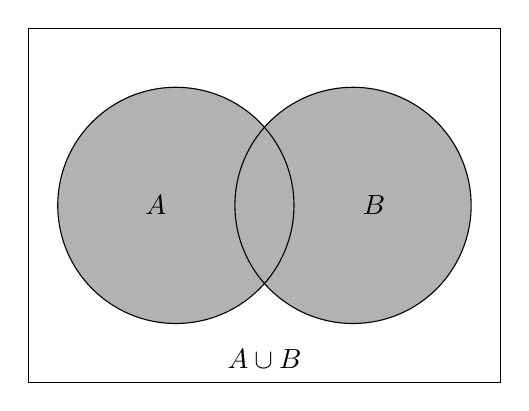
\begin{tikzpicture}[scale=1.5]
  
  \fill[gray!60] (-0.75,0) circle (1cm);
  \fill[gray!60] (0.75,0) circle (1cm);
  
  
  \draw (-2,-1.5) rectangle (2,1.5);
  \draw (-0.75,0) circle (1cm) node[left] {$A$};
  \draw (0.75,0) circle (1cm) node[right] {$B$};
  
  
  \node at (0,-1.3) {$A \cup B$};
\end{tikzpicture}
\end{center}
\vspace{1cm}

\begin{enumerate}

\item \textbf{Example 1:}

Let  
\[
A = \{1,2,3\}, \quad B = \{3,4,5\}.
\]  

Then the union of $A$ and $B$ is  
\[
A \cup B = \{1,2,3,4,5\}.
\]  

Notice that the element 3, which is in both sets, only appears once in the union.

\item \textbf{Example 2:}

Let  

\[
A = \{1,2,3,4,5\}, \quad 
B = \{3,4,5,6,7\}, \quad
C = \{5,6,7,8,9\}.
\]  

We ask for  

\[
U = A \cup B \cup C.
\]  

first,  

\[
A \cup B = \{1,2,3,4,5,6,7\}.
\]  

Second,  

\[
(A \cup B) \cup C = \{1,2,3,4,5,6,7,8,9\}.
\]  

Hence,  

\[
\boxed{U = A \cup B \cup C = \{1,2,3,4,5,6,7,8,9\}}
\]

\item \textbf{Example 3:}

Let  

\[
\begin{aligned}
A &= \left\{ x \in \mathbb{N}^+ \;\middle|\; \frac{x^2}{10} < 1 \right\} \\
B &= \left\{ x \in \mathbb{Z} \;\middle|\; -7 < x \leq -6 \right\}
\end{aligned}
\]

Since,

\[
A = \{1,2,3\}, \quad \text{and} \quad B = \{-6\}
\]

Therefore,
\[
\boxed{A \cup B = \{-6,1,2,3\}}
\]

\item \textbf{Example 4:}

Let $\mathcal{A}$ be a set whose elements are themselves sets. Then the union of all sets in $\mathcal{A}$, denoted $\displaystyle\bigcup \mathcal{A}$, is defined as:

\[
\displaystyle\bigcup \mathcal{A} = \{ x \mid \exists B \in \mathcal{A} \text{ such that } x \in B \}
\]

Examples:

\begin{enumerate}[label=\arabic*.]
    \item $\mathcal{A}_1 = \{ \{1,2\}, \{2,3\}, \{3,4\} \}$
    \[
    \displaystyle\bigcup \mathcal{A}_1 = \{1,2,3,4\}
    \]

    \item $\mathcal{A}_2 = \{ \{ \{1\}, \{2\} \}, \{ \{2\}, \{3\} \} \}$
    \[
    \displaystyle\bigcup \mathcal{A}_2 = \{ \{1\}, \{2\}, \{3\} \}
    \]

    \item $\mathcal{A}_3 = \{ \{a,b\}, \{b,c\}, \{c,d\}, \{d,a\} \}$
    \[
    \displaystyle\bigcup \mathcal{A}_3 = \{a,b,c,d\}
    \]
\end{enumerate}

\item \textbf{Example 5:}

Let  

\[
\begin{aligned}
A &= \left\{ x \in \mathbb{R} \;\middle|\; -8 - x > -\frac{x}{4} - 12 \right\} \\
B &= \left\{ x \in \mathbb{R} \;\middle|\; 30 - 2x < -\frac{x}{2} + 1 - 2x \right\}
\end{aligned}
\]

Since,

\[
A = \displaystyle\left(-\infty,\frac{16}{3}\right),
\quad
B = (-\infty,-58)
\]

Therefore,  

\[
\boxed{A \cup B = \left(-\infty,\frac{16}{3}\right)}
\]

\item \textbf{Example 6:}

Let  

\[
X = \{\alpha \mid \alpha \in \mathbb{Z}\}.
\]  

In this case, because the interval of $\mathbb{Z}$ is $(-\infty, \infty)$, we can systematically enumerate the set of integers by pairing each positive integer with its negative counterpart. Explicitly,

\[
X = \{..., -3, -2, -1, 0, 1, 2, 3, ...\}.
\]  

More formally, we can express this as  

\[
X = \{0\} \cup \displaystyle\bigcup_{n=1}^{\infty} \{-n, n\}.
\]  

This approach allows us to systematically enumerate all integers by pairing positive and negative integers together, ensuring we cover the entire infinite set $\mathbb{Z}$. Moreover, note that $\{0\}$ is a singleton set with exactly one element, and for each natural number $n \geq 1$, the set $\{-n, n\}$ has exactly two elements. In this way, $X$ is obtained by taking infinitely many of these finite pieces and joining them together using union operations, one for each $n \in \mathbb{N}$.  

Since the union runs over all natural numbers, we are forming what is called a countable union of finite sets. This construction demonstrates how union operations can systematically combine finite pieces to build infinite structures. Although this union process never ends, it grows step by step in correspondence with the natural numbers. We can think of this construction as building our set incrementally:

\[
X_0 = \{0\}
\]

\[
X_1 = X_0 \cup \{-1,1\}
\]

\[
X_2 = X_1 \cup \{-2,2\}
\]

\[
X_3 = X_2 \cup \{-3,3\}
\]

\[
\vdots
\]

So in general,

\[
X_n = \{0\} \cup \displaystyle\bigcup_{k=1}^n \{-k,k\}
\]

Therefore,

\[
X = \displaystyle\bigcup_{n=0}^\infty X_n = \mathbb{Z}.
\]

Because this construction systematically organizes every integer through union operations indexed by the natural numbers, we can see how infinite unions work in practice. Each step adds new elements while preserving all previous ones, and the union operation ensures that every integer appears exactly once in the final set. This example illustrates the power of union operations in constructing complex infinite sets from simple finite components.

\item \textbf{Example 7:}

Let  

\[
\mathbb{Z} \cup \mathbb{N}.
\]

Therefore, the union of $\mathbb{Z}$ and $\mathbb{N}$ is clearly $\mathbb{Z}$.

\emph{Proof.}

By using the Axiom of Union:

\[
\forall x \, \exists y \, \forall \alpha \,\big(\alpha \in y \;\leftrightarrow\; \exists z \, (z \in x \land \alpha \in z)\big).
\]

Intuitively, for any set $x$, there exists a set $y$ (its union) containing exactly those elements that belong to at least one member of $x$.

Now take $x = \{\mathbb{Z}, \mathbb{N}\}$. Then the axiom guarantees the existence of a set $y$ such that:

\[
\forall \alpha \;\;\big(\alpha \in y \;\leftrightarrow\; (\alpha \in \mathbb{Z} \lor \alpha \in \mathbb{N})\big).
\]

Thus $y = \mathbb{Z} \cup \mathbb{N}$.

But since $\mathbb{N} \subseteq \mathbb{Z}$, we have:

\[
\forall \alpha \;\; (\alpha \in \mathbb{N} \;\to\; \alpha \in \mathbb{Z}).
\]

Hence,

\[
\alpha \in \mathbb{Z} \cup \mathbb{N}
\;\;\leftrightarrow\;\;
(\alpha \in \mathbb{Z} \lor \alpha \in \mathbb{N})
\;\;\leftrightarrow\;\;
\alpha \in \mathbb{Z}.
\]

As a result,

\[
\boxed{\mathbb{Z} \cup \mathbb{N} = \mathbb{Z}.
\;\;\text {QED}
}
\]

\end{enumerate}

\section{Intersection}

The symbolic notation for intersection is:

\[
A \cap B = \{x \mid x \in A \land x \in B\}
\]

Moreover, if two sets have no common element, then the two sets are \emph{disjoint}. Formally:

\[
A \cap B = \varnothing
\]

\begin{center}
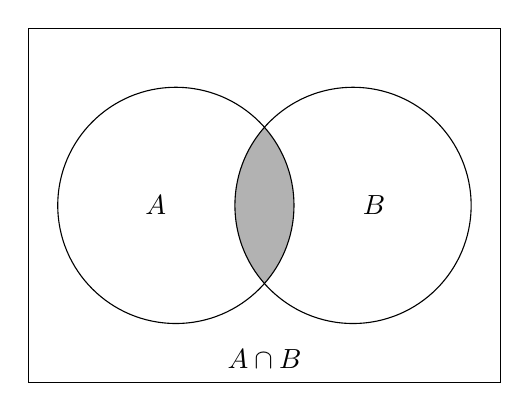
\begin{tikzpicture}[scale=1.5]
  
  \begin{scope}
    \clip (-0.75,0) circle (1cm);
    \fill[gray!60] (0.75,0) circle (1cm);
  \end{scope}
  
  \draw (-2,-1.5) rectangle (2,1.5);
  \draw (-0.75,0) circle (1cm) node[left] {$A$};
  \draw (0.75,0) circle (1cm) node[right] {$B$};
  
  
  \node at (0,-1.3) {$A \cap B$};
\end{tikzpicture}
\end{center}
\vspace{1cm}

\begin{enumerate}

\item \textbf{Example 1:}

Let
 
\[
P = \{a, b, c, d\}, \quad Q = \{b, d, e, f\}.
\]

The intersection of $P$ and $Q$ contains only the elements that are in both sets:

\[
\boxed{P \cap Q = \{b, d\}}
\]

Notice that $a$, $c$, $e$, and $f$ are excluded because they are not in both sets.

\item \textbf{Example 2:}

Consider three sets:

\[
M = \{1, 3, 5, 7\}, \quad
N = \{3, 4, 5, 6\}, \quad
O = \{0, 2, 5, 8\}.
\]

We want the elements that all three sets share:

Only the number $5$ appears in $M$, $N$, and $O$:

\[
M \cap N \cap O = \{5\}.
\]

Hence, the intersection is:

\[
\boxed{M \cap N \cap O = \{5\}}
\]

\item \textbf{Example 3:}

Let  

\[
\begin{aligned}
A &= \left\{ x \in \mathbb{Z} \;\middle|\; 0 \le x \le 10 \right\} \\
B &= \left\{ x \in \mathbb{Z} \;\middle|\; 7 \le x \le 12 \right\}
\end{aligned}
\]

Since the set $A$ is

\[
A = \{0, 1, 2, 3, 4, 5, 6, 7, 8, 9, 10\}
\]

and the set $B$ is

\[
B = \{7, 8, 9, 10, 11, 12\},
\]

we have

\[
\boxed{A \cap B = \{7, 8, 9, 10\}}
\]

\item \textbf{Example 4:}

Let  

\[
\begin{aligned}
C &= \left\{ x \in \mathbb{N}^+ \;\middle|\; |x - 5| < 4 \right\} \\
D &= \left\{ x \in \mathbb{Z} \;\middle|\; 3x - 7 = 2 \right\} \\
E &= \left\{ x \in \mathbb{N}^+ \;\middle|\; |2x - 10| \le 6 \right\} \\
F &= \left\{ x \in \mathbb{Z} \;\middle|\; |x + 1| = 7 \right\} \\
G &= \left\{ x \in \mathbb{N}^+ \;\middle|\; |x - 12| > 5 \right\}.
\end{aligned}
\]

Since,

\[
C = \{2,3,4,5,6,7,8\}
\]

\[
D = \{3\}
\]

\[
E = \{2,3,4,5,6,7,8\}
\]

\[
F = \{-8, 6\}
\]

For $G$, since $x \in \mathbb{N}^+$,  
\[
G = \{1,2,3,4,5,6\} \cup \{18,19,20,\dots\}
\]

Hence

\begin{enumerate}[label=\arabic*.]
    \item $C \cap D = \{3\}$  
    \item $C \cap E = \{2,3,4,5,6,7,8\}$ (same set)  
    \item $C \cap F = \{6\}$  
    \item $E \cap F = \{6\}$  
    \item $C \cap G = \{2,3,4,5,6\}$  
    \item $E \cap G = \{2,3,4,5,6\}$  
    \item $D \cap G = \{3\}$
\end{enumerate}

We conclude that,

\[
\boxed{C \cap D \cap E \cap F \cap G = \varnothing}
\]

\item \textbf{Example 5:}

Let  

\[
\begin{aligned}
A &= \left\{ x \in \mathbb{N}^+ \;\middle|\; \frac{3x - 4}{5} \le 7 \right\} \\
B &= \left\{ x \in \mathbb{Z} \;\middle|\; \frac{2x + 9}{4} = \frac{5x - 1}{6} \right\}
\end{aligned}
\]

Since the set $A$ is

\[
A = \{1, 2, 3, 4, 5, 6, 7, 8, 9, 10, 11, 12\}
\]

and the set $B$ is

\[
B = \varnothing \quad \text{(since $\displaystyle\frac{29}{4} \notin \mathbb{Z}$)},
\]

we have

\[
\boxed{A \cap B = \varnothing}
\]

\item \textbf{Example 6:}

Suppose

\[
A = \{ \{a,b\}, \{a,d,e\}, \{a,d\} \}
\]

In this case, we will answer by using intersection over the set. Therefore, the intersection over all subsets of $A$ is:

\[
\displaystyle\bigcap A = \bigcap_{X \in A} X
\]

The element common to all subsets is $a$, so:

\[\boxed{\displaystyle\bigcap A = \{a\}}\]

\item \textbf{Example 7:}

We can also define union and intersection over an indexed collection of sets $A_1, A_2, \dots$:

\[
\begin{aligned}
\bigcup_i A_i &= \{x \mid x \in A_i \text{ for some } i\} \\
\bigcap_i A_i &= \{x \mid x \in A_i \text{ for all } i\}
\end{aligned}
\]

If $I$ is an index set and we are considering $A_i$ for each $i \in I$, then:

\[
\begin{aligned}
\bigcup_{i \in I} A_i &= \{x \mid x \in A_i \text{ for some } i \in I\} \\
\bigcap_{i \in I} A_i &= \{x \mid x \in A_i \text{ for all } i \in I\}
\end{aligned}
\]

Let the index set be:

\[
I = \{1, 2, 3\}
\]

Define a family of sets $\{A_i\}_{i \in I}$ :

\[
\begin{aligned} A_1 &= \displaystyle \left\{ x \in \mathbb{Z} \;\middle|\; \frac{x-1}{x} = \frac{6}{3} \right\} \\ A_2 &= \displaystyle \left\{ y \in \mathbb{R} \;\middle|\; \frac{y+8}{12} = \frac{5y+6}{4} \right\} \\ A_3 &= \displaystyle \left\{ z \in \mathbb{N} \;\middle|\; -11(z+9) = -6 + 5\left[-z - \frac{99}{5}\right] \right\} \end{aligned}
\]

Then we compute:

\[
\displaystyle \bigcup_{i \in I} A_i = A_1 \cup A_2 \cup A_3, 
\quad
\displaystyle \bigcap_{i \in I} A_i = A_1 \cap A_2 \cap A_3
\]

Since the sets are

\[
A_1 = \{-1\}, \quad A_2 = \left\{-\displaystyle\frac{5}{7}\right\}, \quad A_3 = \{1\},
\]

Hence,

\[
\boxed{\displaystyle \bigcup_{i \in I} A_i = \left\{-1, -\frac{5}{7}, 1\right\}, \quad \displaystyle \bigcap_{i \in I} A_i = \varnothing}
\]

\item \textbf{Example 8:}

Example 1:

Let the index set be:

\[
I = \mathbb{N}
\]

Define a family of sets:

\[
A_i = \{ i, i+1, \dots, i^2 \}
\]

Therefore, the first few sets are:

\[
\begin{aligned}
A_1 &= \{1\}, \\
A_2 &= \{2, 3, 4\}, \\
A_3 &= \{3, 4, 5, 6, 7, 8, 9\}, \\
&\vdots
\end{aligned}
\]

Finally, the intersection remains:

\[
\displaystyle\bigcap_{i \in \mathbb{N}} A_i = \varnothing
\]

while the union of all sets in the family is:
\[
\displaystyle\bigcup_{i \in \mathbb{N}} A_i = \mathbb{N}
\]

Example 2:

Let the index set be:

\[
I = \mathbb{Z}
\]

Define a family of sets:

\[
A_i = (i-1, i)
\]

Therefore, the first few sets are:

\[
\begin{aligned}
A_{-2} &= (-3, -2), \\
A_{-1} &= (-2, -1), \\
A_0 &= (-1, 0), \\
A_1 &= (0, 1), \\
A_2 &= (1, 2), \\
A_3 &= (2, 3), \\
&\vdots
\end{aligned}
\]

Finally, the intersection of all sets is:

\[
\displaystyle\bigcap_{i \in \mathbb{Z}} A_i = \varnothing
\]

and the union of all sets is:

\[
\displaystyle\bigcup_{i \in \mathbb{Z}} A_i = \mathbb{R}.
\]

\end{enumerate}

\section{Difference}


The difference of sets $A$ and $B$, written $A \setminus B$ or $A - B$ is the set of all elements of $A$ that are not in $B$:

\[
A \setminus B = \{x \mid x \in A \land x \notin B\}
\]

\begin{center}
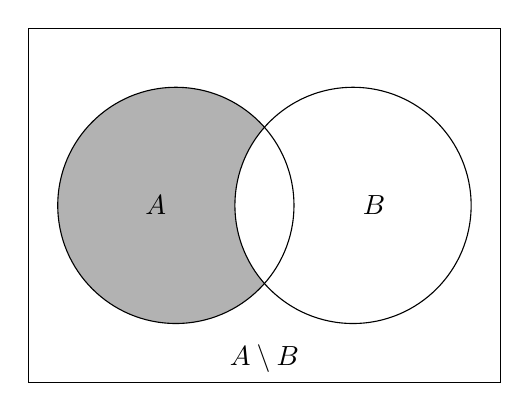
\begin{tikzpicture}[scale=1.5]
  
  \fill[gray!60] (-0.75,0) circle (1cm);
  
  \begin{scope}
    \clip (-0.75,0) circle (1cm);
    \fill[white] (0.75,0) circle (1cm);
  \end{scope}
  
  
  \draw (-2,-1.5) rectangle (2,1.5);
  \draw (-0.75,0) circle (1cm) node[left] {$A$};
  \draw (0.75,0) circle (1cm) node[right] {$B$};
  
  
  \node at (0,-1.3) {$A \setminus B$};
\end{tikzpicture}
\end{center}
\vspace{1cm}

\begin{enumerate}

\item \textbf{Example 1:}

Let

\[
A = \{apple, banana, cherry, date\}, \quad B = \{banana, date, fig\}.
\]

The difference $A - B$ consists of elements in $A$ that are not in $B$:

\[\boxed{A - B = \{apple, cherry\}}\]

Here, $banana$ and $date$ are removed because they are present in $B$.

\item \textbf{Example 2:}

Consider three sets:

\[
X = \{red, blue, green, yellow\}, \quad
Y = \{blue, yellow, purple\}, \quad
Z = \{yellow, orange\}.
\]

We want the elements in $X$ that are not in $Y$ or $Z$:

Remove elements of $Y$ from $X$ first:

\[
X - Y = \{red, green\}.
\]

Then remove elements of $Z$ (no change since $red$ and $green$ are not in $Z$):

\[
(X - Y) - Z = \{red, green\}.
\]

Hence, the difference is:

\[\boxed{X - Y - Z = \{red, green\}}\]

\item \textbf{Example 3:}

Let  

\[
\begin{aligned}
A &= \left\{ x \in \mathbb{Z} \;\middle|\; -1 \le x \le 6 \right\} \\
B &= \left\{ x \in \mathbb{Z} \;\middle|\; x \ge 2 \right\}
\end{aligned}
\]

Since the set $A$ is

\[
A = \{-1, 0, 1, 2, 3, 4, 5, 6\}
\]

and the set $B$ is

\[
B = \{2, 3, 4, 5, 6, 7, 8, \dots\},
\]

we have

\[\boxed{A \setminus B = \{-1, 0, 1\}}\]

\item \textbf{Example 4:}

Let  

\[
\mathbb{Z} = \displaystyle\bigcup_{k=-\infty}^{\infty} \{k\}, 
\quad 
\mathbb{N}^+ = \bigcup_{k=0}^{\infty} \{k+1\}.
\]

Then the difference is  

\[
\mathbb{Z} \setminus \mathbb{N}^+ = \{ z \in \mathbb{Z} \mid z \le 0 \}.
\]

So the result is the set of all non-positive integers:

\[\boxed{\displaystyle\bigcup_{k=-\infty}^{0} \{k\} = (-\infty, 0] \cap \mathbb{Z}}\]

\item \textbf{Example 5:}

Let the index set be:
\[I = \{1,2,3\}\]

Define the family of sets $\{A_i\}_{i \in I}$:

\[\begin{aligned}
A_1 &= \left\{ x \in \mathbb{N} \;\middle|\; \frac{3x-7}{4} = \frac{6x}{2} + \frac{49}{7} \right\} \\
A_2 &= \left\{ y \in \mathbb{Z} \;\middle|\; \frac{2y+9}{3} \le 6 \right\} \\
A_3 &= \left\{ z \in \mathbb{R} \;\middle|\; \frac{5z-11}{2} > 4 \right\}
\end{aligned}\]

Since:

\[A_1 = \varnothing, \quad 
A_2 = \{ x \in \mathbb{Z} \mid x \le 4 \}, \quad 
A_3 = \{ x \in \mathbb{R} \mid x > \displaystyle\frac{19}{5} \}\]

Therefore:

\[\displaystyle\bigcup_{i \in I} A_i = \{ x \in \mathbb{R} \mid x > \frac{19}{5} \} \cup \{ x \in \mathbb{Z} \mid x \le 4 \}, \quad
\bigcap_{i \in I} A_i = \varnothing\]

We conclude:

\[\boxed{\left( \displaystyle\bigcup_{i \in I} A_i \right) \setminus \left( \bigcap_{i \in I} A_i \right) = \{ x \in \mathbb{R} \mid x > \frac{19}{5} \} \cup \{ x \in \mathbb{Z} \mid x \le 4 \}}\]

\item \textbf{Example 6:}

Let

\[
\begin{aligned}
A &= \left\{ x \in \mathbb{R} \;\middle|\; \frac{x}{2} + \frac{1}{3} < \frac{2x}{5} \right\} \\
B &= \left\{ y \in \mathbb{N} \;\middle|\; 2 < \frac{y-1}{3} \le 6 \right\} \\
C &= \left\{ z \in \mathbb{Z} \;\middle|\; -5 \leq z \leq 10 \right\}
\end{aligned}
\]

Since

\[
\begin{aligned}
A = \left(-\infty, -\frac{10}{3}\right), \quad
B = (7, 19] \cap \mathbb{N}, \quad 
C = [-5, 10] \cap \mathbb{Z}
\end{aligned}
\]

Thus, 
\[
A \cap B = \varnothing
\]

We conclude that,

\[\boxed{(A \cap B) \setminus C = \varnothing}\]

\end{enumerate}

\section{Symmetric Difference}

The symmetric difference of sets $A$ and $B$, written $A \triangle B$, is the set of all elements that are in either $A$ or $B$ but not in both:

\[
A \triangle B =  (A \cup B) \setminus (A \cap B).
\]

\begin{center}
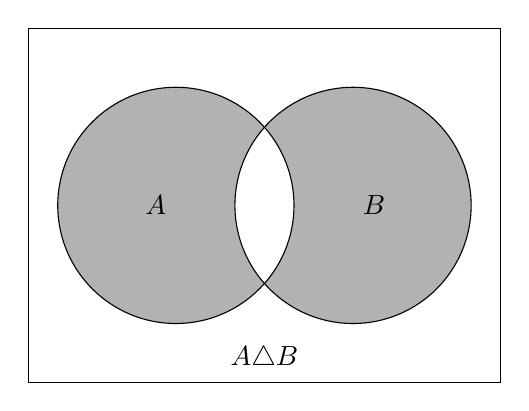
\begin{tikzpicture}[scale=1.5]
  
  \fill[gray!60] (-0.75,0) circle (1cm);
  \fill[gray!60] (0.75,0) circle (1cm);
  
  \begin{scope}
    \clip (-0.75,0) circle (1cm);
    \fill[white] (0.75,0) circle (1cm);
  \end{scope}
  
  
  \draw (-2,-1.5) rectangle (2,1.5);
  \draw (-0.75,0) circle (1cm) node[left] {$A$};
  \draw (0.75,0) circle (1cm) node[right] {$B$};
  
  
  \node at (0,-1.3) {$A \triangle B$};
\end{tikzpicture}
\end{center}
\vspace{1cm}

\begin{enumerate}

\item \textbf{Example 1:}

Let  
\[
A = \{1, 2, 3, 4\}, \quad B = \{3, 4, 5, 6\}.
\]

The symmetric difference consists of elements that belong to exactly one of the two sets. Hence,
\[
\boxed{A \,\Delta\, B = \{1, 2, 5, 6\}}
\]

The elements $3$ and $4$ are excluded since they appear in both $A$ and $B$.

\item \textbf{Example 2:}

Consider three sets:
\[
X = \{1, 2, 3, 4\}, \quad
Y = \{3, 4, 5, 6\}, \quad
Z = \{4, 5, 6, 7\}.
\]

First, compute the symmetric difference of $X$ and $Y$:
\[
X \,\Delta\, Y = \{1, 2, 5, 6\}.
\]

Next, compute the symmetric difference with $Z$:
\[
\{1, 2, 5, 6\} \,\Delta\, \{4, 5, 6, 7\} = \{1, 2, 4, 7\}.
\]

Therefore,
\[
\boxed{X \,\Delta\, Y \,\Delta\, Z = \{1, 2, 4, 7\}}
\]

\item \textbf{Example 3:}

Let
\[
\begin{aligned}
A &= \left\{ (p,q) \in \mathbb{N}^2 \;\middle|\; \frac{3p+2q}{p} \ge 9,\; p \neq 0 \right\}, \\
B &= \left\{ x \in \mathbb{Z}^+ \;\middle|\; \frac{x-1}{x} = x+1 \right\}.
\end{aligned}
\]

Since
\[
A = \bigcup_{p=1}^{\infty} \{p\} \times \big([3p,\infty) \cap \mathbb{N}\big),
\]
and
\[
B = \varnothing,
\]
we have
\[
A \cap B = \varnothing.
\]

Since the sets are disjoint,
\[
A \triangle B = A.
\]

Thus,
\[
\boxed{
A \triangle B
= \bigcup_{p=1}^{\infty} \{p\} \times \big([3p,\infty) \cap \mathbb{N}\big)
}
\]

\item \textbf{Example 4:}

Let
\[
\begin{aligned}
A &= \{p \in \mathbb{R} \mid -4(p-4) \ge -2(p+1)\}, \\
B &= \{q \in \mathbb{R} \mid -46 < 4q - 6 \le -26\}, \\
C &= \{r \in \mathbb{R} \mid -(1 + 2r) > -6(r-4) - 1\}.
\end{aligned}
\]

Solving the inequalities gives
\[
A = (-\infty, 9], \quad
B = (-10, -5], \quad
C = (6, \infty).
\]

Hence,
\[
A \cup B = (-\infty, 9], \quad
C \setminus A = (9, \infty).
\]

Since these sets are disjoint,
\[
(A \cup B) \triangle (C \setminus A)
= (-\infty, 9] \cup (9, \infty)
= (-\infty, \infty).
\]

Therefore,
\[
\boxed{(A \cup B) \triangle (C \setminus A) = (-\infty, \infty)}
\]

\item \textbf{Example 5:}

Let
\[
A = \bigcup_{n\in\mathbb{N}} \{f^k(n) : k \ge 0\}, \quad
B = \bigcup_{k\in\mathbb{N}} \{k^2 - k + 1\},
\]
where
\[
f(n) =
\begin{cases}
\dfrac{n}{2}, & \text{if $n$ is even},\\[2mm]
3n + 1, & \text{if $n$ is odd}.
\end{cases}
\]

Since $f^0(n) = n$, every natural number belongs to $A$, hence
\[
A = \mathbb{N}.
\]

Therefore,
\[
A \cup B = \mathbb{N}, \quad A \cap B = B.
\]

We conclude that,
\[
\boxed{
A \triangle B
= \{\, m \in \mathbb{N} \mid m \neq k^2 - k + 1
\text{ for any } k \in \mathbb{N} \,\}
}
\]

\end{enumerate}

\section{Complement}

The symbolic notation for Complement is:  

\[
A^c = \{\, x \in U \mid x \notin A \,\}
\]

\begin{center}
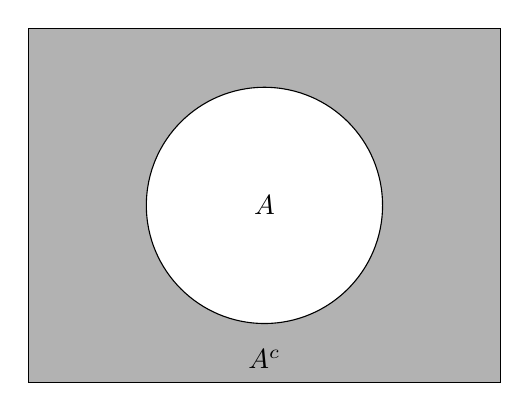
\begin{tikzpicture}[scale=1.5]
  
  \fill[gray!60] (-2,-1.5) rectangle (2,1.5);
  
  \fill[white] (0,0) circle (1cm);
  
  \draw (-2,-1.5) rectangle (2,1.5);
  \draw (0,0) circle (1cm) node {$A$};
  
  
  \node at (0,-1.3) {$A^c$};
\end{tikzpicture}
\end{center}
\vspace{1cm}

\begin{enumerate}

\item \textbf{Example 1:}

Let  
\[
U = \{1, 2, 3, 4, 5, 6\} \quad \text{(the universal set)}, 
\quad A = \{2, 4, 6\}.
\]

Hence,
\[
\boxed{A^c = \{1, 3, 5\}}
\]

The elements $2$, $4$, and $6$ are excluded since they belong to $A$.

\item \textbf{Example 2:}

Consider the universal set and two subsets:
\[
U = \{1, 2, 3, 4, 5, 6, 7, 8, 9\}, \quad
B = \{1, 3, 5, 7, 9\}, \quad
C = \{2, 3, 4, 5\}.
\]

The complement of $B$ in $U$ is
\[
\boxed{B^c = \{2, 4, 6, 8\}}.
\]

The complement of $C$ in $U$ is
\[
\boxed{C^c = \{1, 6, 7, 8, 9\}}.
\]

\item \textbf{Example 3:}

Let
\[
A = \bigcup_{k \in \mathbb{N}} \{\,2k+1\,\}, \quad
B = \bigcup_{k \in \mathbb{N}} \{\,2k\,\}.
\]

Since $A$ is the set of odd natural numbers and $B$ is the set of even natural numbers, we have
\[
\boxed{B^c = \mathbb{N} \setminus B = A}.
\]

\item \textbf{Example 4:}

Let
\[
A = \{\, p \in \mathbb{P} \mid p+2 \in \mathbb{P} \,\},
\]
that is, $A$ is the set of primes $p$ such that $p+2$ is also prime.

Let
\[
U = \bigcup_{k \in \mathbb{N}} \{\,2k+1\,\}
= \{1, 3, 5, 7, 9, 11, 13, \dots\}.
\]

Then the complement of $A$ relative to $U$ is
\[
A^c = U \setminus A.
\]

Hence,
\[
\boxed{
A^c
= \{\,2k+1 \mid k \in \mathbb{N}\,\}
\setminus
\{\, p \in \mathbb{P} \mid p+2 \in \mathbb{P} \,\}
}
\]

\item \textbf{Example 5:}

Let
\[
L = \{\, (x, y) \in \mathbb{R}^2 \mid y - 3 = x - 2 \,\}.
\]

Thus, $L$ is the line of slope $1$ passing through the point $(2,3)$.

Let
\[
A = \{\, (x, y) \in \mathbb{R}^2 \mid y > x + 1 \,\},
\]
the set of points strictly above the line $y = x + 1$.

The complement of $A$ relative to $\mathbb{R}^2$ is
\[
A^c = \mathbb{R}^2 \setminus A.
\]

That is,
\[
\boxed{
A^c
= \bigcup_{x \in \mathbb{R}}
\{\, (x, y) \in \mathbb{R}^2 \mid y \le x + 1 \,\}
= B \cup L
}
\]

where
\[
B = \{\, (x, y) \in \mathbb{R}^2 \mid y < x + 1 \,\},
\quad
L = \{\, (x, y) \in \mathbb{R}^2 \mid y = x + 1 \,\}.
\]

\end{enumerate}


\begin{center}
\resizebox{0.55\textwidth}{!}{
\begin{tikzpicture}
    
    \draw[thick, fill=white] (-8,-8) rectangle (8,8);

    \draw[thick,->] (-6,0) -- (6.5,0) node[anchor=north west] {$x$};
    \draw[thick,->] (0,-6) -- (0,6.5) node[anchor=south east] {$y$};
    \node[anchor=north east] at (0,0) {$0$};

    \foreach \x in {-5,-4,-3,-2,-1,1,2,3,4,5}
        \draw (\x,1pt) -- (\x,-1pt) node[anchor=north] {$\x$};

    \foreach \y in {-5,-4,-3,-2,-1,1,2,3,4,5}
        \draw (1pt,\y) -- (-1pt,\y) node[anchor=east] {$\y$};

    \draw[thick, gray!60!black] (-5,-4) -- (5,6);

    \fill[red!60!black] (2,3) circle (2pt);
    \node[right=2mm] at (2,3) {$(2,3)$};

    \fill[red!60!black] (0,1) circle (2pt);
    \node[left=2mm] at (0,1) {$(0,1)$};

    \node[gray!80!black] at (-3,5) {$A = y > x + 1$};
    \node[gray!80!black] at (2,-5) {$A^c = B \cup L$};

\end{tikzpicture}
}
\end{center}

\section{Cartesian Product}

It follows from the Axiom of Extensionality that sets have no intrinsic order to their elements. For instance, in an unordered pair  

\[
\{x, y\} = \{y, x\}
\]

the order does not matter.  

However, when we need to represent ordered structures, we use ordered pairs, written $\langle x, y \rangle$. Here, order does matter:  

\[
\langle x, y \rangle \neq \langle y, x \rangle \quad \text{if } x \neq y
\]

An ordered pair $\langle a, b \rangle$ is defined in set theory using the \emph{Wiener--Kuratowski} definition:  

\[
\langle a, b \rangle := \{\{a\}, \{a, b\}\}
\]

This definition guarantees that  

\[
\langle a, b \rangle = \langle c, d \rangle \leftrightarrow a = c \ \text{and}\ b = d
\]

\emph{Proof.}

Suppose  

\[
\langle a, b \rangle = \langle c, d \rangle.
\]

By definition, this means  

\[
\{\{a\}, \{a, b\}\} = \{\{c\}, \{c, d\}\}.
\]

So the two sets have the same elements. There are two cases:

\begin{enumerate}
\item If $\{a\} = \{c\}$, then $a = c$.  
Then $\{a, b\} = \{c, d\}$, so $\{a, b\} = \{a, d\}$.  
This forces $b = d$.

\item If $\{a\} = \{c, d\}$, then $\{a\}$ must have two elements unless $c = d$.  
But $\{a\}$ has only one element, so $c = d$ and $a = c = d$.  
Then from $\{a, b\} = \{c\} = \{a\}$, we get $b = a = d$.
\end{enumerate}

Thus in either case, $a = c$ and $b = d$.

If $a = c$ and $b = d$, then clearly  

\[
\langle a, b \rangle
= \{\{a\}, \{a, b\}\}
= \{\{c\}, \{c, d\}\}
= \langle c, d \rangle.
\]

Hence,  

\[
\langle a, b \rangle = \langle c, d \rangle
\leftrightarrow a = c \ \text{and}\ b = d. \quad Q.E.D.
\]

The idea of ordered pairs can be extended to longer sequences. For example, a triple

$\langle x, y, z \rangle$ is represented as $\langle \langle x, y \rangle, z \rangle$, and a quadruple
$\langle x, y, z, u \rangle$ is $\langle \langle \langle x, y \rangle, z \rangle, u \rangle$.

In general, an ordered $n$-tuple is defined as nested ordered pairs:

\[
\langle x_1, x_2, \ldots, x_n \rangle
\]

With this in mind, we can now define the Cartesian product. Since order matters, we collect all possible ordered pairs with the first element taken from $A$ and the second from $B$:

\[
A \times B = \{ \langle a, b \rangle \mid a \in A \wedge b \in B \}
\]

For example, let  

\[
\begin{aligned}
A &= \{0, 1\} \\
B &= \{1, a, b\}
\end{aligned}
\]

Then the Cartesian product is  

\[
\begin{array}{|c|c|c|}
\hline
\langle 0,1 \rangle & \langle 0,a \rangle & \langle 0,b \rangle \\ \hline
\langle 1,1 \rangle & \langle 1,a \rangle & \langle 1,b \rangle \\ \hline
\end{array}
\]

\begin{center}
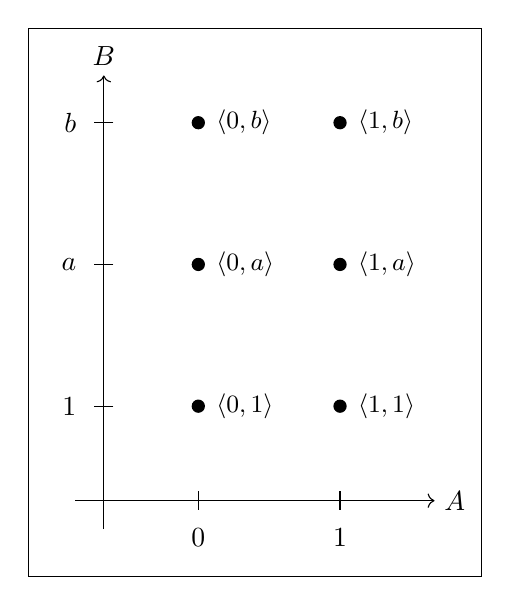
\begin{tikzpicture}[scale=1.2]
    
    \draw (-0.8,-0.8) rectangle (4,5);
    
    
    \draw[->] (-0.3,0) -- (3.5,0) node[right] {$A$};
    \draw[->] (0,-0.3) -- (0,4.5) node[above] {$B$};

    
    \foreach \x/\label in {1/0, 2.5/1} {
        \draw (\x,0.1) -- (\x,-0.1) node[below=3pt] {$\label$};
    }

    
    \foreach \y/\label in {1/1, 2.5/a, 4/b} {
        \draw (0.1,\y) -- (-0.1,\y) node[left=3pt] {$\label$};
    }

    
    \foreach \x in {1,2.5} {
        \foreach \y in {1,2.5,4} {
            \fill[black] (\x,\y) circle (2pt);
        }
    }

    
    \node[anchor=west, xshift=3pt] at (1,1) {\small$\langle 0,1 \rangle$};
    \node[anchor=west, xshift=3pt] at (1,2.5) {\small$\langle 0,a \rangle$};
    \node[anchor=west, xshift=3pt] at (1,4) {\small$\langle 0,b \rangle$};

    \node[anchor=west, xshift=3pt] at (2.5,1) {\small$\langle 1,1 \rangle$};
    \node[anchor=west, xshift=3pt] at (2.5,2.5) {\small$\langle 1,a \rangle$};
    \node[anchor=west, xshift=3pt] at (2.5,4) {\small$\langle 1,b \rangle$};
\end{tikzpicture}
\end{center}

As we have seen, the cardinality $|A| = 2$ and $|B| = 3$. Hence,
\[
|A \times B| = 6.
\]

Note that the Cartesian product is not commutative:
\[
A \times B \neq B \times A.
\]

Indeed,
\[
A \times B =
\{\langle 0,1 \rangle, \langle 0,a \rangle, \langle 0,b \rangle,
  \langle 1,1 \rangle, \langle 1,a \rangle, \langle 1,b \rangle\},
\]
whereas
\[
B \times A =
\{\langle 1,0 \rangle, \langle 1,1 \rangle,
  \langle a,0 \rangle, \langle a,1 \rangle,
  \langle b,0 \rangle, \langle b,1 \rangle\}.
\]

Both sets have six elements, but they are different because order matters.
The Cartesian product can be extended to products of a set with itself. For a set $A$,

\[
\begin{aligned}
A^1 &= A, \\
A^2 &= A \times A, \\
A^3 &= A^2 \times A, \\
&\vdots \\
A^{k+1} &= A^k \times A.
\end{aligned}
\]

If $|A| = n$, then $|A^k| = n^k$ for all $k \ge 1$, as shown by induction. More generally, if $|A| = n$ and $|B| = m$, then

\[
|A \times B| = n \cdot m.
\]

Let

\[
C_x = \{\langle x,y \rangle \mid y \in B\}, \qquad x \in A.
\]

Each set $C_x$ has $m$ elements, the family $\{C_x\}_{x\in A}$ is pairwise disjoint, and

\[
A \times B = \bigcup_{x \in A} C_x.
\]

Cartesian powers naturally lead to the notion of words. A word of length $n$ over $A$ is an element of $A^n$. The set of all finite words over $A$ is the \emph{Kleene star}:

\[
A^* = \bigcup_{k=0}^{\infty} A^k,
\]

where $A^0 = \{\varnothing\}$ is the empty word.

\bigskip

\begin{enumerate}
\item \textbf{Example 1.}

Let
\[
A = \{1,2\}, \quad B = \{3,4\}.
\]

Then
\[
\begin{array}{|c|c|}
\hline
\langle 1,3 \rangle & \langle 1,4 \rangle \\ \hline
\langle 2,3 \rangle & \langle 2,4 \rangle \\ \hline
\end{array}
\]

Note that $\langle 1,3 \rangle \neq \langle 3,1 \rangle$.

\item \textbf{Example 2.}

Let
\[
X = \{1,2\}, \quad
Y = \{a,b\}, \quad
Z = \{0,9\}.
\]

First,
\[
X \times Y =
\{\langle 1,a \rangle, \langle 1,b \rangle,
  \langle 2,a \rangle, \langle 2,b \rangle\}.
\]

Then
\[
\begin{array}{|c|c|}
\hline
\langle \langle 1,a \rangle, 0 \rangle &
\langle \langle 1,a \rangle, 9 \rangle \\ \hline
\langle \langle 1,b \rangle, 0 \rangle &
\langle \langle 1,b \rangle, 9 \rangle \\ \hline
\langle \langle 2,a \rangle, 0 \rangle &
\langle \langle 2,a \rangle, 9 \rangle \\ \hline
\langle \langle 2,b \rangle, 0 \rangle &
\langle \langle 2,b \rangle, 9 \rangle \\ \hline
\end{array}
\]

\item \textbf{Example 3.}

Let
\[
A = \{1,2\}, \quad
B = \{3,4\}, \quad
C = \{5,6\}, \quad
D = \{7,8\}.
\]

The Cartesian product $A \times B \times C \times D$ consists of ordered quadruples:
\[
\begin{array}{|c|c|c|c|}
\hline
\langle \langle \langle 1,3 \rangle, 5 \rangle, 7 \rangle &
\langle \langle \langle 1,3 \rangle, 5 \rangle, 8 \rangle &
\langle \langle \langle 1,3 \rangle, 6 \rangle, 7 \rangle &
\langle \langle \langle 1,3 \rangle, 6 \rangle, 8 \rangle \\ \hline
\langle \langle \langle 1,4 \rangle, 5 \rangle, 7 \rangle &
\langle \langle \langle 1,4 \rangle, 5 \rangle, 8 \rangle &
\langle \langle \langle 1,4 \rangle, 6 \rangle, 7 \rangle &
\langle \langle \langle 1,4 \rangle, 6 \rangle, 8 \rangle \\ \hline
\langle \langle \langle 2,3 \rangle, 5 \rangle, 7 \rangle &
\langle \langle \langle 2,3 \rangle, 5 \rangle, 8 \rangle &
\langle \langle \langle 2,3 \rangle, 6 \rangle, 7 \rangle &
\langle \langle \langle 2,3 \rangle, 6 \rangle, 8 \rangle \\ \hline
\langle \langle \langle 2,4 \rangle, 5 \rangle, 7 \rangle &
\langle \langle \langle 2,4 \rangle, 5 \rangle, 8 \rangle &
\langle \langle \langle 2,4 \rangle, 6 \rangle, 7 \rangle &
\langle \langle \langle 2,4 \rangle, 6 \rangle, 8 \rangle \\ \hline
\end{array}
\]

\item \textbf{Example 4.}

\[
\begin{aligned}
A &= \{(x,y) \in \mathbb{R}^2 \mid y = \tfrac{3}{2}x - 1\}, \\
B &= \{(m,n) \in \mathbb{Z}^2 \mid m \ge 6n,\; m \neq 0\}.
\end{aligned}
\]

Thus,
\[
A \times B =
\left\{ \bigl((x,\tfrac{3}{2}x - 1),(m,n)\bigr)
\;\middle|\;
x \in \mathbb{R},\; m,n \in \mathbb{Z},\; m \ge 6n,\; m \neq 0
\right\}.
\]

\item \textbf{Example 5.}

Let
\[
A = \{\langle x \rangle \mid x \in \{p,q,r\}\}, \quad
B = \{\langle y \rangle \mid y \in \{0,1,2\}\}.
\]

Then

\[
\begin{array}{c@{\hskip 1.5cm}c}
\begin{aligned}
C_{\langle p \rangle} &= \{\langle p,0\rangle, \langle p,1\rangle, \langle p,2\rangle\} \\
C_{\langle q \rangle} &= \{\langle q,0\rangle, \langle q,1\rangle, \langle q,2\rangle\} \\
C_{\langle r \rangle} &= \{\langle r,0\rangle, \langle r,1\rangle, \langle r,2\rangle\}
\end{aligned}
&
\begin{array}{c|c|c|c}
 & 0 & 1 & 2 \\ \hline
p & \langle p,0\rangle & \langle p,1\rangle & \langle p,2\rangle \\
q & \langle q,0\rangle & \langle q,1\rangle & \langle q,2\rangle \\
r & \langle r,0\rangle & \langle r,1\rangle & \langle r,2\rangle
\end{array}
\end{array}
\]

\item \textbf{Example 6.}

Let

\[
I = [0,1], \qquad
A_\alpha = [\alpha,2] \times [0,\alpha].
\]

For selected values of $\alpha$:

\[
\begin{aligned}
A_0 &= [0,2] \times \{0\}, \\
A_{0.25} &= [0.25,2] \times [0,0.25], \\
A_{0.5} &= [0.5,2] \times [0,0.5], \\
A_{0.75} &= [0.75,2] \times [0,0.75], \\
A_1 &= [1,2] \times [0,1].
\end{aligned}
\]
\end{enumerate}

\begin{center}
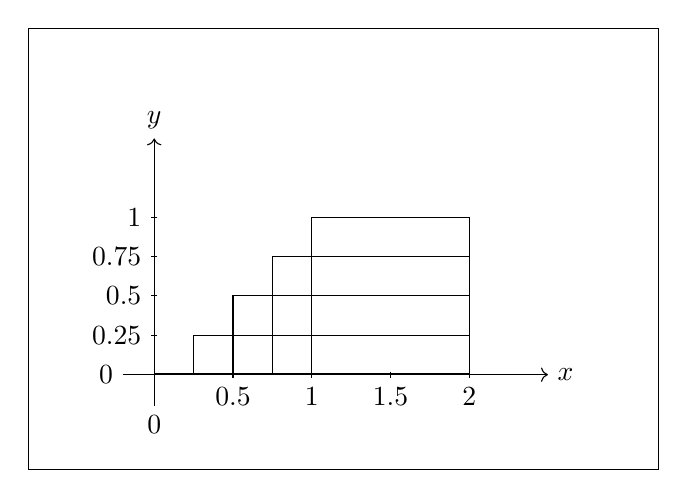
\begin{tikzpicture}[scale=2]
    
    \draw (-0.8,-0.6) rectangle (3.2,2.2);
    
    \draw[->] (-0.2,0) -- (2.5,0) node[right] {$x$};
    \draw[->] (0,-0.2) -- (0,1.5) node[above] {$y$};
    
    \draw (0,0) rectangle (2,0.01);      
    \draw (0.25,0) rectangle (2,0.25);   
    \draw (0.5,0) rectangle (2,0.5);     
    \draw (0.75,0) rectangle (2,0.75);   
    \draw (1,0) rectangle (2,1);         

    \foreach \x in {0.5,1,1.5,2} { 
        \draw (\x,0.02) -- (\x,-0.02) node[below] {\x};
    }
    \foreach \y in {0.25,0.5,0.75,1} {
        \draw (0.02,\y) -- (-0.02,\y) node[left] {\y};
    }
    
    
    \draw (0,0.02) -- (0,-0.02) node[below] at (0,-0.2) {$0$};  
    \draw (0.02,0) -- (-0.02,0) node[left] at (-0.2,0) {$0$};   

\end{tikzpicture}
\end{center}

\section{Subset}

The symbolic notation for subset is:

\[
A \subseteq B \leftrightarrow \forall x \, (x \in A \to x \in B)
\]

\begin{center}
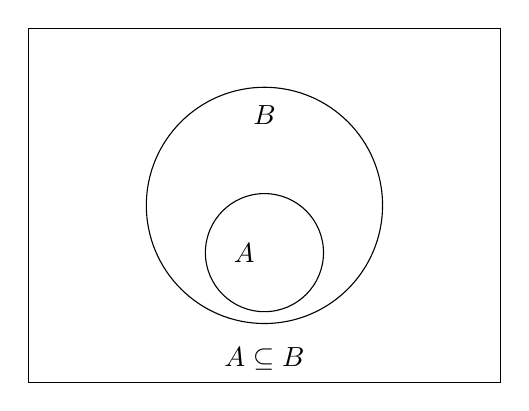
\begin{tikzpicture}[scale=1.5]
  
  \draw (-2,-1.5) rectangle (2,1.5);
  
  
  \draw (0,0) circle (1cm) node[above, yshift=0.9cm] {$B$};
  
  
  \draw (0,-0.4) circle (0.5cm) node[left] {$A$};
  
  
  \node at (0,-1.3) {$A \subseteq B$};
\end{tikzpicture}
\end{center}
\vspace{1cm}

If $A$ is not a subset of $B$, we write $A \nsubseteq B$. This means that there exists at least one element in $A$ that is not in $B$:

\[
A \nsubseteq B \leftrightarrow \exists x \, (x \in A \land x \notin B)
\]

Furthermroe, It's crucial to distinguish between an element of a set and a subset of a set:

\begin{enumerate}
\item $2 \in \mathbb{Z}$
\item $\mathbb{E} \subseteq \mathbb{Z}$ (the set of even numbers is a subset of the integers)  
\item A set can be both an element and a subset of another set. 
\end {enumerate}

For example:  

\[
\{1\} \in \{1, \{1\}\} \quad \text{and} \quad \{1\} \subseteq \{1, \{1\}\}
\]

This shows that a set can be both an element and a subset of another set:
\begin{enumerate}
\item $\{1\} \in \{1, \{1\}\}$, which means that the set $\{1\}$ appears as an element of the larger set.
\item $\{1\} \subseteq \{1, \{1\}\}$, since every element of $\{1\}$ (namely $1$) is also an element of the larger set.
\end{enumerate}

In contrast, the number $1$ itself is only an element and not a subset:
\begin{enumerate}
\item $1 \in \{1, \{1\}\}$, because $1$ is an element of the set.

\item $1 \nsubseteq \{1, \{1\}\}$, since $1$ is not a set and therefore cannot be a subset.
\end{enumerate}

\begin{enumerate}

\item \textbf{Example 1}

\[
A \subseteq B \;\;\to\;\; A \cup B = B
\]

\emph{Proof.}

By definition of subset,

\[
A \subseteq B \;\;\leftrightarrow\;\; \forall x \, (x \in A \to x \in B).
\]

By definition of union,

\[
A \cup B = \{x \mid x \in A \lor x \in B\}.
\]

Thus,

\[
x \in A \cup B 
\leftrightarrow
(x \in A \lor x \in B).
\]

Since $A \subseteq B$, we have $x \in A \to x \in B$, and therefore

\[
(x \in A \lor x \in B)
\leftrightarrow
(x \in B \lor x \in B)
\leftrightarrow
x \in B.
\]

Hence,

\[
\boxed{A \cup B = B. \quad \text{QED}}
\]

\item \textbf{Example 2}

\[
A \subseteq B \;\;\to\;\; A \cap B = A
\]

\emph{Proof.}

By definition of intersection,

\[
A \cap B = \{x \mid x \in A \land x \in B\}.
\]

Thus,

\[
x \in A \cap B 
\leftrightarrow
(x \in A \land x \in B).
\]

Since $A \subseteq B$, $x \in A$ implies $x \in B$, so

\[
(x \in A \land x \in B) \leftrightarrow x \in A.
\]

Therefore,

\[
\boxed{A \cap B = A. \quad \text{QED}}
\]

\item \textbf{Example 3}

Let

\[
A \in B.
\]

Then,

\[
A \subseteq \bigcup B.
\]

\emph{Proof.}

By definition,

\[
\bigcup B = \{x \mid \exists C \in B \; (x \in C)\}.
\]

If $x \in A$ and $A \in B$, then taking $C = A$ gives $x \in \bigcup B$. Hence,

\[
\boxed{A \subseteq \bigcup B. \quad \text{QED}}
\]

\item \textbf{Example 4}

Let

\[
A = \{1,2,3,4,5\}, \quad B = \{2,4\}.
\]

Every element of $B$ is an element of $A$, so

\[
\boxed{B \subseteq A}.
\]

\item \textbf{Example 5}

Let

\[
X = \{10,20,30,40\}, \quad
Y = \{10,20,30,40\}, \quad
Z = \{20,30\}.
\]

Then,

\[
\boxed{Y \subseteq X \quad \text{and} \quad Z \subseteq X}.
\]

\item \textbf{Example 6}

Let

\[
A = \{1,2,3\}, \quad B = \{3,2,1\}.
\]

By extensionality,

\[
A = B \leftrightarrow A \subseteq B \text{ and } B \subseteq A.
\]

Moreover, every set satisfies

\[
A \subseteq A,
\]

and for every set $A$,

\[
\boxed{\varnothing \subseteq A}.
\]

\item \textbf{Example 7}

\[
\mathbb{N}^+ \subseteq \mathbb{Z} \subseteq \mathbb{Q} \subseteq \mathbb{R}.
\]

Each inclusion is proper:

\[
\boxed{\mathbb{N}^+ \subsetneq \mathbb{Z} \subsetneq \mathbb{Q} \subsetneq \mathbb{R}}.
\]

Let

\[
\mathbb{B} = \{0,1\}.
\]

Then the Kleene star is

\[
\mathbb{B}^* = \{\Lambda, 0, 1, 00, 01, 10, 11, 000, \dots\}.
\]

For any string $x \in A^*$ with

\[
x = x_1 x_2 \dots x_n,
\]

its length is defined by

\[
\boxed{\operatorname{len}(x) = n}.
\]

\end{enumerate}

\section{Power Set}

The symbolic notation for the power set of a set $A$ is:

\[
\mathcal{P}(A) = \{x \mid x \subseteq A\}
\]

\begin {enumerate}

\item \textbf{Example 1.}

Let
\[
S = \{a,b\}.
\]

Then the power set of $S$ is

\[
\mathcal{P}(S) = \{\varnothing,\{a\},\{b\},\{a,b\}\}.
\]

Since $|S| = 2$, we have

\[
\boxed{|\mathcal{P}(S)| = 2^{|S|} = 2^2}.
\]

\bigskip

\item \textbf{Example 2.}

Let

\[
Y = \varnothing.
\]

Then

\[
\mathcal{P}(Y) = \{\varnothing\}.
\]

Hence,

\[
|\mathcal{P}(Y)| = 2^{|Y|} = 2^0 = 1.
\]

\bigskip

\item \textbf{Example 3.}

Let

\[
A = \{1,2,3\}.
\]

Then

\[
\mathcal{P}(A)
=
\{\varnothing,\{1\},\{2\},\{3\},\{1,2\},\{1,3\},\{2,3\},\{1,2,3\}\}.
\]

Thus,

\[
|\mathcal{P}(A)| = 2^{|A|} = 2^3.
\]

Let

\[
B = \mathcal{P}(\mathcal{P}(A)).
\]

Therefore,

\[
\boxed{|\mathcal{P}(\mathcal{P}(A))| = 2^{|\mathcal{P}(A)|} = 256}.
\]

\bigskip

\item \textbf{Example 4.}

Let

\[
A = \{1,2\}, \quad B = \{3,4\}.
\]

Define

\[
C = \mathcal{P}(A) \times \mathcal{P}(B).
\]

Since

\[
|\mathcal{P}(A)| = 2^{|A|}, \qquad
|\mathcal{P}(B)| = 2^{|B|},
\]

it follows that

\[
\boxed{|C| = 2^{|A|+|B|} = 16}.
\]

Explicitly,

\[
\begin{array}{|c|c|c|c|}
\hline
(\varnothing,\varnothing) & (\varnothing,\{3\}) & (\varnothing,\{4\}) & (\varnothing,\{3,4\}) \\ \hline
(\{1\},\varnothing) & (\{1\},\{3\}) & (\{1\},\{4\}) & (\{1\},\{3,4\}) \\ \hline
(\{2\},\varnothing) & (\{2\},\{3\}) & (\{2\},\{4\}) & (\{2\},\{3,4\}) \\ \hline
(\{1,2\},\varnothing) & (\{1,2\},\{3\}) & (\{1,2\},\{4\}) & (\{1,2\},\{3,4\}) \\ \hline
\end{array}
\]


\item \textbf{Example 5.}

Let
\[
A = \{\,x \in \mathcal{P}(\{1,2,3,4\}) \mid 2 \in x \,\}.
\]

The power set of $\{1,2,3,4\}$ is

\[
\begin{array}{|c|c|c|c|}
\hline
\varnothing & \{1\} & \{2\} & \{3\} \\ \hline
\{4\} & \{1,2\} & \{1,3\} & \{1,4\} \\ \hline
\{2,3\} & \{2,4\} & \{3,4\} & \{1,2,3\} \\ \hline
\{1,2,4\} & \{1,3,4\} & \{2,3,4\} & \{1,2,3,4\} \\ \hline
\end{array}
\]

Selecting only those subsets that contain $2$,

\[
\begin{array}{|c|c|c|c|}
\hline
\{2\} & \{1,2\} & \{2,3\} & \{2,4\} \\ \hline
\{1,2,3\} & \{1,2,4\} & \{2,3,4\} & \{1,2,3,4\} \\ \hline
\end{array}
\]

Hence,

\[
\boxed{|A| = 8}.
\]

\end{enumerate}

\section{Properties and Laws}

\subsection{Commutative Laws}

\begin{enumerate}
\item $A \cup B = B \cup A$
\item $A \cap B = B \cap A$
\end{enumerate}

Let

\[
A = \{1,2,3\}, \qquad B = \{3,4,5\}.
\]

\[
\begin{array}{|l|c|}
\hline
\text{Operation} & \text{Result} \\ \hline
A \cup B & \{1,2,3,4,5\} \\ \hline
B \cup A & \{1,2,3,4,5\} \\ \hline
A \cap B & \{3\} \\ \hline
B \cap A & \{3\} \\ \hline
\end{array}
\]

\subsection{Associative Laws}

\begin{enumerate}
\item $(A \cup B) \cup C = A \cup (B \cup C)$
\item $(A \cap B) \cap C = A \cap (B \cap C)$
\end{enumerate}

Let

\[
A = \{1,2\}, \quad B = \{2,3\}, \quad C = \{3,4\}.
\]

\[
\begin{array}{|l|c|}
\hline
\text{Operation} & \text{Result} \\ \hline
(A \cup B) \cup C & \{1,2,3,4\} \\ \hline
A \cup (B \cup C) & \{1,2,3,4\} \\ \hline
(A \cap B) \cap C & \varnothing \\ \hline
A \cap (B \cap C) & \varnothing \\ \hline
\end{array}
\]

\subsection{Distributive Laws}

\begin{enumerate}
\item $A \cup (B \cap C) = (A \cup B) \cap (A \cup C)$
\item $A \cap (B \cup C) = (A \cap B) \cup (A \cap C)$
\end{enumerate}

Let

\[
A = \{1,2\}, \quad B = \{2,3\}, \quad C = \{3,4\}.
\]

\[
\begin{array}{|l|c|}
\hline
\text{Operation} & \text{Result} \\ \hline
A \cup (B \cap C) & \{1,2,3\} \\ \hline
(A \cup B) \cap (A \cup C) & \{1,2,3\} \\ \hline
A \cap (B \cup C) & \{2\} \\ \hline
(A \cap B) \cup (A \cap C) & \{2\} \\ \hline
\end{array}
\]

\subsection{De Morgan's Laws}

\begin{enumerate}
\item $(A \cup B)^c = A^c \cap B^c$
\item $(A \cap B)^c = A^c \cup B^c$
\end{enumerate}

Let

\[
U = \{1,2,3,4,5\}, \quad A = \{1,2\}, \quad B = \{2,3\}.
\]

\[
A^c = \{3,4,5\}, \qquad B^c = \{1,4,5\}.
\]

\[
\begin{array}{|l|c|}
\hline
\text{Operation} & \text{Result} \\ \hline
(A \cup B)^c & \{4,5\} \\ \hline
A^c \cap B^c & \{4,5\} \\ \hline
(A \cap B)^c & \{1,3,4,5\} \\ \hline
A^c \cup B^c & \{1,3,4,5\} \\ \hline
\end{array}
\]

\subsection{Identity Laws}

\begin{enumerate}
\item $A \cup \varnothing = A$
\item $A \cap U = A$
\end{enumerate}

Let

\[
U = \{1,2,3,4,5\}, \quad A = \{2,3,4\}.
\]

\[
\begin{array}{|l|c|}
\hline
\text{Operation} & \text{Result} \\ \hline
A \cup \varnothing & \{2,3,4\} \\ \hline
A \cap U & \{2,3,4\} \\ \hline
\end{array}
\]

\subsection{Idempotent Laws}

\begin{enumerate}
\item $A \cup A = A$
\item $A \cap A = A$
\end{enumerate}

Let

\[
A = \{1,3,5\}.
\]

\[
\begin{array}{|l|c|}
\hline
\text{Operation} & \text{Result} \\ \hline
A \cup A & \{1,3,5\} \\ \hline
A \cap A & \{1,3,5\} \\ \hline
\end{array}
\]

\subsection{Complement Laws}

\begin{enumerate}
\item $A \cup A^c = U$
\item $A \cap A^c = \varnothing$
\item $(A^c)^c = A$
\end{enumerate}

Let

\[
U = \{1,2,3,4,5\}, \quad A = \{1,3,5\}.
\]

\[
A^c = \{2,4\}.
\]

\[
\begin{array}{|l|c|}
\hline
\text{Operation} & \text{Result} \\ \hline
A \cup A^c & U \\ \hline
A \cap A^c & \varnothing \\ \hline
(A^c)^c & A \\ \hline
\end{array}
\]

\subsection{Absorption Laws}

\begin{enumerate}
\item $A \cup (A \cap B) = A$
\item $A \cap (A \cup B) = A$
\end{enumerate}

Let

\[
A = \{1,2,3\}, \quad B = \{2,3,4\}.
\]

\[
\begin{array}{|l|c|}
\hline
\text{Operation} & \text{Result} \\ \hline
A \cup (A \cap B) & \{1,2,3\} \\ \hline
A \cap (A \cup B) & \{1,2,3\} \\ \hline
\end{array}
\]

\section{Relations As a Sets}

Recall these sets, 

\begin{enumerate}
\item $\mathbb{N} = \{0,1,2,3,\dots\}$, \textit{the set of natural numbers}.
\item $\mathbb{Z} = \{\dots,-2,-1,0,1,2,\dots\}$, \textit{the set of integers}.
\item $\mathbb{Q} = \left\{ \dfrac{m}{n} \;\middle|\; m,n \in \mathbb{Z},\ n \neq 0 \right\}$, \textit{the set of rational numbers}.
\item $\mathbb{R} = (-\infty,\infty)$, \textit{the set of real numbers (the continuum)}.
\end{enumerate}

One of the standard relations we can define on these sets is the order relation ($\ge, \le, <, >$). For example, let us define the relation $<$ on $\mathbb{N}:$

Definition of $R$: 

\[R = \{\langle n, m \rangle \in \mathbb{N}^2 \mid n < m\}\]

This means $R$ is the set of all ordered pairs $\langle n,m \rangle$ where both $n$ and $m$ are natural numbers and $n$ is less than $m$.

In detail: 

\begin{enumerate}
\item $\langle 0,1 \rangle \in R$ since $0 < 1$.
\item $\langle 1,5 \rangle \in R$ since $1 < 5$.
\item $\langle 2,3 \rangle \in R$ since $2 < 3$.
\end{enumerate}

This relations capture the idea that: 

\[n < m \leftrightarrow \langle n,m \rangle \in R \]

\subsection{Binary Relations}

A binary relation on a set $A$ is any subset of $A^2$. If $R \subseteq A^2$ is a binary relation, and $x, y \in A$, we write:

\[
xRy \quad \text{to mean} \quad \langle x, y \rangle \in R
\]

For example:

We can think of $\mathbb{N}^2$ as an infinite matrix of ordered pairs:

\[
\begin{aligned}
0 &:& \langle 0,0 \rangle, \langle 0,1 \rangle, \dots, \langle 0,m \rangle \dots \\
1 &:& \langle 1,0 \rangle, \langle 1,1 \rangle, \dots, \langle 1,m \rangle \dots \\
&:& \\
&:&\\
n &:& \langle n,0 \rangle, \langle n,1 \rangle, \dots, \langle n,m \rangle \dots
\end{aligned}
\]

Moreover, for Subsets of $\mathbb{N}^2$ with $n,m \in \{0,1,2,3,\dots\}$:

\begin{enumerate}

\item Identity relation

    \[
    I = \{\, \langle n,m \rangle \in \mathbb{N}^2 \mid n = m \,\}
    \]

    Explicitly,

    \[
    I = \{\langle 0,0\rangle, \langle 1,1\rangle, \langle 2,2\rangle, \langle 3,3\rangle, \dots\}.
    \]

    \item Less-than relation

    \[
    L = \{\, \langle n,m \rangle \in \mathbb{N}^2 \mid n < m \,\}
    \]

    \[
    \begin{array}{|c|c|c|}
    \hline
    \langle 0,1 \rangle & \langle 0,2 \rangle & \langle 0,3 \rangle \\ \hline
    & \langle 1,2 \rangle & \langle 1,3 \rangle \\ \hline
    &  & \langle 2,3 \rangle \\ \hline
    \vdots & \vdots & \vdots \\ \hline
    \end{array}
    \]

\item Greater-than relation

    \[
    G = \{\, \langle n,m \rangle \in \mathbb{N}^2 \mid n > m \,\}
    \]

    \[
    \begin{array}{|c|c|c|}
    \hline
    \langle 1,0 \rangle &  &  \\ \hline
    \langle 2,0 \rangle & \langle 2,1 \rangle &  \\ \hline
    \langle 3,0 \rangle & \langle 3,1 \rangle & \langle 3,2 \rangle \\ \hline
    \vdots & \vdots & \vdots \\ \hline
    \end{array}
    \]

\item Less-than-or-equal relation

    \[
    K = \{\, \langle n,m \rangle \in \mathbb{N}^2 \mid n \le m \,\}
    \]

    Equivalently,

    \[
    K = L \cup I,
    \]

    where

    \[
    I = \{\, \langle n,n \rangle \mid n \in \mathbb{N} \,\}
    \]

    is the identity relation.

    \[
    \begin{array}{|c|c|c|c|}
    \hline
    \langle 0,0 \rangle & \langle 0,1 \rangle & \langle 0,2 \rangle & \langle 0,3 \rangle \\ \hline
    & \langle 1,1 \rangle & \langle 1,2 \rangle & \langle 1,3 \rangle \\ \hline
    &  & \langle 2,2 \rangle & \langle 2,3 \rangle \\ \hline
    &  &  & \langle 3,3 \rangle \\ \hline
    \vdots & \vdots & \vdots & \vdots \\ \hline
    \end{array}
    \]

\item Greater-than-or-equal relation

    \[
    H = \{\, \langle n,m \rangle \in \mathbb{N}^2 \mid n \ge m \,\}
    \]

    Equivalently,

    \[
    H = G \cup I.
    \]

    \[
    \begin{array}{|c|c|c|c|}
    \hline
    \langle 0,0 \rangle &  &  &  \\ \hline
    \langle 1,0 \rangle & \langle 1,1 \rangle &  &  \\ \hline
    \langle 2,0 \rangle & \langle 2,1 \rangle & \langle 2,2 \rangle &  \\ \hline
    \langle 3,0 \rangle & \langle 3,1 \rangle & \langle 3,2 \rangle & \langle 3,3 \rangle \\ \hline
    \vdots & \vdots & \vdots & \vdots \\ \hline
    \end{array}
    \]

\end{enumerate}

The relations $L$ and $G$ are \emph{strict orders}. They are irreflexive, since for no $n \in \mathbb{N}$ do we have $nLn$ or $nGn$.

\subsection{Unnatural Relations}

Any subset of $A^2$ is a relation on $A$. This means that relations can be formed not only from familiar notions such as $<$ or $=$, but also from arbitrary conditions.

\begin{enumerate}

\item Empty relation

This is the relation that contains no ordered pairs. For every $x,y \in A$, we have

\[
\langle x,y \rangle \notin \varnothing.
\]

In other words, nothing is related to anything else.

\item Universal relation

This is the relation that contains all possible ordered pairs from $A$. For every $x,y \in A$, we have

\[
\langle x,y \rangle \in A^2.
\]

In other words, everything is related to everything else.

\end{enumerate}

Example of an arbitrary relation

\[
E = \{\, \langle n,m \rangle \mid n > 5 \ \text{or} \ m \cdot n \ge 34 \,\}
\]

Some explicit examples are:

\begin{enumerate}
\item $\langle 6,0 \rangle \in E$ since $6 > 5$.
\item $\langle 2,17 \rangle \in E$ since $2 \cdot 17 = 34 \ge 34$.
\item $\langle 4,5 \rangle \notin E$ since $4 \not> 5$ and $4 \cdot 5 = 20 < 34$.
\end{enumerate}

\section{Properties of Relations}

Let $R \subseteq A^2$ be a binary relation on a set $A$:


\subsection{Reflexivity}

\[
\forall x \in A, \ xRx
\]

\textbf{Example:}

The relation $\leq$ on $\mathbb{R}$ is reflexive because $3 \leq 3$. Likewise, the subset relation $\subseteq$ is reflexive: $\{1\} \subseteq \{1\}$. In both cases, every element is related to itself.

\subsection {Irreflexivity}

\[
\forall x \in A, \ \neg(xRx)
\]

\textbf{Example:}

The relation $<$ on $\mathbb{N}$ is irreflexive because no number is less than itself: $5 < 5$ is false, so $\neg(5<5)$.

\subsection {Asymmetry}

\[
\forall x,y \in A,\ xRy \to \neg(yRx)
\]

\textbf{Example:}

The relation $<$ on $\mathbb{N}$ is asymmetric because $2 < 3$, but $3 < 2$ is false. There is no pair such that both $xRy$ and $yRx$ hold. Therefore, $<$ is asymmetric. Any asymmetric relation is automatically irreflexive.

\subsection {Symmetry}

\[
\forall x,y \in A, \ xRy \to yRx
\]

\textbf{Example:}

Let  

\[
A = \{1,2,3\} \quad \text{and} \quad R = \{1R2, 2R1, 2R3, 3R2\}
\]

This relation is symmetric because:

\[
1R2  \quad \text{and} \quad 2R1
\]

\[
2R3 \quad \text{and} \quad 3R2
\]

Every pair has its mirror image in the relation. Therefore, $R$ is symmetric.

\subsection {Antisymmetry}

\[
\forall x,y \in A,\ (xRy \land yRx) \to x = y
\]

\begin{enumerate}

\item \textbf{Example 1:} (on $\mathbb{N}$):  

Let $R = \leq$. If $x \leq y$ and $y \leq x$, then $x = y$. Therefore, $\leq$ is antisymmetric.

\item \textbf{Example 2:} (on $\subseteq$):  

Let  

\[
A = \{1,2\} \quad \text{and} \quad \mathcal{P}(A) = \{\varnothing, \{1\}, \{2\}, \{1,2\}\}
\]  

If $X \subseteq Y$ and $Y \subseteq X$, then $X = Y$. Therefore, $\subseteq$ is antisymmetric on $\mathcal{P}(A)$.

\item \textbf{Example 3:}  

Let  

\[
A = \{1,2,3\} \quad \text{and} \quad R = \{1R1, 2R2, 3R3, 1R2\}
\]  

Since $2R1 \notin R$, no pair of distinct elements appears in both directions. Therefore, $R$ is antisymmetric.

\end{enumerate}

\subsection {Transitivity}

\[
\forall x,y,z \in A,\ (xRy \land yRz) \to xRz
\]

\begin{enumerate}

\item \textbf{Example 1:}  

The relation $<$ on $\mathbb{N}$ is transitive:  

\[
2 < 4 \land 4 < 5 \to 2 < 5
\]

\item \textbf{Example 2:}  

The subset relation $\subseteq$ is transitive:  

\[
\{1\} \subseteq \{1,2\}, \ \{1,2\} \subseteq \{1,2,3\} \to \{1\} \subseteq \{1,2,3\}.
\]

\item \textbf{Counterexample:}  

Let $A = \{1,2,3\}$ and $R = \{1R2, 2R3\}$. Here, $1R3 \notin R$ despite $1R2$ and $2R3$ being in $R$. Therefore, $R$ is not transitive.

\end{enumerate}

\subsection{Connectivity}

\[
\forall x,y \in A,\ x \neq y \to (xRy \lor yRx)
\]

\begin{enumerate}

\item \textbf{Example 1 (on $\mathbb{N}$):}  

The relation $\leq$ is connected because for any distinct $x,y$, either $x \leq y$ or $y \leq x$.

\item \textbf{Example 2 (on $<$):}  

The relation $<$ on $\mathbb{N}$ is connected because for $x \ne y$, either $x < y$ or $y < x$.

\item \textbf{Example 3 (counterexample for $\subseteq$):}  

Let  

\[
A = \{1,2\} \quad \text{with} \quad \mathcal{P}(A) = \{\varnothing, \{1\}, \{2\}, \{1,2\}\}
\]  

Since $\{1\} \not\subseteq \{2\}$ and $\{2\} \not\subseteq \{1\}$, the relation $\subseteq$ is not connected on $\mathcal{P}(A)$.

\item \textbf{Another Counterexample:}  

Let $A = \{1,2\}$ and $R = \{1R1\}$. Since neither $1R2$ nor $2R1$ is in $R$, the relation is not connected.

\end{enumerate}

\subsection {Reflexive and Symmetric But Not Transitive}

\textbf{Example:}

Let 

\[
A = \{1,2,3\} \quad \text{and} \quad R = \{(1,1), (2,2), (3,3), (1,2), (2,1), (2,3), (3,2)\}
\]

This relation is reflexive because:

\[
(1,1), (2,2), (3,3) \in R
\]

This relation is symmetric because:

\[
(1,2) \in R \quad \text{and} \quad (2,1) \in R
\]

\[
(2,3) \in R \quad \text{and} \quad (3,2) \in R
\]

This relation is not transitive because:

\[
(1,2) \in R \quad \text{and} \quad (2,3) \in R \quad \text{but} \quad (1,3) \notin R
\]

\subsection {Reflexive and Antisymmetric But Not Transitive}

\textbf{Example:}

Let 

\[
A = \{1,2,3,4\} \quad \text{and} \quad R = \{(1,1), (2,2), (3,3), (4,4), (1,2), (2,3), (3,4)\}
\]

This relation is reflexive because:

\[
(1,1), (2,2), (3,3), (4,4) \in R
\]

This relation is antisymmetric because:

\[
(1,2) \in R \quad \text{but} \quad (2,1) \notin R
\]

\[
(2,3) \in R \quad \text{but} \quad (3,2) \notin R
\]

\[
(3,4) \in R \quad \text{but} \quad (4,3) \notin R
\]

No pair of distinct elements appears in both directions.

This relation is not transitive because:

\[
(1,2) \in R \quad \text{and} \quad (2,3) \in R \quad \text{but} \quad (1,3) \notin R
\]

\subsection {Antisymmetric and Transitive But Not Reflexive}

\textbf{Example:}

Let 

\[
A = \{1,2,3\} \quad \text{and} \quad R = \{(1,1), (2,2), (1,2), (2,3), (1,3)\}
\]

This relation is antisymmetric because:

\[
(1,2) \in R \quad \text{but} \quad (2,1) \notin R
\]

\[
(2,3) \in R \quad \text{but} \quad (3,2) \notin R
\]

\[
(1,3) \in R \quad \text{but} \quad (3,1) \notin R
\]

No pair of distinct elements appears in both directions.

This relation is transitive because:

\[
(1,2) \in R \quad \text{and} \quad (2,3) \in R \quad \text{and} \quad (1,3) \in R
\]

\[
(1,2) \in R \quad \text{and} \quad (2,2) \in R \quad \text{and} \quad (1,2) \in R
\]

All required transitive pairs are present.

This relation is not reflexive because:

\[
(3,3) \notin R
\]

Not all elements are related to themselves.

\subsection {Reflexive, Symmetric, and Transitive}


\textbf{Example:}

Let

\[
A = \{1,2,3\} \quad \text{and} \quad R = \{(1,1), (2,2), (3,3), (1,2), (2,1), (2,3), (3,2), (1,3), (3,1)\}
\]

This relation is reflexive because:

\[
(1,1), (2,2), (3,3) \in R
\]

Every element is related to itself.

This relation is symmetric because:

\[
(1,2) \in R \quad \text{and} \quad (2,1) \in R
\]

\[
(2,3) \in R \quad \text{and} \quad (3,2) \in R
\]

\[
(1,3) \in R \quad \text{and} \quad (3,1) \in R
\]

Every pair has its mirror image in the relation.

This relation is transitive because:

\[
(1,2) \in R \quad \text{and} \quad (2,3) \in R \quad \text{and} \quad (1,3) \in R
\]

\[
(2,3) \in R \quad \text{and} \quad (3,1) \in R \quad \text{and} \quad (2,1) \in R
\]

\[
(3,1) \in R \quad \text{and} \quad (1,2) \in R \quad \text{and} \quad (3,2) \in R
\]

All required transitive pairs are present.

\section{Equivalence Classes and Partitions}

Let $R \subseteq A^2$. Then $R$ is an equivalence relation iff Reflexive, Symmetric, Transitive.
Elements $x, y \in A$ are $R$-equivalent iff $xRy$.

Let $R \subseteq A^2$ be an equivalence relation. For each $x \in A$, the equivalence class of $x$ is:

\[
[x]_R = \{ y \in A \mid xRy \}
\]

The quotient set of $A$ under $R$ is:

\[
A/R = \{ [x]_R \mid x \in A \}
\]

Moreover, if $R \subseteq A^2$ is an equivalence relation on $A$, then

\[
xRy \leftrightarrow [x]_R = [y]_R
\]

\begin{enumerate}

\item \textbf{Example 1:}

Let $A = \mathcal{P}(\{1, 2, 3\})$. Define the relation $R \subseteq A^2$ by:

\[
XRY \leftrightarrow |X| = |Y|
\]

This relation is an equivalence relation because:

\[
\begin{aligned}
[\varnothing] &= \{\varnothing\} \\
[\{1\}] &= \{\{1\}, \{2\}, \{3\}\} \\
[\{1,2\}] &= \{\{1,2\}, \{1,3\}, \{2,3\}\} \\
[\{1,2,3\}] &= \{\{1,2,3\}\}
\end{aligned}
\]

\item \textbf{Example 2:}

Let $n \in \mathbb{Z}^+$ and define an equivalence relation $R$ on $\mathbb{Z}$ as follows:


\[
aRb \leftrightarrow a \equiv b \pmod{n}
\]

The equivalence classes are:

\begin{enumerate}
\item $[0]_4 = \{4k : k \in \mathbb{Z}\} = \{ \ldots, -8, -4, 0, 4, 8, \ldots \}$
\item $[1]_4 = \{4k+1 : k \in \mathbb{Z}\} = \{ \ldots, -7, -3, 1, 5, 9, \ldots \}$
\item $[2]_4 = \{4k+2 : k \in \mathbb{Z}\} = \{ \ldots, -6, -2, 2, 6, 10, \ldots \}$
\item $[3]_4 = \{4k+3 : k \in \mathbb{Z}\} = \{ \ldots, -5, -1, 3, 7, 11, \ldots \}$
\end{enumerate}

The quotient set is:

\[
\mathbb{Z}/{\equiv_4} = \{[0]_4, [1]_4, [2]_4, [3]_4\}
\]

\item \textbf{Example 4:}

Let $X = \mathbb{N}^2$ and define an equivalence relation $R$ on $X$ as follows:

\[
(x_1,y_1) \, R \, (x_2,y_2) \quad \leftrightarrow \quad x_1 + y_2 = y_1 + x_2
\]

Equivalently, this can be written as:

\[
(x_1,y_1) \, R \, (x_2,y_2) \quad \leftrightarrow \quad x_1 - y_1 = x_2 - y_2
\]

The equivalence class of a pair $(x_1,y_1)$ is:

\[
[(x_1,y_1)]_R = \{ (x_2,y_2) \in \mathbb{N}^2 \mid x_2 - y_2 = x_1 - y_1 \}
\]

Some specific equivalence classes:

\begin{enumerate}
    \item $[(3,1)]_R = \{ (x,y) \in \mathbb{N}^2 \mid x - y = 2 \} = \{ (2,0), (3,1), (4,2), (5,3), \ldots \}$
    
    \item $[(1,3)]_R = \{ (x,y) \in \mathbb{N}^2 \mid x - y = -2 \} = \{ (0,2), (1,3), (2,4), (3,5), \ldots \}$
    
    \item $[(2,2)]_R = \{ (x,y) \in \mathbb{N}^2 \mid x - y = 0 \} = \{ (0,0), (1,1), (2,2), (3,3), \ldots \}$
    
\end{enumerate}

Each equivalence class is determined uniquely by the value $x_1 - y_1$.

Mapping to $\mathbb{Z}$:

Define a mapping from equivalence classes to integers:

\[
\varphi: \mathbb{N}^2 / R \to \mathbb{Z}, \quad [(x_1,y_1)]_R \longmapsto x_1 - y_1
\]

If $(x_1,y_1) \, R \, (x_2,y_2)$, then

\[
x_1 + y_2 = y_1 + x_2 \quad \to \quad x_1 - y_1 = x_2 - y_2
\]

so the mapping is well-defined. Moreover, this mapping is a bijection, establishing:

\[
\mathbb{N}^2 / R \cong \mathbb{Z}
\]

Each integer $n \in \mathbb{Z}$ corresponds to the equivalence class of all pairs $(x,y) \in \mathbb{N}^2$ with $x - y = n$. For instance:

\[
0 \leftrightarrow [(0,0)]_R, \quad 2 \leftrightarrow [(3,1)]_R, \quad -2 \leftrightarrow [(1,3)]_R
\]

\end{enumerate}

\section{Order Relations}

\subsection{Preorder}

A relation $R \subseteq A^2$ is a preorder if reflexive and transitive.

Let $A = \{a,b,c\}$. The Cartesian product is

\[
\begin{array}{c|ccc}
A^2 & a & b & c \\
\hline
a & (a,a) & (a,b) & (a,c) \\
b & (b,a) & (b,b) & (b,c) \\
c & (c,a) & (c,b) & (c,c) \\
\end{array}
\]

\begin{enumerate}
\item \textbf{Example 1:}

\[
R = \{(a,a),(b,b),(c,c),(a,b),(b,a)\}
\]

Reflexive:

\[
\forall x \in A, (x,x) \in R
\]

Transitive:

\[
\forall x,y,z \in A, (xRy \land yRz) \to xRz
\]

But not antisymmetric:

\[
aRb \land bRa \quad \text{but} \quad a \neq b
\]

\item \textbf{Example 2:}

Universal relation on $L = \{a,b\}$

\[
R = L^2
\]

Reflexive, transitive, but not antisymmetric if $|L|>1$.

\item \textbf{Example 3:}

Relation on $\mathbb{B}^*$: 

\[
x \preceq y \leftrightarrow \text{len}(x) \leq \text{len}(y)
\]

Reflexive, transitive, connected, but not antisymmetric:

\[
01 \preceq 10 \land 10 \preceq 01 \quad \text{but} \quad 01 \neq 10
\]

\end{enumerate}

\subsection{Partial Order}

A relation $R \subseteq A^2$ is a partial order if reflexive, transitive, and antisymmetric.

\begin{enumerate}
\item \textbf{Example 1:}

Let $A = \{a,b,c\}$

\[
\begin{array}{c|ccc}
A^2 & a & b & c \\
\hline
a & (a,a) & (a,b) & (a,c) \\
b & (b,a) & (b,b) & (b,c) \\
c & (c,a) & (c,b) & (c,c) \\
\end{array}
\]

\[
R = \{(a,a),(b,b),(c,c),(a,b),(a,c)\}
\]

Reflexive, transitive, antisymmetric, but not connected:

\[
\neg(bRc) \land \neg(cRb)
\]

\item \textbf{Example 2:}

\[
A = \mathcal{P}(\{a,b\}) = \{\varnothing,\{a\},\{b\},\{a,b\}\}
\]

\[
\begin{array}{c|cccc}
A^2 & \varnothing & \{a\} & \{b\} & \{a,b\} \\
\hline
\varnothing & (\varnothing,\varnothing) & (\varnothing,\{a\}) & (\varnothing,\{b\}) & (\varnothing,\{a,b\}) \\
\{a\} & (\{a\},\varnothing) & (\{a\},\{a\}) & (\{a\},\{b\}) & (\{a\},\{a,b\}) \\
\{b\} & (\{b\},\varnothing) & (\{b\},\{a\}) & (\{b\},\{b\}) & (\{b\},\{a,b\}) \\
\{a,b\} & (\{a,b\},\varnothing) & (\{a,b\},\{a\}) & (\{a,b\},\{b\}) & (\{a,b\},\{a,b\}) \\
\end{array}
\]

\[
R = \subseteq
\]

Reflexive, transitive, antisymmetric, but not connected:

\[
\{a\} \nsubseteq \{b\}, \quad \{b\} \nsubseteq \{a\}
\]

\item \textbf{Example 3:}

Divisibility on $\mathbb{N}$

\[
n \mid m \leftrightarrow \exists k \in \mathbb{N}, m = kn
\]

Partial order, not linear:

\[
2 \nmid 3, \quad 3 \nmid 2
\]

On $\mathbb{Z}$, not antisymmetric:

\[
1 \mid -1 \land -1 \mid 1 \quad \text{but} \quad 1 \neq -1
\]

\end{enumerate}

\subsection{Linear Order}

A relation $R \subseteq A^2$ is a linear order if it is a partial order and connected.

\begin{enumerate}
\item \textbf{Example 1:}

Let $A = \{a,b,c\}$

\[
\begin{array}{c|ccc}
A^2 & a & b & c \\
\hline
a & (a,a) & (a,b) & (a,c) \\
b & (b,a) & (b,b) & (b,c) \\
c & (c,a) & (c,b) & (c,c) \\
\end{array}
\]

\[
R = \{(a,a),(b,b),(c,c),(a,b),(b,c),(a,c)\}
\]

Connected: corresponds to $a < b < c$.

\item \textbf{Example 2:}

\[ x \leq y \leftrightarrow x = y \vee x < y \]

Reflexive, transitive, antisymmetric, connected: $(\mathbb{N}, \leq)$ is a linear order.

\end{enumerate}

\subsection{Strict Order}

A relation $R \subseteq A^2$ is a strict order if irreflexive, asymmetric, and transitive.

\begin{enumerate}
\item \textbf{Example 1:}

Let $A = \{a,b,c\}$

\[
\begin{array}{c|ccc}
A^2 & a & b & c \\
\hline
a & (a,a) & (a,b) & (a,c) \\
b & (b,a) & (b,b) & (b,c) \\
c & (c,a) & (c,b) & (c,c) \\
\end{array}
\]

where, 
\[
R = \{(a,b),(b,c),(a,c)\}
\]

\item \textbf{Example 2:}

\[
x < y \leftrightarrow \exists k \in \mathbb{N}^+, \ y = x+k
\]

Irreflexive, asymmetric, transitive: $(\mathbb{N},<)$ is a strict order.

\end{enumerate}

\subsection{Strict Linear Order}

A strict linear order is a strict order that is connected:

\[
\forall x,y \in A, \ x \neq y \to (xRy \lor yRx)
\]

\begin{enumerate}
\item \textbf{Example 1:}

Let $A = \{a,b,c\}$

\[
\begin{array}{c|ccc}
A^2 & a & b & c \\
\hline
a & (a,a) & (a,b) & (a,c) \\
b & (b,a) & (b,b) & (b,c) \\
c & (c,a) & (c,b) & (c,c) \\
\end{array}
\]

\[
R = \{(a,b),(a,c),(b,c)\}
\]

Irreflexive, asymmetric, transitive, connected: corresponds to $a < b < c$.

\item \textbf{Example 2:}

\[
x < y \leftrightarrow \exists k \in \mathbb{N}^+, \ y = x+k
\]

Irreflexive, asymmetric, transitive, connected: $(\mathbb{N},<)$ is a strict linear order.

\begin{enumerate}
\item $3 \not< 3$
\item $2 < 5$, then $5 \not< 2$
\item $1 < 4 \land 4 < 7 \to 1 < 7$
\item $6 \neq 10 \to (6 < 10 \lor 10 < 6)$
\end{enumerate}

\item \textbf{Example 3:}

\[
X \subsetneq Y \leftrightarrow X \subseteq Y \land X \neq Y
\]

\begin{enumerate}
\item $\{1\} \subsetneq \{1, 2\}$
\item $\{1, 2\} \subsetneq \{1, 2, 3\}$
\item $\{1, 2\} \not\subsetneq \{1, 2\}$
\end{enumerate}


If $<$ is a strict linear order on $A$, then

\[
\forall a,b \in A, \ \big[ (\forall x \in A, \ x < a \leftrightarrow x < b) \to a = b \big]
\]

\textbf{Example:}

For $A = \{a,b,c\}$ with $< = \{(a,b),(a,c),(b,c)\}$:

\[
\{ x \in A \mid x < a \} = \varnothing, \quad
\{ x \in A \mid x < b \} = \{a\}, \quad
\{ x \in A \mid x < c \} = \{a,b\}
\]

\end{enumerate}

Properties: 

\begin{enumerate}
\item If $R$ is a strict order on $A$, then

\[
R^+ = R \cup \text{Id}_A
\]

is a partial order. Moreover, if $R$ is a strict linear order, then $R^+$ is a linear order.

\item If $R$ is a partial order on $A$, define

\[
R^- = R \setminus \text{Id}_A
\]

$R^-$ is a strict order (irreflexive, asymmetric, transitive). Moreover, if $R$ is a linear order, then $R^-$ is a strict linear order.

\end{enumerate}

\textbf{Example:}

Let $A = \{a,b,c\}$ and

\[
R = \{(a,b),(a,c),(b,c)\} \quad \text{(strict linear order)}
\]

The Cartesian product $A^2$:

\[
\begin{array}{c|ccc}
A^2 & a & b & c \\
\hline
a & (a,a) & (a,b) & (a,c) \\
b & (b,a) & (b,b) & (b,c) \\
c & (c,a) & (c,b) & (c,c) \\
\end{array}
\]

Identity relation:

\[
\text{Id}_A = \{(a,a),(b,b),(c,c)\}
\]

Then  

\[
R^+ = R \cup \text{Id}_A = \{(a,a),(b,b),(c,c),(a,b),(a,c),(b,c)\}
\]

\[
R^- = R^+ \setminus \text{Id}_A = \{(a,b),(a,c),(b,c)\}
\]

$R^+$ is a linear order, and $R^-$ is a strict linear order.

\newpage
\section{Graph}

A graph is an ordered pair $G = \langle V, E \rangle$, where:

\begin{enumerate}
\item $V$ is a non-empty set of vertices.
\item $E \subseteq V^2$ is a set of edges, where each edge is an ordered pair $\langle v_1, v_2 \rangle \in V^2$ representing a directed connection from $v_1$ to $v_2$.
\end{enumerate}

\begin{enumerate}
    \item \textbf{Example 1: }
    
    Let $G = \langle V, E \rangle$ be a directed graph with:  

    \[V = \{w_0, w_1, w_2, w_3\} \quad E = \{\langle w_0,w_0 \rangle, \langle w_0,w_1 \rangle, \langle w_0,w_2 \rangle, \langle w_1,w_2 \rangle\}\]



    \begin{center}
    \fbox{
    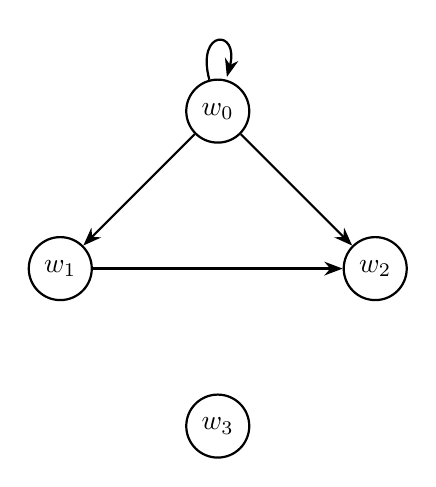
\begin{tikzpicture}[->, >=Stealth, thick, node distance=1.5cm, 
        main node/.style={circle,draw,minimum size=0.8cm}]
    \node[main node] (1) at (0,2) {$w_0$};
    \node[main node] (2) at (-2,0) {$w_1$};
    \node[main node] (3) at (2,0) {$w_2$};
    \node[main node] (4) at (0,-2) {$w_3$};

    \path[->]
        (1) edge[loop above] (1)
        (1) edge (2)
        (1) edge (3)
        (2) edge (3);
    \end{tikzpicture}
    }
    \end{center}

    \item \textbf{Example 2:}
    
    Consider the directed graph $G_2 = \langle V_2, E_2 \rangle$ with:


    \[V_2 = \{w_0, w_1, w_2, w_3\}, \quad E_2 = \{\langle w_0,w_1 \rangle, \langle w_1,w_2 \rangle, \langle w_2,w_3 \rangle, \langle w_3,w_0 \rangle\}\]

    \begin{center}
    \fbox{
    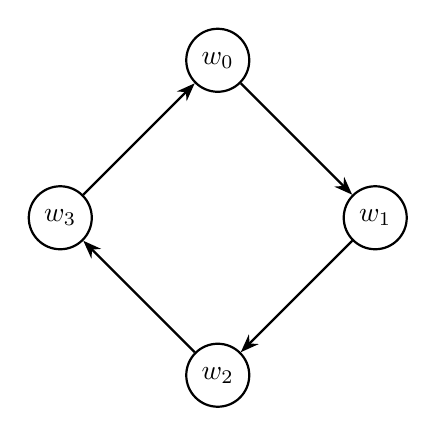
\begin{tikzpicture}[->, >=Stealth, thick, node distance=1.5cm, main node/.style={circle,draw,minimum size=0.8cm}]
    \node[main node] (1) at (0,2) {$w_0$};
    \node[main node] (2) at (2,0) {$w_1$};
    \node[main node] (3) at (0,-2) {$w_2$};
    \node[main node] (4) at (-2,0) {$w_3$};

    \path[->]
        (1) edge (2)
        (2) edge (3)
        (3) edge (4)
        (4) edge (1);
    \end{tikzpicture}
    }
    \end{center}

    \newpage

    \item \textbf{Example 3:}
    
    Consider the directed graph $G_3 = \langle V_3, E_3 \rangle$ with:

    \[
    V_3 = \{w_0, w_1, w_2, w_3, w_4\}, \quad E_3 = \{\langle w_0,w_1 \rangle, \langle w_0,w_2 \rangle, \langle w_1,w_3 \rangle, \langle w_2,w_3 \rangle, \langle w_3,w_4 \rangle\}
    \]

    \begin{center}
    \fbox{
    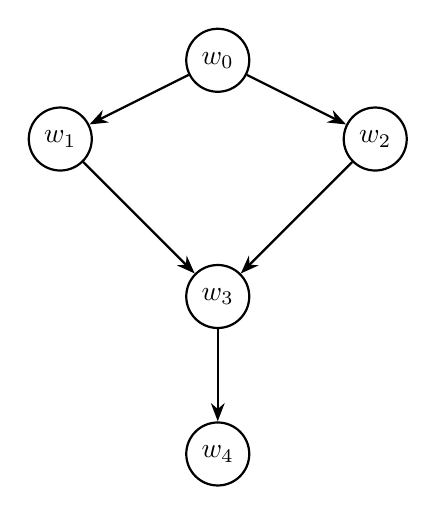
\begin{tikzpicture}[->, >=Stealth, thick, node distance=1.5cm, main node/.style={circle,draw,minimum size=0.8cm}]
    \node[main node] (1) at (0,2) {$w_0$};
    \node[main node] (2) at (-2,1) {$w_1$};
    \node[main node] (3) at (2,1) {$w_2$};
    \node[main node] (4) at (0,-1) {$w_3$};
    \node[main node] (5) at (0,-3) {$w_4$};

    \path[->]
        (1) edge (2)
        (1) edge (3)
        (2) edge (4)
        (3) edge (4)
        (4) edge (5);
    \end{tikzpicture}
    }
    \end{center}

    \item \textbf{Example 4:}
    
    Consider the directed graph $G_4 = \langle V_4, E_4 \rangle$ with:

    \[
    V_4 = \{w_0,w_1,w_2,w_3\}, \quad E_4 = \{\langle w_i,w_j \rangle \mid w_i,w_j \in V_4\}
    \]

    \begin{center}
    \fbox{
    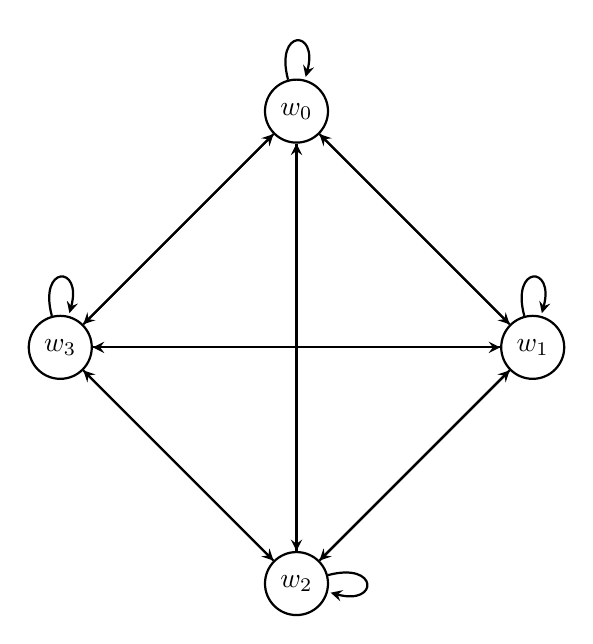
\begin{tikzpicture}[->,>=stealth,thick,node distance=1.5cm]
    \tikzstyle{vertex}=[circle,draw,minimum size=0.8cm]

    
    \node[vertex] (v1) at (90:3)  {$w_0$};
    \node[vertex] (v2) at (0:3)   {$w_1$};
    \node[vertex] (v3) at (-90:3) {$w_2$};
    \node[vertex] (v4) at (180:3) {$w_3$};

    
    \draw (v1) edge[loop above] (v1);
    \draw (v2) edge[loop above] (v2);
    \draw (v3) edge[loop right] (v3);   
    \draw (v4) edge[loop above] (v4);    

    
    \foreach \i in {1,...,4} {
        \foreach \j in {1,...,4} {
        \ifnum\i<\j
            \draw (v\i) -- (v\j);
            \draw (v\j) -- (v\i);
        \fi
        }
    }
    \end{tikzpicture}
    }
    \end{center}

    \newpage
    \item \textbf{Example 5:}
    
    
    Consider the directed graph $G_5 = \langle V_5, E_5 \rangle$ with:

    \[
    V_5 = \{w_0,w_1,w_2,w_3,w_4\}, \quad E_5 = \{\langle w_i,w_j \rangle \mid w_i,w_j \in V_5\}
    \]

    \begin{center}
    \fbox{
    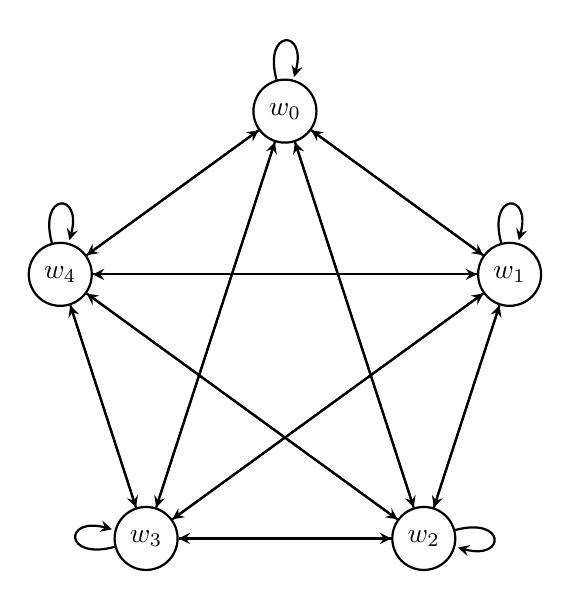
\begin{tikzpicture}[->,>=stealth,thick,node distance=1.5cm]
    \tikzstyle{vertex}=[circle,draw,minimum size=0.8cm]

    \node[vertex] (v1) at (90:3)   {$w_0$};
    \node[vertex] (v2) at (18:3)   {$w_1$};
    \node[vertex] (v3) at (-54:3)  {$w_2$};
    \node[vertex] (v4) at (-126:3) {$w_3$};
    \node[vertex] (v5) at (162:3)  {$w_4$};

    \draw (v1) edge[loop above] (v1);
    \draw (v2) edge[loop above] (v2);
    \draw (v3) edge[loop right] (v3);  
    \draw (v4) edge[loop left] (v4);    
    \draw (v5) edge[loop above] (v5);

    \foreach \i in {1,...,5} {
        \foreach \j in {1,...,5} {
        \ifnum\i<\j
            \draw (v\i) -- (v\j);
            \draw (v\j) -- (v\i);
        \fi
        }
    }
    \end{tikzpicture}
    }
    \end{center}

\end{enumerate}

\section{Operations on Relations}

Let $R, S \subseteq A^2$ be binary relations on a set $A$. The following are standard operations on relations:

\subsection{Inverse of a Relation}

Definition:

\[
R^{-1} = \{ \langle y, x \rangle \mid \langle x, y \rangle \in R \}
\]

In general, if $R \subseteq \mathbb{N}^2$, the inverse relation $R^{-1}$ contains all pairs of $R$ with their coordinates swapped:

\[
R^{-1} = \{ (y, x) \in \mathbb{N}^2 \mid (x, y) \in R \}
\]

\textbf{Example:}

Let \[S = \{ \langle x, y \rangle \in \mathbb{Z}^2 \mid x + 1 = y \}\]

that is,


\[
\begin{array}{c|ccccccc}
S & \cdots & -1 & 0 & 1 & 2 & 3 & \cdots \\
\hline
\vdots & \ddots & \vdots & \vdots & \vdots & \vdots & \vdots & \\
-1 & \cdots & & (-1,0) & & & & \cdots \\
0 & \cdots & & & (0,1) & & & \cdots \\
1 & \cdots & & & & (1,2) & & \cdots \\
2 & \cdots & & & & & (2,3) & \cdots \\
\vdots & & \vdots & \vdots & \vdots & \vdots & \vdots & \ddots \\
\end{array}
\]

then

\[
\begin{array}{c|ccccccc}
S^{-1} & \cdots & -2 & -1 & 0 & 1 & 2 & \cdots \\
\hline
\vdots & \ddots & \vdots & \vdots & \vdots & \vdots & \vdots & \\
0 & \cdots & & (0,-1) & & & & \cdots \\
1 & \cdots & & & (1,0) & & & \cdots \\
2 & \cdots & & & & (2,1) & & \cdots \\
3 & \cdots & & & & & (3,2) & \cdots \\
\vdots & & \vdots & \vdots & \vdots & \vdots & \vdots & \ddots \\
\end{array}
\]


\subsection{Relative Product of Relations}

Definition:

\[
(R \mid S) = \{ \langle x, z \rangle \mid \exists y \, (xRy \wedge ySz) \}
\]

\textbf{Example:}

Suppose we have 

\[
R = \{ (1, 2), (2, 3), (3, 4) \}, \quad
S = \{ (2, 5), (3, 6), (4, 7) \}
\]

Then the composition of relations is

\[
R \mid S = \{ (x, z) \mid \exists y \, ((x, y) \in R \wedge (y, z) \in S) \}
\]

Thus

\begin{enumerate}
\item $((1, 2) \in R) \text{ and } ((2, 5) \in S) \to ((1, 5) \in R \mid S)$ 
\item $((2, 3) \in R) \text{ and } ((3, 6) \in S) \to ((2, 6) \in R \mid S)$  
\item $((3, 4) \in R) \text{ and } ((4, 7) \in S) \to ((3, 7) \in R \mid S)$
\end{enumerate}

Consequently

\[
R \mid S = \{ (1, 5), (2, 6), (3, 7) \}
\]

\subsection{Restriction of a Relation}

Definition:

\[
R \upharpoonright A = R \cap A^2
\]

In general, if $R \subseteq \mathbb{N}^2$ and $A \subseteq \mathbb{N}$, the restriction of $R$ to $A$ keeps only those pairs in $R$ where both elements are in $A$:

\[
R \upharpoonright A = \{ (x, y) \in R \mid (x,y) \in A \}
\]

Hence

\[
\begin{array}{c|cccc}
A^2 & a_1 & a_2 & \dots & a_n \\
\hline
a_1 & (a_1,a_1) & (a_1,a_2) & \dots & (a_1,a_n) \\
a_2 & (a_2,a_1) & (a_2,a_2) & \dots & (a_2,a_n) \\
\vdots & \vdots & \vdots & \vdots & \vdots \\
a_n & (a_n,a_1) & (a_n,a_2) & \dots & (a_n,a_n) \\
\end{array}
\]

\textbf{Example 1:}

Given

\[R = \{(1, 2), (2, 4), (3, 6), (4, 8), (5, 10), (6, 12)\} \subseteq \mathbb{Z}^2\]

Restriction to even numbers $E = \{2, 4, 6, 8, 10, 12, \ldots\}$:

\[R \upharpoonright_E = \{(2, 4), (4, 8), (6, 12)\}\]


\textbf{Example 2:}

Given

\[f = \{(x, x^2) \mid x \in \mathbb{R}\}\]


Restriction to $\mathbb{Z} \cap [0,3]$:

\[
\begin{array}{c|cccc}
f \upharpoonright_{\mathbb{Z} \cap [0,3]} & 0 & 1 & 2 & 3 \\
\hline
0 & (0,0) & & & \\
1 & & (1,1) & & \\
2 & & & (2,4) & \\
3 & & & & (3,9) \\
\end{array}
\]

\textbf{Example 3:}

Let

\[
\begin{array}{c|ccccccc}
\mathbb{R}^2 & \cdots & a_{ijk} & \cdots & b_{lmn} & \cdots & c_{pqr} & \cdots \\
\hline
\vdots & \vdots & \vdots & \vdots & \vdots & \vdots & \vdots & \vdots \\
a_{ijk} & \cdots & (a_{ijk},a_{ijk}) & \cdots & (a_{ijk},b_{lmn}) & \cdots & (a_{ijk},c_{pqr}) & \cdots \\
\vdots & \vdots & \vdots & \vdots & \vdots & \vdots & \vdots & \vdots \\
b_{lmn} & \cdots & (b_{lmn},a_{ijk}) & \cdots & (b_{lmn},b_{lmn}) & \cdots & (b_{lmn},c_{pqr}) & \cdots \\
\vdots & \vdots & \vdots & \vdots & \vdots & \vdots & \vdots & \vdots \\
c_{pqr} & \cdots & (c_{pqr},a_{ijk}) & \cdots & (c_{pqr},b_{lmn}) & \cdots & (c_{pqr},c_{pqr}) & \cdots \\
\vdots & \vdots & \vdots & \vdots & \vdots & \vdots & \vdots & \vdots \\
\end{array}
\]

Restriction to $\mathbb{N}^2$:

\[
\begin{array}{c|cccc}
\mathbb{N}^2 & 1 & 2 & 3 & \cdots \\
\hline
1 & (1,1) & (1,2) & (1,3) & \cdots \\
2 & (2,1) & (2,2) & (2,3) & \cdots \\
3 & (3,1) & (3,2) & (3,3) & \cdots \\
\vdots & \vdots & \vdots & \vdots & \ddots \\
\end{array}
\]

Given relation

\[R = \{(a_{ijk}, c_{pqr}), (b_{lmn}, 2), (2, 3), (\pi, e), (3, 5)\} \subseteq \mathbb{R}^2\]

Restriction to $\mathbb{N}^2$:

\[R \upharpoonright_{\mathbb{N}^2} = \{(2, 3), (3, 5)\}\]

\subsection{Application of a Relation to a Set}

Definition:

\[
R[A] = \{ y \in A \mid \exists x \in A, \langle x, y \rangle \in R \}
\]

\textbf{Example:}

Let \[S = \{ (a,b), (b,c), (c,d) \}\]

and consider the set $P = \{a,b,c\}$.

Where

\[\begin{aligned}
   (a,b) &\to b \in S[\cdot]\\
    (b,c) &\to c \in S[\cdot]\\
    (c,d) &\to d \notin S[P] \text{ since } d \notin P
\end{aligned}
\]  

then

\[
S[P] = \{b,c\}
\]

\subsection{Transitive Closure}

Definition:

\[
R^1 = R, \quad R^{n+1} = R^n \mid R
\]

\[
R^+ = \displaystyle\bigcup_{n=1}^{\infty} R^n
\]

\textbf{Example:}

Let \[R = \{ (1,2), (2,3), (3,4) \}\] 

Since

\[\begin{aligned}
R^1 =& \{ (1,2), (2,3), (3,4) \} \\
R^2 =& R \mid R = \{ (1,3), (2,4) \} \\
R^3 =& R^2 \mid R = \{ (1,4) \}
\end{aligned}\]

Therefore

\[
\begin{array}{c|cccc}
R^+ & 1 & 2 & 3 & 4 \\
\hline
1 & & (1,2) & (1,3) & (1,4) \\
2 & & & (2,3) & (2,4) \\
3 & & & & (3,4) \\
4 & & & & \\
\end{array}
\]

\subsection{Reflexive Transitive Closure}


Let \[\text{Id}_A = \{ \langle x, x \rangle \mid x \in A \}\]

then

\[
R^* = R^+ \cup \text{Id}_A
\]

\textbf{Example:}

Since $\text{Id}_A$:

\[
\begin{array}{c|cccc}
\text{Id}_A & 1 & 2 & 3 & 4 \\
\hline
1 & (1,1) & & & \\
2 & & (2,2) & & \\
3 & & & (3,3) & \\
4 & & & & (4,4) \\
\end{array}
\]

We conclude that, $R^* = R^+ \cup \text{Id}_A$:

\[
\begin{array}{c|cccc}
R^* & 1 & 2 & 3 & 4 \\
\hline
1 & (1,1) & (1,2) & (1,3) & (1,4) \\
2 & & (2,2) & (2,3) & (2,4) \\
3 & & & (3,3) & (3,4) \\
4 & & & & (4,4) \\
\end{array}
\]

\section{Functions}

A function $f$ from set $A$ to set $B$ is a relation that assigns to each element of $A$ exactly one element of $B$.

Let $A$ and $B$ be sets. A function $f: A \to B$ is a subset $f \subseteq A \times B$ such that

\[
f = \{(x, y) \in A \times B \mid f(x) = y \}
\]

This is a subset of $A \times B$ such that for every $x \in A$, there exists a unique $y \in B$ with $(x, y) \in f$.

\subsection{Domain, Codomain, Range, and Preimage}

\begin{enumerate}
    \item Domain:
    \[
    \text{dom}(f) = A = \{x \mid \exists y \in B : (x, y) \in f\}
    \]

    \item Codomain:
    \[
    \text{cod}(f) = B
    \]

    \item Range (Image):
    \[
    \text{range}(f) = \text{im}(f) = \{y \in B \mid \exists x \in A : f(x) = y\}
    \]

    \item Image of a subset:
    
    For $S \subseteq A$:
    \[
    f(S) = \{f(x) \mid x \in S\} = \{y \in B \mid \exists x \in S : f(x) = y\}
    \]

    \item Preimage (Inverse Image):
    
    For $T \subseteq B$:
    \[
    f^{-1}(T) = \{x \in A \mid f(x) \in T\}
    \]
\end{enumerate}

\textbf{Example:}

Let 

\[
\begin{aligned} 
A &= \{1, 2, 3, 4, 5\}\\ 
B &= \{0, 1, 2, 3, 4, 5, 6, 7, 8, 9, 10\} 
\end{aligned}
\] 

Define 

\[
f: A \to B, \ f(x) = 2x
\] 

Let 

\[
S = \{1, 3, 5\} \subseteq A
\] 

Then 

\[
f(S) = \{f(x) \mid x \in S\}
\] 

\[
\begin{aligned} 
f(1) &= 2\\ 
f(3) &= 6\\ 
f(5) &= 10 
\end{aligned}
\] 

Therefore 

\[
\boxed{f(S) = \{2, 6, 10\}}
\]

\begin{enumerate}

    \item \textbf{Example 1:}

    Let $f : \mathbb{R} \to \mathbb{R}$ be defined by $f(x) = x^2$.

    \[
    \text{range}(f) = \{y \in \mathbb{R} \mid y \geq 0\} = [0, \infty)
    \]

    Image of a set:

    \[
    f(\{-2, 3\}) = \{(-2)^2, 3^2\} = \{4, 9\}
    \]

    Preimage of a set:

    \[
    f^{-1}(\{4\}) = \{x \in \mathbb{R} \mid x^2 = 4\} = \{-2, 2\}
    \]

    \item \textbf{Example 2:}

    Let

    \[
    \times : \mathbb{N} \times \mathbb{N} \to \mathbb{N}
    \]

    be the usual multiplication function defined by

    \[
    \times(a, b) = a \times b
    \]

    Then:

    \[
    \text{dom}(\times) = \mathbb{N} \times \mathbb{N}, \quad
    \text{cod}(\times) = \mathbb{N}, \quad
    \text{range}(\times) = \mathbb{N}
    \]

    For example:

    \[
    (3, 4) \in \mathbb{N} \times \mathbb{N}
    \]

    and

    \[
    3 \times 4 = 12
    \]

    Therefore,

    \[
    \times(3, 4) = 12
    \]

    We also have the identity property:

    \[
    \forall n \in \mathbb{N}, \; \exists (n, 1) \in \mathbb{N} \times \mathbb{N} : n \times 1 = n
    \]

    \item \textbf{Example 3:}

    Let
    \[
    f(x) = x^2 - 3x + 2
    \]

    We want to find

    \[
    f(2 + x)
    \]

    Substitute
    \[
    2 + x \ \text{for} \ x
    \]

    Hence

    \[
    f(2 + x) = (2 + x)^2 - 3(2 + x) + 2
    \]

    Expand and simplify:

    \[
    \begin{aligned}
    f(2 + x) &= (x^2 + 4x + 4) - 3(2 + x) + 2 \\
    &= x^2 + 4x + 4 - 6 - 3x + 2 \\
    &= x^2 + x
    \end{aligned}
    \]

    Thus,

    \[
    \boxed{f(2 + x) = x^2 + x}
    \]

    \item \textbf{Example 4:}

    Let
    \[
    f(x) = 2x + 3
    \]

    We want to find

    \[
    f^{-1}(x)
    \]

    we define

    \[
    \begin{aligned}
    y &= 2x + 3 \\
    y - 3 &= 2x \\
    x &= \frac{y - 3}{2}
    \end{aligned}
    \]

    Now, interchange
    \[
    x \ \text{and} \ y
    \]

    Hence:

    \[
    \boxed{f^{-1}(x) = \frac{x - 3}{2}}
    \]

    \item \textbf{Example 5:}

    Let 
    \[
    f : \mathbb{N} \to \mathbb{N}
    \]
    be defined by
    \[
    f(x) = x + 1
    \]

    Then:

    \[
    \text{range}(f) = \mathbb{Z}^+ = \{1, 2, 3, \ldots\}
    \]

    For example:
    \[
    f(0) = 1, \quad f(1) = 2, \quad f(2) = 3
    \]

    Hence,
    \[
    0 \notin \text{range}(f) \text{ since } \nexists x \in \mathbb{N} : f(x) = 0
    \]

    \item \textbf{Example 6:}

    Let $g : \mathbb{N} \to \mathbb{N}$ be defined by:

    \[
    g(x) = x + 2 - 1
    \]

    Then:

    \[
    \forall x \in \mathbb{N}, \; f(x) = x + 1 = x + 2 - 1 = g(x)
    \]

    By the principle of extensionality for functions:

    \[
    \forall x \in \text{dom}(f) : f(x) = g(x) \to f = g
    \]

    provided $\text{dom}(f) = \text{dom}(g)$ and $\text{cod}(f) = \text{cod}(g)$.

    \item \textbf{Example 7:}

    Let $h : \mathbb{N} \to \mathbb{N}$ be defined by:

    \[
    h(x) = \begin{cases}
    \displaystyle\frac{x}{2} & \text{if } x \text{ is even} \\[0.5em]
    \displaystyle\frac{x + 1}{2} & \text{if } x \text{ is odd}
    \end{cases}
    \]

    Since:

    \[
    \forall x \in \mathbb{N}, \; ( \text{even}(x) \lor \text{odd}(x))(x) \land \neg(\text{ even}(x) \land\text{odd}(x))
    \]

    the function $h$ is well-defined and $h(x) \in \mathbb{N}$ for all $x \in \mathbb{N}$.
\end{enumerate}

\newpage
\section{Kinds of Functions}

\subsection{Injective}

A function $f : A \to B$ is injective or one-to-one if and only if:

\[
\forall x_1, x_2 \in A,\ f(x_1) = f(x_2) \to x_1 = x_2.
\]

\begin{center}
\fbox{
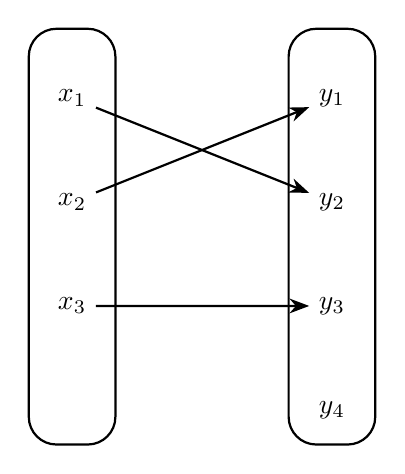
\begin{tikzpicture}[scale=1.1, every node/.style={scale=1}]

\draw[thick, rounded corners=10pt] (-0.5,-2.8) rectangle (0.5,2);

\draw[thick, rounded corners=10pt] (2.5,-2.8) rectangle (3.5,2);

\node (A1) at (0,1.2) {$x_1$};
\node (A2) at (0,0) {$x_2$};
\node (A3) at (0,-1.2) {$x_3$};

\node (B1) at (3,1.2) {$y_1$};
\node (B2) at (3,0) {$y_2$};
\node (B3) at (3,-1.2) {$y_3$};
\node (B4) at (3,-2.4) {$y_4$};

\draw[-{Stealth[length=2.5mm]}, thick] (A1) -- (B2);
\draw[-{Stealth[length=2.5mm]}, thick] (A2) -- (B1);
\draw[-{Stealth[length=2.5mm]}, thick] (A3) -- (B3);
\end{tikzpicture}
}
\end{center}

Equivalently, for each $y \in B$, there is at most one $x \in A$ such that $f(x) = y$.

We call such a function an injection from $A$ to $B$.

\begin{enumerate}
    \item \textbf{Example 1:}

    $f : \mathbb{R} \to \mathbb{R}$, where $f(x) = 2x + 3$

    If $2x_1 + 3 = 2x_2 + 3$, then $x_1 = x_2$.

    Exponential function is strictly increasing.

    \item \textbf{Example 2:}

    $f : \mathbb{Z} \to \mathbb{N}$, defined by

    \[
    f(x) =
    \begin{cases}
    2x, & \text{if } x \ge 0, \\
    -2x - 1, & \text{if } x < 0
    \end{cases}
    \]

    \item \textbf{Example 3:}

    There exist injective functions from $\mathbb{N}$ into each of $\mathbb{N}, \mathbb{Z}, \mathbb{Q}, \mathbb{R}$.
    Formally:
    \[
    \exists f_i : \mathbb{N} \to S_i, \quad S_i \in \{\mathbb{N}, \mathbb{Z}, \mathbb{Q}, \mathbb{R}\}, \text{ such that } f_i \text{ is injective.}
    \]

    \[
    \begin{aligned}
    f_1 &: \mathbb{N} \to \mathbb{N}, & f_1(x) &= x + 1 \\
    f_2 &: \mathbb{N} \to \mathbb{Z}, & 
    f_2(x) &=
    \displaystyle\begin{cases}
    \displaystyle\frac{x}{2}, & \text{if } x \text{ is even} \\
    -\displaystyle\frac{x+1}{2}, & \text{if } x \text{ is odd}
    \end{cases} \\
    f_3 &: \mathbb{N} \to \mathbb{Q}, & f_3(x) &= \displaystyle\frac{x}{x+1} \\
    f_4 &: \mathbb{N} \to \mathbb{R}, & f_4(x) &= x.
    \end{aligned}
    \]

    Each $f_i$ is injective, since distinct natural numbers map to distinct elements of the codomain.

    \item \textbf{Example 4:}

    Let  
    
    \[
    f: \{2n+1 \mid n \in \mathbb{N}\} \longrightarrow \mathbb{Q}, \quad f(2n+1) = \displaystyle\frac{2n+1}{2n+2}
    \]

    \[
    \displaystyle\operatorname{Im}(f) = \left\{\, \frac{a}{b} \in \mathbb{Q} \;\middle|\; a \in \{2n+1 \mid n \in \mathbb{N}\},\ b = a+1 \,\right\}
    \]

    Hence,

    \[
    \begin{aligned}
    f(1)= & \ 1/2 \\
    f(3)= & \ 3/4 \\
    f(5)= & \ 5/6 \\
    f(7)= & \ 7/8 \\
    f(9)= & \ 9/10 \\
    \vdots
    \end{aligned}
    \]
\end{enumerate}

\subsection{Surjective}

A function $f : A \to B$ is surjective or onto if and only if $B$ is the range of $f$, i.e.,

\[
\forall y \in B,\ \exists x \in A \mid f(x) = y.
\]

\begin{center}
\fbox{
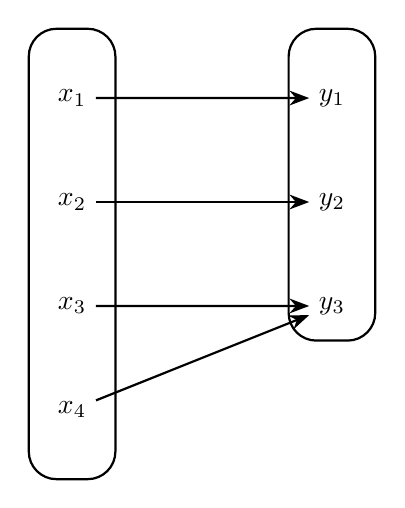
\begin{tikzpicture}[scale=1.1, every node/.style={scale=1}]

\draw[thick, rounded corners=10pt] (-0.5,-3.2) rectangle (0.5,2);

\draw[thick, rounded corners=10pt] (2.5,-1.6) rectangle (3.5,2);

\node (A1) at (0,1.2) {$x_1$};
\node (A2) at (0,0) {$x_2$};
\node (A3) at (0,-1.2) {$x_3$};
\node (A4) at (0,-2.4) {$x_4$};

\node (B1) at (3,1.2) {$y_1$};
\node (B2) at (3,0) {$y_2$};
\node (B3) at (3,-1.2) {$y_3$};

\draw[-{Stealth[length=2.5mm]}, thick] (A1) -- (B1);
\draw[-{Stealth[length=2.5mm]}, thick] (A2) -- (B2);
\draw[-{Stealth[length=2.5mm]}, thick] (A3) -- (B3);
\draw[-{Stealth[length=2.5mm]}, thick] (A4) -- (B3);
\end{tikzpicture}
}
\end{center}

We call such a function a surjection from $A$ to $B$.

\begin{enumerate}
    \item \textbf{Example 1:}

    $f : \mathbb{Z} \to \mathbb{N}$, where $f(x) = |x|$

    \[
    \begin{array}{c|ccccccc}
    x & -3 & -2 & -1 & 0 & 1 & 2 & 3 \\ \hline
    |x| & 3 & 2 & 1 & 0 & 1 & 2 & 3
    \end{array}
    \]

    \item \textbf{Example 2:}

    $f : \mathbb{R} \to \mathbb{R}$, where $f(x) = x^3$

    \[
    \forall y \in \mathbb{R}, \exists x = \sqrt[3]{y} \in \mathbb{R} \mid f(x) = y
    \]

    \item \textbf{Example 3:}

    $f : \mathbb{R} \to [0, \infty)$, where $f(x) = x^2$

    \[
    f(\sqrt{x}) = (\sqrt{x})^2 = x
    \]

    \item \textbf{Example 4:}

    Floor function: $f : \mathbb{R} \to \mathbb{Z}$, where $f(x) = \lfloor x \rfloor$

    \[
    \begin{array}{c|ccccc}
    x & -2.7 & -1.2 & 0.5 & 1.0 & 2.9 \\ \hline
    \lfloor x \rfloor & -3 & -2 & 0 & 1 & 2
    \end{array}
    \]
\end{enumerate}

\subsection{Bijective}

A function $f : A \to B$ is bijective if and only if it is both injective and surjective. We call such a function a bijection from $A$ to $B$, or a one-to-one correspondence.

Equivalently:

\[
\forall y \in B,\ \exists! x \in A \mid f(x) = y.
\]

\begin{center}
\fbox{
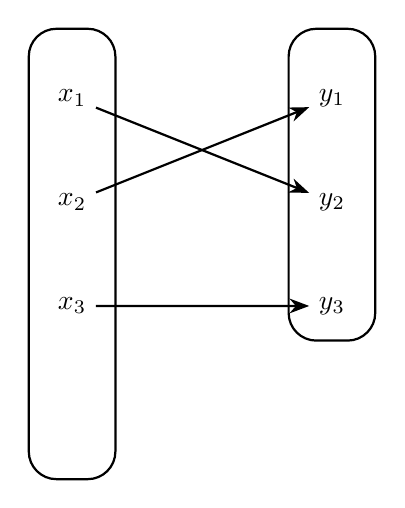
\begin{tikzpicture}[scale=1.1, every node/.style={scale=1}]
\draw[thick, rounded corners=10pt] (-0.5,-3.2) rectangle (0.5,2);
\draw[thick, rounded corners=10pt] (2.5,-1.6) rectangle (3.5,2);
\node (A1) at (0,1.2) {$x_1$};
\node (A2) at (0,0) {$x_2$};
\node (A3) at (0,-1.2) {$x_3$};
\node (B1) at (3,1.2) {$y_1$};
\node (B2) at (3,0) {$y_2$};
\node (B3) at (3,-1.2) {$y_3$};
\draw[-{Stealth[length=2.5mm]}, thick] (A1) -- (B2);
\draw[-{Stealth[length=2.5mm]}, thick] (A2) -- (B1);
\draw[-{Stealth[length=2.5mm]}, thick] (A3) -- (B3);
\end{tikzpicture}
}
\end{center}

(For every element in $B$, there exists exactly one element in $A$ that maps to it.)

\begin{enumerate}
    \item \textbf{Example:}

    Let

    \[
    A = \{1, 2, 3\}, \quad B = \{a, b, c\}.
    \]

    Define a function

    \[
    f : A \to B
    \]
    
    by
    
    \[
    f(1) = a, \quad f(2) = b, \quad f(3) = c.
    \]

    Each element of $A$ maps to a unique element of $B$, so $f$ is injective. Every element of $B$ is the image of some element of $A$, so $f$ is surjective. Therefore, $f$ is bijective.
\end{enumerate}

\subsection{Combinations}

\subsubsection{Bijective (Both injective and surjective)}

\begin{enumerate}
    \item \textbf{Example 1:}

    Identity function: $f : \mathbb{R} \to \mathbb{R}$, where $f(x) = x$

    Injective and surjective, therefore bijective:
    
    \[
    \forall y \in \mathbb{R}, \exists! x \in \mathbb{R} \mid f(x) = y
    \]

    \item \textbf{Example 2:}

    $f : [0, \infty) \to [0, \infty)$, where $f(x) = x^2$

    Injective: 
    
    \[
    \forall x_1, x_2 \in [0, \infty), x_1^2 = x_2^2 \Longrightarrow x_1 = x_2
    \]

    Surjective: 
    
    \[
    \forall y \in [0, \infty), \exists x \in [0, \infty) \mid f(x) = y
    \]

    Therefore bijective.
\end{enumerate}

\subsubsection{Injective but not surjective}

Recall the Von Neumann Ordinal, 

\[
\begin{aligned}
   0 &= \varnothing = \{\}\\
   1 &= \{\varnothing\} = \varnothing \cup \{\varnothing\}\\
   2 &= \{\varnothing, \{\varnothing\}\} = 1 \cup \{1\}\\
   &\vdots\\
   n &= n-1 \cup \{n-1\}
\end{aligned}
\]

Based on this notion, we can define a function that is injective but not surjective:

\begin{enumerate}
    \item \textbf{Example:}

    Let $A = \{1, 2, 3\}$ and define $f: A \to \mathcal{P}(A)$ by $F(x) = \{x\}$.

    Then:
    
    \[
    f(1) = \{1\}, \quad f(2) = \{2\}, \quad f(3) = \{3\}
    \]

    Hence:
    
    \[
    \operatorname{Im}(f) = \{\{1\}, \{2\}, \{3\}\} \subset \mathcal{P}(A)
    \]

    Since $\varnothing \in \mathcal{P}(A)$ but $\varnothing \notin \operatorname{Im}(f)$, we conclude that $f$ is injective but not surjective
\end{enumerate}

\subsubsection{Surjective but not injective}

\begin{enumerate}
    \item \textbf{Example:}

    Piecewise function: $f : \mathbb{N} \to \mathbb{N}$, where
    
    \[
    f(x) = \begin{cases} \displaystyle\frac{x}{2} & \text{if } x \text{ is even} \\ \displaystyle\frac{x+1}{2} & \text{if } x \text{ is odd} \end{cases}
    \]

    Surjective: 
    
    \[
    \forall y \in \mathbb{N}, \exists x \in \mathbb{N} : f(x) = y
    \]

    Not injective: 
    
    \[
    f(1) = f(2) = 1 \text{ but } 1 \neq 2
    \]
\end{enumerate}

\subsubsection{Neither injective nor surjective}

\begin{enumerate}
    \item \textbf{Example 1:}

    Constant function: $f : \mathbb{N} \to \mathbb{N}$, where $f(x) = 1$ for all $x$

    Not injective: 
    
    \[
    f(1) = f(2) = 1 \text{ but } 1 \neq 2
    \]

    Not surjective: 
    
    \[
    \nexists x \in \mathbb{N} \mid f(x) = 2
    \]

    \item \textbf{Example 2:}

    $f : \mathbb{R} \to \mathbb{R}$, where $f(x) = x^2$

    Not injective: 
    
    \[
    f(-2) = f(2) = 4 \text{ but } -2 \neq 2
    \]

    Not surjective: 
    
    \[
    \nexists x \in \mathbb{R} \mid f(x) = -1
    \]
\end{enumerate}

\subsection{Equivalence Relation with Function Properties}

\begin{enumerate}
    \item \textbf{Example 1:}

    Let $E = \{a, b, c, d, e, f\}$. Define $R \subseteq E^2$:

    \[
    \begin{array}{c|cccccc}
    R & a & b & c & d & e & f \\
    \hline
    a & (a,a) & (a,b) &  &  &  &  \\
    b & (b,a) & (b,b) &  &  &  &  \\
    c &  &  & (c,c) & (c,d) &  &  \\
    d &  &  & (d,c) & (d,d) &  &  \\
    e &  &  &  &  & (e,e) & (e,f) \\
    f &  &  &  &  & (f,e) & (f,f) \\
    \end{array}
    \]

    Reflexive:

    \[
    \forall x \in E,\ (x,x) \in R
    \]

    Symmetric:

    \[
    \forall x,y \in E,\ (x,y) \in R \to (y,x) \in R
    \]

    Transitive:

    \[
    \forall x,y,z \in E,\ (x,y) \in R \wedge (y,z) \in R \to (x,z) \in R
    \]

    Equivalence classes:

    \[
    [a] = \{a,b\}, \quad [c] = \{c,d\}, \quad [e] = \{e,f\}
    \]

    Thus:
    
    \[
    E/R = \{[a], [c], [e]\}
    \]

    Function $f: E \to E/R$

    Defined by:
    
    \[
    f(x) = [x]
    \]

    Not injective:

    \[
    a \ne b \ \wedge\ f(a) = f(b) 
    \]

    Surjective:

    \[
    \forall y \in E/R,\ \exists x \in E: f(x) = y 
    \]

    Not bijective:

    \[
    \neg \text{Injective} \to \neg \text{Bijective}
    \]

    Therefore:

    \[
    E \not\cong E/R
    \]

    Bijective Function Defined on Quotient Classes

    Let:
    
    \[
    S = \{a,c,e\}
    \]

    Define:

    \[
    g: E/R \to S,\quad g([a]) = a,\ g([c]) = c,\ g([e]) = e
    \]

    Injective:

    \[
    \forall x_1,x_2 \in E/R,\ g(x_1) = g(x_2) \to x_1 = x_2
    \]

    Surjective:
    
    \[
    \forall y \in S,\ \exists x \in E/R,\ g(x) = y
    \]

    Bijective:

    \[
    \text{Injective} \wedge \text{Surjective} \to \text{Bijective}
    \]

    Therefore:
    
    \[
    E/R \cong Sd
    \]

    \item \textbf{Example 2:}

    Let $X = \mathbb{N}^2$. Define $R \subseteq X^2$ by:
    
    \[
    (x_1,y_1) \,R\, (x_2,y_2) \leftrightarrow x_1 + y_2 = y_1 + x_2
    \]

    By definition of equivalence:

    Reflexive:
    
    \[
    \forall (x,y) \in X, \; (x,y) \,R\, (x,y)
    \]

    Symmetric:
    
    \[
    \forall (x_1,y_1),(x_2,y_2) \in X, \; ((x_1,y_1) \,R\, (x_2,y_2) \to (x_2,y_2) \,R\, (x_1,y_1))
    \]

    Transitive:
    
    \[
    \forall (x_1,y_1),(x_2,y_2),(x_3,y_3) \in X, \; ((x_1,y_1) \,R\, (x_2,y_2) \wedge (x_2,y_2) \,R\, (x_3,y_3) \to (x_1,y_1) \,R\, (x_3,y_3))
    \]

    Equivalence Classes:
    
    \[
    [(x_1,y_1)] = \{(x_2,y_2) : x_2 - y_2 = x_1 - y_1\}
    \]

    Quotient set:
    
    \[
    X/R = \{[(x,y)] : (x,y) \in \mathbb{N}^2\}
    \]

    Define:
    
    \[
    \Sigma: X/R \to \mathbb{Z}, \quad \Sigma([(x,y)]) = x - y
    \]

    Values:
    
    \[
    \begin{array}{c|ccccc}
    \Sigma(x,y) & 1 & 2 & 3 & 4 & 5 \\
    \hline
    1 & 0 & -1 & -2 & -3 & -4 \\
    2 & 1 & 0 & -1 & -2 & -3 \\
    3 & 2 & 1 & 0 & -1 & -2 \\
    4 & 3 & 2 & 1 & 0 & -1 \\
    5 & 4 & 3 & 2 & 1 & 0 \\
    \end{array}
    \]

    Injective
    
    \[
    \Sigma([(x_1,y_1)]) = \Sigma([(x_2,y_2)]) \to x_1 - y_1 = x_2 - y_2 \to (x_1,y_1) \,R\, (x_2,y_2) \to [(x_1,y_1)] = [(x_2,y_2)]
    \]

    \[
    \begin{array}{c|cccccc}
    \Sigma([(x,y)]) & -2 & -1 & 0 & 1 & 2 & \dots\\
    \hline
    \text{Pairs } & (0,2) & (0,1) & (0,0) & (1,0) & (2,0) & \dots \\
    \vdots & \vdots & \vdots & \vdots & \vdots & \vdots & \ddots
    \end{array}
    \]

    Surjective
    
    \[
    \forall z \in \mathbb{Z}, \; \exists (x,y) \in \mathbb{N}^2, \; \Sigma([(x,y)]) = z
    \]

    \[
    \begin{array}{c|cccccc}
    z \in \mathbb{Z} & -2 & -1 & 0 & 1 & 2 & \dots\\
    \hline
    \text{Pair } & (0,2) & (0,1) & (0,0) & (1,0) & (2,0) & \dots \\
    \vdots & \vdots & \vdots & \vdots & \vdots & \vdots & \ddots
    \end{array}
    \]

    Bijective
    
    \[
    \text{Injective} \wedge \text{Surjective} \to \text{Bijective}
    \]

    We conclude that:
    
    \[
    X/R \cong \mathbb{Z}
    \]
\end{enumerate}

\section{Functions as Relations}

A function $f: A \to B$ defines a relation between $A$ and $B$:

\[
x \in A \ R \ y \in B \leftrightarrow f(x) = y
\]

We identify $f$ with its set of ordered pairs:

\[
f = \{(x, y) \mid x \in A \land f(x) = y\} \subseteq A \times B
\]

\subsection{Graph of a Function}

Let $R \subseteq A \times B$ satisfy:

\[
(xRy \land xRz) \to y = z, \quad \text{and} \quad \forall x \in A, \exists y \in B \mid \langle x, y \rangle \in R.
\]

Then $R$ is the graph of a function $f : A \to B$ defined by $f(x) = y \leftrightarrow xRy$.

Let $f : A \to B$ be a function. The graph of $f$ is the relation $R_f \subseteq A \times B$ defined by:

\[
R_f = \{ \langle x, y \rangle \mid f(x) = y \}.
\]

\begin{enumerate}
    \item \textbf{Example 1:}

    Define a function $f : \mathbb{N} \to \mathbb{Z}$ by
    
    \[
    f(n) = (-1)^n \cdot \left\lfloor \displaystyle\frac{n+1}{2} \right\rfloor
    \]

    Explicitly:
    
    \[
    \begin{aligned}
    n = 0: & \quad \left\lfloor \frac{0+1}{2} \right\rfloor = \left\lfloor 0.5 \right\rfloor = 0 \to f(0) = (-1)^0 \cdot 0 = 0 \\
    n = 1: & \quad \left\lfloor \frac{1+1}{2} \right\rfloor = \left\lfloor 1 \right\rfloor = 1 \to f(1) = (-1)^1 \cdot 1 = -1 \\
    n = 2: & \quad \left\lfloor \frac{2+1}{2} \right\rfloor = \left\lfloor 1.5 \right\rfloor = 1 \to f(2) = (-1)^2 \cdot 1 = 1 \\
    n = 3: & \quad \left\lfloor \frac{3+1}{2} \right\rfloor = \left\lfloor 2 \right\rfloor = 2 \to f(3) = (-1)^3 \cdot 2 = -2 \\
    n = 4: & \quad \left\lfloor \frac{4+1}{2} \right\rfloor = \left\lfloor 2.5 \right\rfloor = 2 \to f(4) = (-1)^4 \cdot 2 = 2
    \end{aligned}
    \]

    Therefore: $f(0) = 0, \quad f(1) = -1, \quad f(2) = 1, \quad f(3) = -2, \quad f(4) = 2, \ldots$

    Then the graph is:

    \[
    R_f = \{(0,0), (1,-1), (2,1), (3,-2), (4,2), \ldots\}
    \]

    Each element in $\mathbb{N}$ maps to exactly one element in $\mathbb{Z}$.

    \item \textbf{Example 2:}

    Let
    
    \[
    A = \{a_i \mid i \ge 1\},\qquad
    B = \{b_k \mid k \ge 1\},\qquad
    C = \{c_j \mid j \ge 1\}.
    \]

    Define functions
    
    \[
    f:A\to B,\qquad f(a_i)=b_i \quad\forall i\ge1,
    \]
    
    \[
    g:B\to C,\qquad g(b_k)=c_k \quad\forall k\ge1.
    \]

    Their graphs are
    
    \[
    \begin{aligned}
    R_f &= \{(a_i,b_i)\mid i\ge1\},\\
    R_g &= \{(b_k,c_k)\mid k\ge1\}.
    \end{aligned}
    \]

    \begin{enumerate}
        \item Relational composition
        
        \[
        R_f\mid R_g
        \]

        Take an arbitrary pair
        
        \[
        (a_i,c_j)\in R_f\mid R_g.
        \]

        By definition of relational composition, there exists some index $k$ such that
        
        \[
        (a_i,b_k)\in R_f \ \land \  (b_k,c_j)\in R_g.
        \]

        Because
        
        \[
        R_f = \{(a_i,b_i)\mid i\ge1\},
        \]
        
        the only pair whose first component is $a_i$ is $(a_i,b_i)$. Thus
        
        \[
        b_k = b_i \to k=i.
        \]

        Similarly, since
        
        \[
        R_g = \{(b_k,c_k)\mid k\ge1\},
        \]
        
        then
        
        \[
        c_j = c_k \to j=k.
        \]

        Therefore,
        
        \[
        j = k = i,
        \]
        
        which implies
        
        \[
        R_f \mid R_g = \{(a_i,c_i)\mid i\ge1\}.
        \]

        \item Function composition

        \[
        g\circ f
        \]

        For each $i\ge1$,
        
        \[
        (g\circ f)(a_i)=g(f(a_i))=g(b_i)=c_i,
        \]
        
        so the graph of the composite is
        
        \[
        R_{g\circ f} = \{(a_i,c_i)\mid i\ge1\}.
        \]
    \end{enumerate}

    Thus,
    
    \[
    \boxed{R_f\mid R_g = R_{g\circ f} = \{(a_i,c_i)\mid i\ge1\}.}
    \]
\end{enumerate}

\subsection{Restriction and Image}

Let $f : A \to B$ be a function and let $C \subseteq A$. The restriction of $f$ to $C$, denoted $f\!\restriction C : C \to B$, 
is defined by

\[
(f\!\restriction C)(x) = f(x), \forall x \in C.
\]

Equivalently, in terms of graphs:

\[
R_{f\!\restriction C} 
= \{ (x, y) \in R_f \mid x \in C \}.
\]

The image of $C$ under $f$ is:

\[
f[C] = \{ f(x) \mid x \in C \}.
\]

\begin{enumerate}
    \item \textbf{Example 1:}

    Let $f : \mathbb{R} \to \mathbb{R}$ be defined by
    
    \[
    f(x) = x^2.
    \]

    Let $C = [0,\infty) \subseteq \mathbb{R}$.
    The restriction of $f$ to $C$ is the function
    
    \[
    f\!\restriction C : C \to \mathbb{R},
    \]
    
    defined by
    
    \[
    (f\!\restriction C)(x) = x^2 \quad \forall x \in C.
    \]

    The graph of $f$ is
    
    \[
    R_f = \{ (x, x^2) \mid x \in \mathbb{R} \}.
    \]

    The graph of the restricted function is

    \[
    R_{f\!\restriction C}
    = \displaystyle\bigcup_{x \in [0,\infty)} \{ (x, x^2) \}.
    \]

    \item \textbf{Example 2:}

    Let $f : \mathbb{N} \to \mathbb{Z}$ be defined by
    
    \[
    f(n) = (-1)^n \cdot n.
    \]

    Let $\mathbb{P}$ be the set of prime numbers:
    
    \[
    \mathbb{P} = \{2, 3, 5, 7, 11, \dots\} \subseteq \mathbb{N}.
    \]

    The restriction of $f$ to $\mathbb{P}$ is the function
    
    \[
    f\!\restriction \mathbb{P} :\mathbb{P} \to \mathbb{Z},
    \]
    
    defined by

    \[
    (f\!\restriction \mathbb{P})(p) = (-1)^p \cdot p
    \quad \forall p \in \mathbb{P}.
    \]

    The graph of $f$ is
    
    \[
    R_f = \{ (n, (-1)^n \cdot n ) \mid n \in \mathbb{N} \}.
    \]

    The graph of the restricted function is

    \[
    R_{f\!\restriction \mathbb{P}}
    = \displaystyle\bigcup_{p \in \mathbb{P}} \{ (p, (-1)^p \cdot p ) \}.
    \]
\end{enumerate}

\subsection{Composition of Functions}

Let $f: A \to B$ and $g: B \to C$ be functions. The \emph{composition} of $f$ and $g$, denoted $g \circ f$, is the function:

\[
(g \circ f): A \to C
\]

defined by:

\[
(g \circ f)(x) = g(f(x)), \forall x \in A
\]

This operation is only defined when the range of $f$ is a subset of the domain of $g$.

\begin{enumerate}
    \item \textbf{Example 1:}

    Consider two functions:

    \[
    f(x) = x + 1, \quad g(x) = 2x
    \]

    To compute $(g \circ f)(x)$:

    \[
    \begin{aligned}
    (g \circ f)(x) &= g(f(x)) \\
    &= g(x + 1) \\
    &= 2(x + 1) \\
    &= 2x + 2
    \end{aligned}
    \]

    So the composed function is:

    \[
    (g \circ f)(x) = 2x + 2
    \]

    \item \textbf{Example 2:}

    Consider two functions:

    \[
    f: \mathbb{N} \to \mathbb{Z}, \quad f(n) = 2n - 5
    \]

    \[
    g: \mathbb{Z} \to \mathbb{Q}, \quad g(z) = \displaystyle\frac{z + 1}{3}
    \]

    To compute $(g \circ f)(n)$:

    \[
    \begin{aligned}
    (g \circ f)(n) &= g(f(n)) \\
    &= g(2n - 5) \\
    &= \displaystyle\frac{(2n - 5) + 1}{3} \\
    &= \displaystyle\frac{2n - 4}{3}
    \end{aligned}
    \]

    So the composed function is:

    \[
    (g \circ f): \mathbb{N} \to \mathbb{Q}, \quad (g \circ f)(n) = \displaystyle\frac{2n - 4}{3}
    \]

    \item \textbf{Example 3:}

    Let

    \[
    f(x) = x + 1, \quad g(x) = 2x
    \]

    Then:

    \[
    (g \circ f)(x) = g(f(x)) = 2(x + 1) = 2x + 2
    \]

    \[
    (f \circ g)(x) = f(g(x)) = (2x) + 1 = 2x + 1
    \]
\end{enumerate}

\subsection{Partial Function}

A partial function $f : A \rightharpoonup B$ is a mapping that assigns to every element of $A$ \emph{at most one} element of $B$.

\begin{enumerate}
    \item If $f$ assigns a value to $x \in A$, we say $f(x)$ is defined, and write $f(x) \downarrow$.
    \item Otherwise, $f(x)$ is undefined, and we write $f(x) \uparrow$.
    \item The domain of a partial function $f$ is:

    \[
    \text{dom}(f) = \{x \in A : f(x) \downarrow\}
    \]
\end{enumerate}

\begin{enumerate}
    \item \textbf{Example 1:}

    Every total function $f : A \to B$ is also a partial function where $\text{dom}(f) = A$.

    Let $A = \{1, 2, 3\}$ and $B = \{a, b, c\}$. Define a function $f : A \to B$ by:

    \[
    f(1) = a, \quad f(2) = b, \quad f(3) = c
    \]

    This function is total, since every element of $A$ is assigned an element of $B$. We can also view it as a partial function:

    \[
    f : A \rightharpoonup B \quad \text{with } \text{dom}(f) = A
    \]

    This illustrates that a total function is just a special case of a partial function where the function is defined for all inputs.

    \item \textbf{Example 2:}

    Let $f : \mathbb{R} \rightharpoonup \mathbb{R}$ be defined by:

    \[
    f(x) = \displaystyle\frac{1}{x}
    \]

    Then $f$ is undefined at $x = 0$:

    \[
    f(0) \uparrow \quad \text{but} \quad f(x) \downarrow \text{ for } x \in \mathbb{R} \setminus \{0\}
    \]

    The function $f$ is defined on all real numbers except $0$. So the domain of $f$ is:

    \[
    \text{dom}(f) = \mathbb{R} \setminus \{0\}
    \]

    \item \textbf{Example 3:}

    Define $g : \mathbb{N} \rightharpoonup [0, 1]$ by:

    \[
    g(n) = \begin{cases}
    \dfrac{1}{2^n} & n \text{ even}, \\[1em]
    \text{$\uparrow$} & n \text{ odd.}
    \end{cases}
    \]

    This is a partial function because $g(n)$ is undefined for all odd natural numbers. Here $\text{dom}(g) = \{0, 2, 4, 6, ...\} \subset \mathbb{N}$.
\end{enumerate}

\subsection{Graph of a Partial Function}

The graph of a partial function $f : A \rightharpoonup B$ is the set:

\[
R_f = \{(x, y) \in A \times B \mid f(x) = y\}
\]

Let $R \subseteq A \times B$ satisfy:

\[
\forall x \in A, \forall y, y' \in B, \, (x, y) \in R \land (x, y') \in R \to y = y'
\]

Then $R$ is the graph of a partial function $f : A \rightharpoonup B$, defined by:

\[
f(x) = \begin{cases} y & \text{if } (x, y) \in R, \exists y \in B \\ \uparrow & \text{otherwise} \end{cases}
\]

If in addition, $R$ is serial, i.e., $\forall x \in A, \exists y \in B \mid (x, y) \in R$, then $f$ is a total function.

\textbf{Example:}

Let $A = \{1, 2, 3, 4\}$ and $B = \{a, b\}$.

Define a relation $R \subseteq A \times B$ by:

\[
R = \{(1, a), (2, a), (4, b)\}
\]

This satisfies:

\[
\forall x \in A, \forall y, y' \in B, \, (x, y) \in R \land (x, y') \in R \to y = y'
\]

So $R$ is the graph of a partial function $f : A \rightharpoonup B$, where:

\[
f(1) = a,\quad f(2) = a,\quad f(4) = b,\quad f(3) \uparrow
\]

\section{Inverses of Functions}

A function $g : Y \to X$ is an inverse of a function $f : X \to Y$ if

\[
f(g(y)) = y  \land  g(f(x)) = x,\quad \forall  x, \forall y \ (x \in X \land y \in Y)
\]

\textbf{Example:}

Let  

\[
f(x) = a x + b, \qquad g(y) = \displaystyle\frac{y - b}{a}.
\]

Then we can verify that

\[
f(g(y)) = a \displaystyle\left( \frac{y - b}{a} \right) + b = y,
\]

and

\[
g(f(x)) = \displaystyle\frac{(a x + b) - b}{a} = x.
\]

Therefore,  $g$ is the inverse of $f$.

\subsection{Left and Right Inverse}

Let $f : X \to Y$

\begin{enumerate}
    \item A function $g : Y \to X$ is a left inverse of $f$ if $g(f(x)) = x$,  $\forall x \in X$.

    \[
    X \xrightarrow{\,f\,} Y \xrightarrow{\,g\,} X
    \]

    The condition is:
    
    \[
    g(f(x)) = x, \quad \forall x \in X.
    \]

    Logical implication:
    
    \[
    (\exists g : Y \to X)\,[g \circ f = \mathrm{id}_X]
    \;\leftrightarrow\;
    f \text{ is injective}.
    \]

    \textbf{Example:}

    Let
    
    \[
    f: [0, \infty) \to \mathbb{R}, \
    f(x) = a^x, \ a > 0,\, a \ne 1.
    \]

    Define 
    
    \[
    g(y) = \log_a(y).
    \]

    Then
    
    \[
    g(f(x)) = \log_a(a^x) = x,
    \]

    so $g$ is a left inverse of $f$.

    \item A function $h : Y \to X$ is a right inverse of $f$ if $f(h(y)) = y$,  $\forall y \in Y$.

    \[
    Y \xrightarrow{\,h\,} X \xrightarrow{\,f\,} Y
    \]

    The condition is:
    
    \[
    f(h(y)) = y, \quad \forall y \in Y.
    \]

    Logical implication:
    
    \[
    (\exists h : Y \to X)\,[f \circ h = \mathrm{id}_Y]
    \;\leftrightarrow\;
    f \text{ is surjective}.
    \]

    \textbf{Example:}

    Let
    
    \[
    f: [0, \infty) \to \mathbb{R}, \
    f(x) = x^2.
    \]

    Define
    
    \[
    h(y) = \sqrt{y}.
    \]

    Then
    
    \[
    f(h(y)) = (\sqrt{y})^2 = y,
    \]
    
    so $h$ is a right inverse of $f$.

    \item Two-Sided Inverse

    \[
    X \overset{f}{\underset{f^{-1}}{\leftrightarrow}} Y
    \]

    The conditions are:
    
    \[
    f(f^{-1}(y)) = y, \quad f^{-1}(f(x)) = x.
    \]

    Logical implication:
    
    \[
    f \text{ is bijective}, \quad f^{-1} \text{ is unique}.
    \]

    \textbf{Example:}

    Let
    
    \[
    \mathbb{N} = \{1,2,3,4,\ldots\}, 
    \quad
    \mathbb{Z} = \{\ldots,-2,-1,0,1,2,\ldots\}.
    \]

    Define a bijection $f : \mathbb{N} \to \mathbb{Z}$:

    \[
    f(n) = 
    \begin{cases}
    \displaystyle\frac{n}{2}, & \text{if } n \text{ is even} \\[6pt]
    -\displaystyle\frac{n-1}{2}, & \text{if } n \text{ is odd}
    \end{cases}
    \]

    Define its inverse $f^{-1} : \mathbb{Z} \to \mathbb{N}$:

    \[
    f^{-1}(z) = 
    \begin{cases}
    2z, & \text{if } z > 0 \\[6pt]
    1, & \text{if } z = 0 \\[6pt]
    -2z + 1, & \text{if } z < 0
    \end{cases}
    \]

    Left inverse condition:
    
    \[
    f^{-1}(f(n)) = n, \quad \forall n \in \mathbb{N}.
    \]

    Right inverse condition:
    
    \[
    f(f^{-1}(z)) = z, \quad \forall z \in \mathbb{Z}.
    \]

    Thus,
    
    \[
    f \text{ is bijective} \quad \text{and} \quad f^{-1} \text{ is unique}.
    \]
\end{enumerate}

\subsection{Injective Case}

If $f : X \to Y$ is injective, then there exists a left inverse $g : Y \to X$ such that $g(f(x)) = x$, $\forall x \in X$.

\textbf{Example:}

Let $X = \{1,2,3\}$ and $Y = \{a,b,c,d\}$.

Define $f : X \to Y$ by

\[
f(1) = a, \quad f(2) = b, \quad f(3) = c
\]

Then $f$ is injective but not surjective (since $d \notin \operatorname{ran}(f)$).

Define a function $g : Y \to X$ by

\[
g(a) = 1, \quad g(b) = 2, \quad g(c) = 3, \quad g(d) = 1
\]

\begin{center}
\fbox{
\begin{minipage}{0.45\textwidth}
\centering
\textbf{$f : X \to Y$}

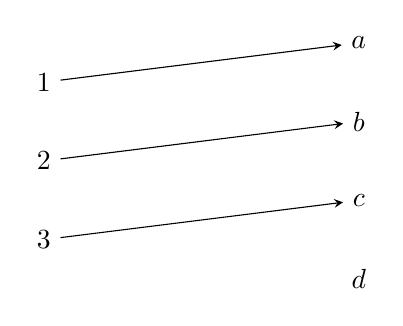
\begin{tikzpicture}[>=stealth, node distance=2cm]
% A nodes (left)
\node (A1) at (0,1) {1};
\node (A2) at (0,0) {2};
\node (A3) at (0,-1) {3};

% B nodes (right)
\node (B1) at (4,1.5) {$a$};
\node (B2) at (4,0.5) {$b$};
\node (B3) at (4,-0.5) {$c$};
\node (B4) at (4,-1.5) {$d$};

% f arrows
\draw[->] (A1) -- (B1);
\draw[->] (A2) -- (B2);
\draw[->] (A3) -- (B3);
\end{tikzpicture}
\end{minipage}
\hspace{0.05\textwidth}
\begin{minipage}{0.45\textwidth}
\centering
\textbf{$g : Y \to X$}

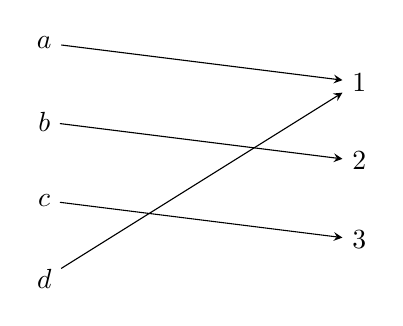
\begin{tikzpicture}[>=stealth, node distance=2cm]
% B nodes (left)
\node (B1) at (0,1.5) {$a$};
\node (B2) at (0,0.5) {$b$};
\node (B3) at (0,-0.5) {$c$};
\node (B4) at (0,-1.5) {$d$};

% A nodes (right)
\node (A1) at (4,1) {1};
\node (A2) at (4,0) {2};
\node (A3) at (4,-1) {3};

% g arrows
\draw[->] (B1) -- (A1);
\draw[->] (B2) -- (A2);
\draw[->] (B3) -- (A3);
\draw[->] (B4) -- (A1); % g(d) = 1 (arbitrary)
\end{tikzpicture}
\end{minipage}
}
\end{center}

Then $\forall x \in X$, $g(f(x)) = x$, so $g$ is a left inverse of $f$.

\subsection{Surjective Case}

If $f : X \to Y$ is surjective, then there exists a right inverse $h : Y \to X$ such that $f(h(y)) = y$, $\forall y \in Y$.

\textbf{Example:}

Let $X = \{1,2,3,4\}$ and $Y = \{a,b\}$.

Define $f : X \to Y$ by

\[
f(1) = a, \quad f(2) = b, \quad f(3) = a, \quad f(4) = b
\]

Then $f$ is surjective but not injective.

A right inverse $h : Y \to X$ may be defined as

\[
h(a) = 1, \quad h(b) = 2
\]

\begin{center}
\fbox{
\begin{minipage}{0.45\textwidth}
\centering
\textbf{$f : X \to Y$}

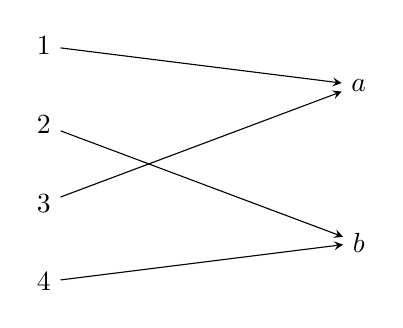
\begin{tikzpicture}[>=stealth, node distance=2cm]

\node (A1) at (0,1.5) {1};
\node (A2) at (0,0.5) {2};
\node (A3) at (0,-0.5) {3};
\node (A4) at (0,-1.5) {4};
\node (B1) at (4,1) {$a$};
\node (B2) at (4,-1) {$b$};
\draw[->] (A1) -- (B1);
\draw[->] (A3) -- (B1);
\draw[->] (A2) -- (B2);
\draw[->] (A4) -- (B2);
\end{tikzpicture}
\end{minipage}
\hspace{0.05\textwidth}
\begin{minipage}{0.45\textwidth}
\centering
\textbf{$h : Y \to X$}

\begin{tikzpicture}[>=stealth, node distance=2cm]

\node (B1) at (0,1) {$a$};
\node (B2) at (0,-1) {$b$};


\node (A1) at (4,1.5) {1};
\node (A2) at (4,0.5) {2};
\node (A3) at (4,-0.5) {3};
\node (A4) at (4,-1.5) {4};


\draw[->] (B1) -- (A1);
\draw[->] (B2) -- (A2);
\end{tikzpicture}
\end{minipage}
}
\end{center}.

Then $\forall y \in Y$, $f(h(y)) = y$, so $h$ is a right inverse of $f$.

\subsection{Bijective Case}

If $f : X \to Y$ is bijective, then there exists a function $f^{-1} : Y \to X$ such that

\[
f^{-1}(f(x)) = x ,\forall x \in X \ \land \ f(f^{-1}(y)) = y, \ \forall y \in Y
\]

\textbf{Example:}

Let $X = \{1,2,3\}$ and $Y = \{a,b,c\}$ with

\[
f(1) = a, \quad f(2) = b, \quad f(3) = c
\]

Then $f$ is bijective. Its inverse $f^{-1}$ satisfies

\[
f^{-1}(a) = 1, \quad f^{-1}(b) = 2, \quad f^{-1}(c) = 3
\]

\begin{center}
\fbox{
\begin{minipage}{0.45\textwidth}
\centering
\textbf{$f : X \to Y$}

\begin{tikzpicture}[>=stealth, node distance=2cm]
% A nodes
\node (A1) at (0,1) {1};
\node (A2) at (0,0) {2};
\node (A3) at (0,-1) {3};

% B nodes
\node (B1) at (4,1) {$a$};
\node (B2) at (4,0) {$b$};
\node (B3) at (4,-1) {$c$};

% Arrows for f
\draw[->] (A1) -- (B1);
\draw[->] (A2) -- (B2);
\draw[->] (A3) -- (B3);
\end{tikzpicture}
\end{minipage}
\hspace{0.05\textwidth}
\begin{minipage}{0.45\textwidth}
\centering
\textbf{$f^{-1} : Y \to X$}

\begin{tikzpicture}[>=stealth, node distance=2cm]
\node (B1) at (0,1) {$a$};
\node (B2) at (0,0) {$b$};
\node (B3) at (0,-1) {$c$};
\node (A1) at (4,1) {1};
\node (A2) at (4,0) {2};
\node (A3) at (4,-1) {3};

\draw[->] (B1) -- (A1);
\draw[->] (B2) -- (A2);
\draw[->] (B3) -- (A3);
\end{tikzpicture}
\end{minipage}
}
\end{center}

\newpage
\subsection{Uniqueness of Inverse}

If $f : X \to Y$ has a left inverse $g$ and a right inverse $h$, then $g = h$. Then, every function has at most one inverse.

Formally:


\[\forall f: X \to Y, \forall g, h: Y \to X \]
\[\left[(g \circ f = \text{id}_X) \land (f \circ g = \text{id}_Y) \land (h \circ f = \text{id}_X) \land (f \circ h = \text{id}_Y)\right] \to g = h\]

\begin{center}
\fbox{
\begin{minipage}{0.45\textwidth}
\centering
\textbf{$f : X \to Y$}

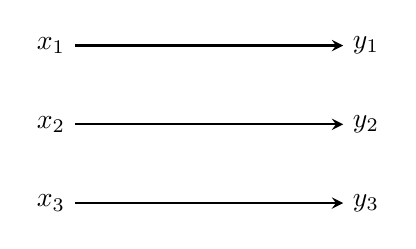
\begin{tikzpicture}[>=stealth]

% X nodes
\node (x1) at (0,1) {$x_1$};
\node (x2) at (0,0) {$x_2$};
\node (x3) at (0,-1) {$x_3$};

% Y nodes
\node (y1) at (4,1) {$y_1$};
\node (y2) at (4,0) {$y_2$};
\node (y3) at (4,-1) {$y_3$};

% Arrows f
\draw[->, thick] (x1) -- (y1);
\draw[->, thick] (x2) -- (y2);
\draw[->, thick] (x3) -- (y3);

\end{tikzpicture}
\end{minipage}
\hspace{0.05\textwidth}
\begin{minipage}{0.45\textwidth}
\centering
\textbf{$g,h : Y \to X$}

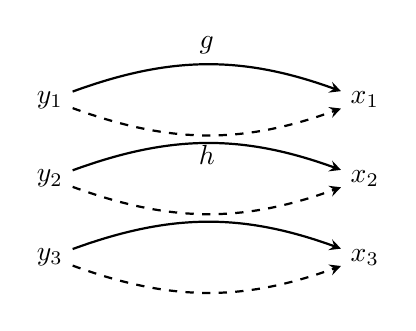
\begin{tikzpicture}[>=stealth]

\node (y1) at (0,1) {$y_1$};
\node (y2) at (0,0) {$y_2$};
\node (y3) at (0,-1) {$y_3$};

\node (x1) at (4,1) {$x_1$};
\node (x2) at (4,0) {$x_2$};
\node (x3) at (4,-1) {$x_3$};

\draw[->, thick, bend left=20] (y1) to node[above] {$g$} (x1);
\draw[->, thick, bend left=20] (y2) to (x2);
\draw[->, thick, bend left=20] (y3) to (x3);

\draw[->, thick, dashed, bend right=20] (y1) to node[below] {$h$} (x1);
\draw[->, thick, dashed, bend right=20] (y2) to (x2);
\draw[->, thick, dashed, bend right=20] (y3) to (x3);

\end{tikzpicture}
\end{minipage}
}
\end{center}


\begin{enumerate}
    \item \textbf{Example 1:}

    Let  

    \[
    X = \{1, 2, 3\}, \quad Y = \{a, b, c\}
    \]

    Define  
    
    \[
    f : X \to Y, \quad f(1) = a, \; f(2) = b, \; f(3) = c
    \]

    Then $f$ is bijective.

    Let  
    
    \[
    g : Y \to X, \quad g(a) = 1, \; g(b) = 2, \; g(c) = 3
    \]

    and  
    
    \[
    h : Y \to X, \quad h(a) = 1, \; h(b) = 2, \; h(c) = 3
    \]

    Then  
    
    \[
    g(f(x)) = x \quad \text{and} \quad f(h(y)) = y
    \]

    Thus $g$ is a left inverse, $h$ is a right inverse, and  
    
    \[
    g = h = f^{-1}
    \]

    Hence, the inverse of $f$ is unique.

    \item \textbf{Example 2:}

    Let  
    
    \[
    f : \mathbb{N} \to \mathbb{Q}, \quad f(n) = n
    \]

    where we regard $\mathbb{N} \subset \mathbb{Q}$. Then $f$ is injective but not surjective, since many rational numbers (e.g. $\frac{1}{2}, \frac{3}{4}$) are not images of any natural number.

    Define  
    
    \[
    g : \mathbb{Q} \to \mathbb{N}, \quad
    g(q) = 
    \displaystyle\begin{cases}
    n, & \text{if } q = n \in \mathbb{N} \\
    1, & \text{otherwise}
    \end{cases}
    \]

    Then $\forall n \in \mathbb{N}$,  
    
    \[
    g(f(n)) = g(n) = n
    \]

    so $g$ is a left inverse of $f$.

    However, $f$ has no right inverse, since it is not surjective, there is no $h : \mathbb{Q} \to \mathbb{N}$ such that  
    
    \[
    f(h(q)) = q, \forall q \in \mathbb{Q}.
    \]

    Hence, $f$ has a left inverse but no right inverse, and therefore no true inverse. If a true inverse existed, it would be unique.
\end{enumerate}

\section{Enumerations and Countable Sets}

\subsection{Enumeration}

Let $A$ be a non-empty set. An \emph{enumeration} of $A$ is an ordered list

\[
(a_1,a_2,a_3,\dots)
\]

of elements of $A$ such that every element of $A$ appears at a finite position in the list.
Equivalently, an enumeration of a non-empty set $A$ is a surjective function

\[
f : \mathbb{Z}^+ \to A, \qquad \mathbb{Z}^+ = \{1,2,3,\dots\},
\]

where

\[
f(n)=a_n \quad \forall n\in\mathbb{Z}^+.
\]

Surjectivity ensures that every element of $A$ appears at least once:

\[
\forall a\in A\;\exists n\in\mathbb{Z}^+ \text{ such that } f(n)=a.
\]


\newpage


\begin{enumerate}

\item \textbf{Example 1:}

Let

\[
A=\{2k \mid k\in\mathbb{Z}^+\}.
\]

Define $f:\mathbb{Z}^+\to A$ by

\[
f(n)=2n.
\]

Then the enumeration is

\[
\begin{array}{c|ccccccccccc}
n        & 1 & 2 & 3 & 4 & 5 & 6 & 7 & 8 & 9 & 10 & \dots \\ \hline
f(n)     & 2 & 4 & 6 & 8 & 10 & 12 & 14 & 16 & 18 & 20 & \dots
\end{array}
\]


\item \textbf{Example 2:}

Define $f:\mathbb{Z}^+\to\mathbb{Z}$ by

\[
f(n)=
\begin{cases}
0, & n=1,\\[1mm]
\dfrac{n}{2}, & n \text{ even},\\[2mm]
-\dfrac{n-1}{2}, & n \text{ odd and } n>1.
\end{cases}
\]

We show that $f$ is bijective.

Surjectivity:

For any $z\in\mathbb{Z}$:

\begin{enumerate}
\item If $z=0$, then $f(1)=0$.
\item If $z=k>0$, then $f(2k)=k$.
\item If $z=-k<0$, then $f(2k+1)=-k$.
\end{enumerate}

Injectivity:

If $f(m)=f(n)$, then $m=n$, since:

\begin{enumerate}
\item even inputs map to positive integers,
\item odd inputs greater than $1$ map to non-positive integers,
\item and within each case the formulas are injective.
\end{enumerate}

Thus,

\[
\mathbb{Z}\sim\mathbb{Z}^+,
\qquad
|\mathbb{Z}|=\aleph_0.
\]

The enumeration is

\[
\begin{array}{c|ccccccccccc}
n        & 1 & 2 & 3 & 4 & 5 & 6 & 7 & 8 & 9 & 10 & \dots \\ \hline
f(n)     & 0 & 1 & -1 & 2 & -2 & 3 & -3 & 4 & -4 & 5 & \dots
\end{array}
\]


\item \textbf{Example 3:}

Let $\mathbb{B}=\{0,1\}$. An enumeration of $\mathbb{B}^*$ is a surjective function

\[
f:\mathbb{N}\to\mathbb{B}^*.
\]

Define
\[
\begin{aligned}
f(0) &= \varepsilon,\\
f(1) &= 0,\\
f(2) &= 1,\\
f(3) &= 00,\\
f(4) &= 01,\\
f(5) &= 10,\\
f(6) &= 11,\\
&\vdots
\end{aligned}
\]

More generally, for each $n\in\mathbb{N}$, let $k$ be the unique integer such that

\[
2^k-1 < n \le 2^{k+1}-1.
\]

Then $f(n)$ is the binary representation of $n-(2^k-1)$ using exactly $k$ bits.

Hence $\mathbb{B}^*$ is countable.

\end{enumerate}

\subsection{Countable Sets}

A set $A$ is called \emph{countable} if it is either empty or admits an enumeration.

Formally,

\[
A \text{ is countable } \leftrightarrow
\bigl(A=\varnothing\bigr)\;\lor\;
\bigl(\exists f:\mathbb{Z}^+\to A \text{ surjective}\bigr).
\]

Equivalently,

\[
\forall a\in A\;\exists n\in\mathbb{Z}^+ \text{ such that } f(n)=a.
\]

\medskip
\textbf{Example}

Let $f:\mathbb{Z}^+\to\{a,b,c\}$ be defined by

\[
f(1)=a,\;
f(2)=b,\;
f(3)=a,\;
f(4)=c,\;
f(5)=b,\;
f(6)=a,\dots
\]

Define $g$ by selecting the first occurrence of each element:

\[
\begin{aligned}
g(1) &= a,\\
g(2) &= b,\\
g(3) &= c.
\end{aligned}
\]

Then

\[
g:\{1,2,3\}\to\{a,b,c\}
\]

is a bijection. Hence every surjection $f:\mathbb{Z}^+\to A$ induces a bijection onto $A$, and therefore $A$ is countable.

\section{Cantor’s Zig-Zag Method}

Recall

\[
\mathbb{N}^2 = \{\langle n, m \rangle : n, m \in \mathbb{N}\}.
\]

Then we can construct Cantor’s zig-zag method as follows.

Let $\mathbb{N}=\{0,1,2,\dots\}$. Define the bijection

\[
f:\mathbb{N}\to\mathbb{N}^2
\]

by

\[
f(k)=(i,j),
\]

where

\[
n=\left\lfloor \frac{\sqrt{8k+1}-1}{2} \right\rfloor,
\qquad
t=\frac{n(n+1)}{2},
\]

and

\[
i=
\begin{cases}
k-t, & \text{if $n$ is even},\\
n-(k-t), & \text{if $n$ is odd},
\end{cases}
\qquad
j=
\begin{cases}
n-i, & \text{if $n$ is even},\\
k-t, & \text{if $n$ is odd}.
\end{cases}
\]

In detail:

\begin{enumerate}
\item $k=0$
\[
n=\left\lfloor \frac{\sqrt{8\cdot0+1}-1}{2} \right\rfloor=0,
\qquad
t=0,
\]
\[
k-t=0,\quad n \text{ even } \to i=0,\ j=0,
\]
\[
f(0)=(0,0).
\]

\item $k=1$
\[
n=\left\lfloor \frac{\sqrt{8\cdot1+1}-1}{2} \right\rfloor=1,
\qquad
t=1,
\]
\[
k-t=0,\quad n \text{ odd } \to i=1,\ j=0,
\]
\[
f(1)=(1,0).
\]

\item $k=2$
\[
n=\left\lfloor \frac{\sqrt{8\cdot2+1}-1}{2} \right\rfloor=1,
\qquad
t=\frac{1\cdot2}{2}=1,
\]
\[
k-t=1,\quad n \text{ odd } \to i=0,\ j=1,
\]
\[
f(2)=(0,1).
\]

\item $k=4$
\[
n=\left\lfloor \frac{\sqrt{8\cdot4+1}-1}{2} \right\rfloor=2,
\qquad
t=\frac{2\cdot3}{2}=3,
\]
\[
k-t=1,\quad n \text{ even } \to i=1,\ j=1,
\]
\[
f(4)=(1,1).
\]

\item $k=5$
\[
n=\left\lfloor \frac{\sqrt{8\cdot5+1}-1}{2} \right\rfloor=2,
\qquad
t=\frac{2\cdot3}{2}=3,
\]
\[
k-t=2,\quad n \text{ even } \to i=0,\ j=2,
\]
\[
f(5)=(0,2).
\]
\end{enumerate}

We can organize these ordered pairs into an array:

\[
\begin{array}{c|cccccc}
 & 0 & 1 & 2 & 3 & \cdots \\
\hline
0 & \langle 0,0 \rangle & \langle 0,1 \rangle & \langle 0,2 \rangle & \langle 0,3 \rangle & \cdots \\
1 & \langle 1,0 \rangle & \langle 1,1 \rangle & \langle 1,2 \rangle & \langle 1,3 \rangle & \cdots \\
2 & \langle 2,0 \rangle & \langle 2,1 \rangle & \langle 2,2 \rangle & \langle 2,3 \rangle & \cdots \\
3 & \langle 3,0 \rangle & \langle 3,1 \rangle & \langle 3,2 \rangle & \langle 3,3 \rangle & \cdots \\
\vdots & \vdots & \vdots & \vdots & \vdots & \ddots
\end{array}
\]

Clearly, every ordered pair in $\mathbb{N}^2$ appears exactly once in the array. In particular, $\langle n,m\rangle$ appears in the $n$th row and $m$th column.

To organize these elements into a one-dimensional list, we use the following pattern:

\[
\begin{array}{c|ccccccc}
 & 0 & 1 & 2 & 3 & 4 & \cdots \\
\hline
0 & 0 & 1 & 3 & 6 & 10 & \cdots \\
1 & 2 & 4 & 7 & 11 & \cdots & \cdots \\
2 & 5 & 8 & 12 & \cdots & \cdots & \cdots \\
3 & 9 & 13 & \cdots & \cdots & \cdots & \cdots \\
4 & 14 & \cdots & \cdots & \cdots & \cdots & \cdots \\
\vdots & \vdots & \vdots & \vdots & \vdots & \vdots & \ddots
\end{array}
\]

This is Cantor’s zig-zag method, which enumerates $\mathbb{N}^2$ as

\[
\langle 0,0\rangle,\langle 0,1\rangle,\langle 1,0\rangle,
\langle 0,2\rangle,\langle 1,1\rangle,\langle 2,0\rangle,
\langle 0,3\rangle,\langle 1,2\rangle,\langle 2,1\rangle,\langle 3,0\rangle,\dots
\]

Moreover, we can use this method to enumerate ordered triples:

\[
\mathbb{N}^3=\{\langle n,m,k\rangle : n,m,k\in\mathbb{N}\}.
\]

Viewing

\[
\mathbb{N}^3=(\mathbb{N}\times\mathbb{N})\times\mathbb{N}
=\{\langle\langle n,m\rangle,k\rangle : n,m,k\in\mathbb{N}\},
\]

we enumerate $\mathbb{N}^3$ by labeling one axis with $\mathbb{N}$ and the other with $\mathbb{N}^2$:

\[
\begin{array}{c|cccccc}
 & 0 & 1 & 2 & 3 & \cdots \\
\hline
\langle 0,0\rangle & \langle 0,0,0\rangle & \langle 0,0,1\rangle & \langle 0,0,2\rangle & \langle 0,0,3\rangle & \cdots \\
\langle 0,1\rangle & \langle 0,1,0\rangle & \langle 0,1,1\rangle & \langle 0,1,2\rangle & \langle 0,1,3\rangle & \cdots \\
\langle 1,0\rangle & \langle 1,0,0\rangle & \langle 1,0,1\rangle & \langle 1,0,2\rangle & \langle 1,0,3\rangle & \cdots \\
\langle 0,2\rangle & \langle 0,2,0\rangle & \langle 0,2,1\rangle & \langle 0,2,2\rangle & \langle 0,2,3\rangle & \cdots \\
\vdots & \vdots & \vdots & \vdots & \vdots & \ddots
\end{array}
\]

Thus, Cantor’s zig-zag method yields an enumeration of $\mathbb{N}^3$, and similarly of $\mathbb{N}^n$ for any $n\in\mathbb{N}$.

\section{Pairing Functions and Codes}

A function

\[
f : A \times B \to \mathbb{N}
\]

is called an \emph{arithmetical pairing function} if it is a bijection.
We say that \(f\) encodes \(A \times B\), and that \(f(x,y)\) is the code
for \(\langle x,y\rangle\).

We define the pairing function \(g : \mathbb{N}^2 \to \mathbb{N}\) by

\[
g(n,m) = \frac{(n+m)(n+m+1)}{2} + n.
\]

This allows us to calculate the exact index of \(\langle n,m\rangle\)
in the enumeration of \(\mathbb{N}^2\).

In fact, we can define \(g\) directly by making two observations about
the diagonal enumeration of \(\mathbb{N}^2\):

\begin{enumerate}
\item Along a fixed diagonal \(n+m=k\), if the entry in the \(n\)-th row
      and \(m\)-th column has value \(v\), then the entry in the
      \((n+1)\)-st row and \((m-1)\)-st column has value \(v+1\).
\item The first row of the enumeration consists of the triangular numbers
      \(0,1,3,6,\dots\).
\end{enumerate}

The \(k\)-th triangular number is
\[
T_k = \sum_{i=0}^{k} i = \frac{k(k+1)}{2}.
\]

Using these observations, we enumerate \(\mathbb{N}^2\) along diagonals
of constant sum.

Define

\[
g(x,y)=T_{x+y}+x=\frac{(x+y)(x+y+1)}{2}+x,
\]

which enumerates pairs by increasing \(x+y\), and within each diagonal counts from top to bottom (increasing \(x\)).


\textbf{Examples:}

\begin{enumerate}
\item \textbf{Encoding \(\langle 1,2\rangle\).}

\begin{enumerate}
\item Diagonal index:

\[
1+2=3.
\]

\item Triangular number of previous entries:

\[
T_3=\frac{3\cdot4}{2}=6.
\]

\item Add the row index:

\[
g(1,2)=T_3+1=6+1=7.
\]
\end{enumerate}

\[
\begin{array}{c|ccccc}
& 0 & 1 & 2 & 3 & \cdots\\ \hline
0 & 0 & 1 & 3 & 6 & \cdots\\
1 & 2 & 4 & \boxed{7} & 11 & \cdots\\
2 & 5 & 8 & 12 & 17 & \cdots\\
3 & 9 & 13 & 18 & 24 & \cdots\\
\vdots & \vdots & \vdots & \vdots & \vdots & \ddots
\end{array}
\]

\item \textbf{Encoding \(\langle 2,3\rangle\).}

\begin{enumerate}
\item Diagonal index:
\[
2+3=5.
\]

\item Triangular number:
\[
T_5=\frac{5\cdot6}{2}=15.
\]

\item Add the row index:
\[
g(2,3)=T_5+2=15+2=17.
\]
\end{enumerate}

\[
\begin{array}{c|ccccc}
g(x,y) & 0 & 1 & 2 & 3 & 4\\ \hline
0 & 0 & 1 & 3 & 6 & 10\\
1 & 2 & 4 & 7 & 11 & 16\\
2 & 5 & 8 & 12 & \boxed{17} & 23\\
3 & 9 & 13 & 18 & 24 & 31\\
4 & 14 & 19 & 25 & 32 & 40
\end{array}
\]


Since we already know the pattern, it is easy to assign the value for every pair directly without recomputing triangular numbers. For example:

\[
g(1,1)=4,\quad g(1,2)=7,\quad g(1,3)=11,\dots
\]

Extending the row-offset pairing to $\mathbb{N}^3$:

\[
G(x,y,z) = g(g(x,y),\,z),
\]

where

\[
g(x,y) = T_{x+y} + x
= \frac{(x+y)(x+y+1)}{2} + x .
\]

Then

\[
G(x,y,z)
= \frac{\left( \frac{(x+y)(x+y+1)}{2} + x + z \right)
\left( \frac{(x+y)(x+y+1)}{2} + x + z + 1 \right)}{2}
+ \frac{(x+y)(x+y+1)}{2} + x .
\]

For compactness, set

\[
A=\frac{(x+y)(x+y+1)}{2}+x .
\]

Then

\[
\boxed{\,G(x,y,z)=\frac{(A+z)(A+z+1)}{2}+A\,}
\qquad\text{with}\qquad
A=\frac{(x+y)(x+y+1)}{2}+x .
\]

\item  \textbf{Encoding \(\langle 1,2,3\rangle\).}

First,

\[
g(1,2) = T_{3} + 1
= \frac{3\cdot4}{2} + 1
= 7 .
\]

Second,

\[
G(1,2,3) = g(7,3)
= T_{10} + 7
= \frac{10\cdot11}{2} + 7
= 62 .
\]

Thus,

\[
\boxed{G(1,2,3)=62.}
\]

\[
\begin{array}{c|cccc}
G(x,y,3) & 0 & 1 & 2 & 3 \\ \hline
0 & 6 & 11 & 24 & 51 \\
1 & 17 & 32 & \boxed{62} & 116 \\
2 & 41 & 74 & 132 & 227 \\
3 & 87 & 149 & 249 & 402
\end{array}
\]

\item  \textbf{Encoding $\langle2, 1, 3\rangle$}:

Firstly,

\[
g(2,1) = T_{2+1} + 2 = T_3 + 2 = \displaystyle\frac{3 \cdot 4}{2} + 2 = 6 + 2 = 8
\]

Secondly,

\[
G(2,1,3) = g(8,3) = T_{8+3} + 8 = T_{11} + 8 = \displaystyle\frac{11 \cdot 12}{2} + 8 = 66 + 8 = 74
\]

Thus,

\[
\boxed{G(2,1,3) = 74.}
\]

\[
\begin{array}{c|cccc}
G(2,1,3) & 0 & 1 & 2 & 3 \\
\hline
0 & 6 & 11 & 24 & 51 \\
1 & 17 & 32 & 62 & 116 \\
2 & 41 & \boxed{74} & 132 & 227 \\
3 & 87 & 149 & 249 & 402 \\
\end{array}
\]

\end{enumerate}

There are other enumerations of \(\mathbb{N}^2\) that make it easier to determine
inverse functions. Rather than visualizing the enumeration in a grid, we begin with the natural
numbers viewed as initially empty positions, which we then fill successively
with ordered pairs \(\langle n,m\rangle\).

We begin with pairs whose first component is \(0\), that is, pairs of the form
\(\langle 0,m\rangle\). Place \(\langle 0,0\rangle\) in the first position, then skip one position and
place \(\langle 0,1\rangle\), skip again and place \(\langle 0,2\rangle\), and so on.

Recall the grid representation of \(\mathbb{N}^2\):

\[
\begin{array}{c|cccccc}
& 0 & 1 & 2 & 3 & \cdots \\ \hline
0 & \langle 0,0\rangle & \langle 0,1\rangle & \langle 0,2\rangle & \langle 0,3\rangle & \cdots \\
1 & \langle 1,0\rangle & \langle 1,1\rangle & \langle 1,2\rangle & \langle 1,3\rangle & \cdots \\
2 & \langle 2,0\rangle & \langle 2,1\rangle & \langle 2,2\rangle & \langle 2,3\rangle & \cdots \\
3 & \langle 3,0\rangle & \langle 3,1\rangle & \langle 3,2\rangle & \langle 3,3\rangle & \cdots \\
\vdots & \vdots & \vdots & \vdots & \vdots & \ddots
\end{array}
\]

Initially, the enumeration appears as follows:

\[
\begin{array}{lcccccccccc}
\textbf{Position:} & 1 & 2 & 3 & 4 & 5 & 6 & 7 & 8 & 9 & \cdots \\
\textbf{Pair:}
& \langle 0,0\rangle
& 
& \langle 0,1\rangle
& 
& \langle 0,2\rangle
& 
& \langle 0,3\rangle
& 
& \langle 0,4\rangle
\end{array}
\]

Since \(2^0=1\), the pairs \(\langle 0,m\rangle\) occupy every odd position.
Next, insert the pairs \(\langle 1,m\rangle\).
Because \(2^1=2\), these occupy every second remaining empty position:

\[
\begin{array}{lcccccccccc}
\textbf{Position:} & 1 & 2 & 3 & 4 & 5 & 6 & 7 & 8 & 9 & 10 \\
\textbf{Pair:}
& \langle 0,0\rangle
& \langle 1,0\rangle
& \langle 0,1\rangle
& 
& \langle 0,2\rangle
& \langle 1,1\rangle
& \langle 0,3\rangle
& 
& \langle 0,4\rangle
\end{array}
\]

Continuing this process for \(\langle 2,m\rangle\), \(\langle 3,m\rangle\), and so
on yields the enumeration:

\[
\begin{array}{lcccccccccc}
\textbf{Position:} & 1 & 2 & 3 & 4 & 5 & 6 & 7 & 8 & 9 & 10 \\
\textbf{Pair:}
& \langle 0,0\rangle
& \langle 1,0\rangle
& \langle 0,1\rangle
& \langle 2,0\rangle
& \langle 0,2\rangle
& \langle 1,1\rangle
& \langle 0,3\rangle
& \langle 3,0\rangle
& \langle 0,4\rangle
& \langle 1,2\rangle
\end{array}
\]

Numbering positions according to this scheme gives the following table:

\[
\begin{array}{c|ccccccc}
 & 0 & 1 & 2 & 3 & 4 & 5 & \cdots \\ \hline
0 & 1 & 3 & 5 & 7 & 9 & 11 & \cdots \\
1 & 2 & 6 & 10 & 14 & 18 & \cdots & \cdots \\
2 & 4 & 12 & 20 & 28 & \cdots & \cdots & \cdots \\
3 & 8 & 24 & 40 & \cdots & \cdots & \cdots & \cdots \\
4 & 16 & 48 & \cdots & \cdots & \cdots & \cdots & \cdots \\
\vdots & \vdots & \vdots & \vdots & \vdots & \vdots & \vdots & \ddots
\end{array}
\]

For all \(n,m\in\mathbb{N}\), the position of \(\langle n,m\rangle\) in this
enumeration is
\[
\langle n,m\rangle \mapsto 2^n(2m+1).
\]

To shift the enumeration so that it begins at \(0\), define the pairing function
\(h:\mathbb{N}^2\to\mathbb{N}\) by
\[
\boxed{h(n,m)=2^n(2m+1)-1.}
\]

\[
\begin{array}{c|cccccc}
(n,m) & 0 & 1 & 2 & 3 & 4 & 5 \\ \hline
0 & 0 & 2 & 4 & 6 & 8 & 10 \\
1 & 1 & 5 & 9 & 13 & 17 & 21 \\
2 & 3 & 11 & 19 & 27 & 35 & 43 \\
3 & 7 & 23 & 39 & 55 & 71 & 87 \\
4 & 15 & 47 & 79 & 111 & 143 & 175 \\
\vdots & \vdots & \vdots & \vdots & \vdots & \vdots & \ddots
\end{array}
\]

\section{Uncountable Sets}

It is known that, some sets, such as the set $ \mathbb{Z}^+ $ of positive integers, are infinite. So far, we have encountered infinite sets that are all countable. 
For example, the set of even positive integers $E = \{2, 4, 6, 8, \ldots\} $ is countable. Although $E$ seems smaller than $ \mathbb{Z}^+ $, we can pair each element of $E$ with exactly one element of $ \mathbb{Z}^+ $ using the function:

\[
f(n = 2n), \quad \text{for } n \in \mathbb{Z}^+
\]

Specifically

\[\begin{array}{c|cccccccc}
\mathbb{Z}^+ & 1 & 2 & 3 & 4 & 5 & \cdots & n \\
\hline
E & 2 & 4 & 6 & 8 & 10 & \cdots & 2n
\end{array}\]

This function is a bijection from $\mathbb{Z}^+$ to $E$, proving that $E$ is countable. In other words:

\[|E| = |\mathbb{Z}^+|\]

However, there exist infinite sets which do not have this property. 
Such sets are called uncountable. By definition, a set $S$ is countable if there exists a surjective function $ f: \mathbb{Z}^+ \to S $. 
Otherwise, $S$ is uncountable. If a set is uncountable, then no function mapping $\mathbb{Z}^+$ to $S $ can cover all elements of $S$.
Thus, there are more elements in $S$ than there are in $\mathbb{Z}^+$, $$|\mathbb{Z}^+| < |S|$$ To prove a set is uncountable, we must show that no such surjective function can exist. 
Equivalently, the elements of $S$ cannot be enumerated in a one-way infinite list. A powerful technique for demonstrating this is called *Cantor’s diagonal method*.

\begin{enumerate}
    \item \textbf{Example 1}
    
    Suppose, for contradiction, that $\mathbb{B}^\omega$ is countable. Then we could list all its elements:
    
    \[s_1, s_2, s_3, s_4, \ldots s_n \]
    
    This means there exists a surjective function $f: \mathbb{Z}^+ \to \mathbb{B}^\omega$ with $f(i) = s_i$, so:
    
    \[\mathbb{B}^\omega = \{s_1, s_2, s_3, \ldots\}\]
    
    Each $s_i$ is itself an infinite binary sequence, written as:
    
    \[s_i = \left( s_i(1),\ s_i(2),\ s_i(3),\ \ldots \right)\]
    
    where \[s_i(j) \in \{0,1\}, \forall j \in \mathbb{Z}^+\]
    
    We may organize this list into an infinite array where each row corresponds to a sequence and each column to a digit in the sequence:
    
    \[\begin{array}{c|cccccc}
    & 1 & 2 & 3 & 4 & 5 & \cdots \\
    \hline
    s_1 & \boxed{0} & 1 & 0 & 1 & 1 & \cdots \\
    s_2 & 1 & \boxed{1} & 0 & 0 & 1 & \cdots \\
    s_3 & 0 & 1 & \boxed{0} & 1 & 0 & \cdots \\
    s_4 & 1 & 0 & 1 & \boxed{1} & 0 & \cdots \\
    s_5 & 0 & 1 & 0 & 1 & \boxed{0} & \cdots \\
    \vdots & \vdots & \vdots & \vdots & \vdots & \vdots & \ddots
    \end{array}\]
    
    Define the new sequence:
    
    \[
    \overline{s}(n) =
    \begin{cases}
    1, & \text{if } s_n(n) = 0 \\
    0, & \text{if } s_n(n) = 1
    \end{cases}
    \]
    
    Or equivalently,
    
    \[\forall n\in\mathbb{Z}^+,\quad \overline{s}(n) \ne s_n(n)\]
    
    Flipping the diagonal:
    
    \[\begin{aligned}
    s_1(1) = \boxed{0} &\to \overline{s}(1) = 1 \\
    s_2(2) = \boxed{1} &\to \overline{s}(2) = 0 \\
    s_3(3) = \boxed{0} &\to \overline{s}(3) = 1 \\
    s_4(4) = \boxed{1} &\to \overline{s}(4) = 0 \\
    s_5(5) = \boxed{0} &\to \overline{s}(5) = 1 \\
    \vdots
    \end{aligned}\]
    
    Therefore, \[\overline{s} = (1, 0, 1, 0, 1, \ldots)\]
    
    Then:
    
    \[\forall n\in\mathbb{Z}^+,\ \overline{s}(n)\ne s_n(n)\]
    
    Assume $\exists k\in\mathbb{Z}^+$ such that $\overline{s}=s_k$
    
    \[\overline{s}(k)=s_k(k)\]
    
    But by construction:
    
    \[
    \overline{s}(k) \ne s_k(k)
    \]
    
    This contradiction shows that $\overline{s} \notin \{s_1, s_2, \ldots\}$, even though $\overline{s} \in \mathbb{B}^\omega$. Therefore,
    
    \[\boxed {\mathbb{B}^\omega \ \text{is uncountable}}\]

    \item \textbf{Example 2}
    
    Suppose, for contradiction, that $\mathcal{P}(\mathbb{Z}^+)$ is countable. Then there exists a bijection:
    
    \[
    f : \mathbb{Z}^+ \to \mathcal{P}(\mathbb{Z}^+)
    \]
    
    Enumerate all subsets of $\mathbb{Z}^+$ as:
    
    \[
    \mathcal{P}(\mathbb{Z}^+) = \{ Z_1, Z_2, Z_3, \dots \}
    \]
    
    where $ f(n) = Z_n $.
    
    Define the diagonal set:
    
    \[
    \overline{Z} = \{ n \in \mathbb{Z}^+ \mid n \notin Z_n \}
    \]
    
    Equivalently, for each $n \in \mathbb{Z}^+$:
    
    \[
    n \in \overline{Z} \leftrightarrow n \notin Z_n
    \]
    
    Consider this enumeration:
    
    \[
    \begin{array}{c|ccccc}
     & 1 & 2 & 3 & 4 & 5 \\\hline
    Z_1 & \boxed{1} & 2 & 3 & 4 & 5 \\
    Z_2 & - & \boxed{2} & - & 4 & - \\
    Z_3 & 1 & 2 & \boxed{-} & - & 5 \\
    Z_4 & - & - & 3 & \boxed{4} & 5 \\
    Z_5 & - & 2 & 3 & - & \boxed{-} \\
    \end{array}
    \]
    
    Diagonal entries correspond to the membership condition $ n \in Z_n $.
    
    Constructing $\overline{Z}$ by flipping diagonal membership:
    
    \[
    \overline{Z} = \{ n \in \mathbb{Z}^+ : n \notin Z_n \}
    \]
    
    From the diagram:
    
    \[
    \overline{Z} = \{3, 5\}
    \]
    
    By construction:
    
    \[
    \forall k \in \mathbb{Z}^+, \quad
    k \in \overline{Z} \leftrightarrow k \notin Z_k
    \quad \to \quad
    \overline{Z} \ne Z_k
    \]
    
    but by definition:
    
    \[
    (k \in \overline{Z}) \leftrightarrow (k \notin Z_k)
    \]
    
    Therefore:
    
    \[
    \forall k \in \mathbb{Z}^+, \; \overline{Z} \ne Z_k
    \]
    
    In detail:
    
    \begin{enumerate}
    \item \textbf{$\overline{Z} \ne Z_1$} since $1 \notin \overline{Z}$ but $1 \in Z_1$,
    \item \textbf{$\overline{Z} \ne Z_2$} since $2 \notin \overline{Z}$ but $2 \in Z_2$,
    \item \textbf{$\overline{Z} \ne Z_3$} since $3 \in \overline{Z}$ but $3 \notin Z_3$.
    \end{enumerate}
    
    Thus:
    
    \[
    \forall k \in \mathbb{Z}^+, \; \overline{Z} \ne Z_k
    \]
    
    and hence $\overline{Z}$ is not in the enumeration $\{Z_1, Z_2, Z_3, \dots\}$. Contradiction.
    
    Therefore:
    \[
    |\mathcal{P}(\mathbb{Z}^+)| > |\mathbb{Z}^+|
    \]
    
    \[
    \boxed{\mathcal{P}(\mathbb{Z}^+) \text{ is uncountable.}}
    \]

    
\end{enumerate}


Recall that for two sets $A$ and $B$, the Cartesian product is defined as

\[
A \times B = \{ (a,b) \mid a \in A \land b \in B \}.
\]

For three sets $A$, $B$, and $C$:

\[
A \times B \times C = \{ (a,b,c) \mid a \in A \land b \in B \land c \in C \}.
\]

In fact, we can extend this idea to a finite collection of sets, and then to an infinite one. Suppose we have a finite index set

\[
I = \{1, 2, \dots, n\},
\]

and a collection of sets

\[
\{A_i\}_{i \in I}.
\]

Then the Cartesian product is defined as

\[
\displaystyle\prod_{i=1}^{n} A_i = \{ (a_1, a_2, \dots, a_n) \mid a_i \in A_i \text{ for each } i = 1, 2, \dots, n \}.
\]

This is the set of all $n$-tuples, where the $i^{\text{th}}$ coordinate comes from $A_i$.

Now, let $I$ be any index set, possibly infinite. We have a family of sets $\{A_i\}_{i \in I}$. We can no longer write down a tuple like $(a_1, a_2, \dots)$, since there are infinitely many coordinates. Instead, we define elements as functions.

\[
\displaystyle\prod_{i \in I} A_i
    =
    \left\{
        f : I \to \bigcup_{i \in I} A_i
        \,\middle|\,
        \forall i \in I,\; f(i) \in A_i
    \right\}.
\]

Each $f$ acts like an infinite tuple:

\[
f = (f(i))_{i \in I}.
\]

Thus, we can think informally of an element of the product as

\[
(a_i)_{i \in I} \quad \text{where } a_i \in A_i.
\]

\paragraph{Example:}
Let 
\[A_i = \{0,1\}\] 
for each 
\[i \in \mathbb{N}.\]

Then the infinite Cartesian product is

\[
\displaystyle\prod_{i \in \mathbb{N}} A_i = \{ f : \mathbb{N} \to \{0,1\} \}.
\]

Each element $f$ of this product is a function that assigns to every natural number $i$ either $0$ or $1$. Equivalently, each $f$ corresponds to an infinite binary sequence:

\[
f = (f(1), f(2), f(3), \ldots) = (0,1,1,0,0,1,\ldots).
\]

Thus, the product can be written more compactly as

\[
\{0,1\}^{\mathbb{N}} = \text{the set of all infinite binary sequences.}
\]

Suppose, for the sake of contradiction, that we could list all such sequences:

\[
f_1, f_2, f_3, \ldots
\]

where each 
\[f_k : \mathbb{N} \to \{0,1\}.\]

Then, define a new sequence
\[\overline{f} : \mathbb{N} \to \{0,1\}\]
by flipping the diagonal entries:

\[
\overline{f}(n) =
\begin{cases}
1, & \text{if } f_n(n) = 0, \\
0, & \text{if } f_n(n) = 1.
\end{cases}
\]

Or equivalently,

\[
\forall n \in \mathbb{N}, \quad \overline{f}(n) \ne f_n(n).
\]

By construction, $\overline{f}$ differs from each $f_n$ at least in the $n$-th position. Therefore, $\overline{f}$ cannot appear anywhere in the list $(f_1, f_2, f_3, \ldots)$.

This contradiction shows that no such enumeration exists, in other words,

\[
\{0,1\}^{\mathbb{N}} \text{ is uncountable} \ \text{or equivalently,} \
\left| \{0,1\}^{\mathbb{N}} \right| = 2^{\aleph_0}.
\]

Specifically:

\begin{enumerate}
    \item Constant zero function: $f(n) = 0 \quad \forall n \in \mathbb{N}$. Sequence: $(0,0,0,0,\ldots)$
    \item Constant one function: $f(n) = 1 \quad \forall n \in \mathbb{N}$. Sequence: $(1,1,1,1,\ldots)$
    \item Alternating sequence: $f(n) = \begin{cases} 0, & \text{if } n \text{ is odd},\\ 1, & \text{if } n \text{ is even.} \end{cases}$ Sequence: $(0,1,0,1,0,1,\ldots)$
    \item Prime indicator function: $f(n) = \begin{cases} 1, & \text{if } n \text{ is prime},\\ 0, & \text{otherwise.} \end{cases}$ Sequence: $(0,1,1,0,1,0,1,0,0,0,1,\ldots)$
    \item The diagonal function from Cantor’s argument: $\overline{f}(n) \ne f_n(n)$.
\end{enumerate}

This set $\{0,1\}^{\mathbb{N}}$ has the same cardinality as the real numbers $\mathbb{R}$, known as the cardinality of the continuum.

Hence,

\[
\boxed{\displaystyle\prod_{i \in \mathbb{N}} \{0,1\} \text{ is uncountable.}}
\]

\section{Reduction and Equinumerosity}

\subsection{Reduction}

A \textit{reduction} from a set $A$ to a set $B$ is a surjective function
\[
f : A \to B.
\]
If such a surjection exists, we say that the cardinality of $A$ is greater than or equal to the cardinality of $B$, and thus
\[
|A| \ge |B|.
\]
Equivalently, the existence of a surjective function $f : A \to B$ implies the existence of an injective function $g : B \to A$, that is,
\[
\exists f : A \to B \; (\text{surjective}) \;\; \leftrightarrow \;\;
\exists g : B \to A \; (\text{injective}).
\]

\begin{enumerate}
    \item \textbf{Example 1} \\
    Let $\mathbb{N} $ and $2\mathbb{N} = \{0, 2, 4, 6, \ldots\} $. Define $ f : \mathbb{N} \to 2\mathbb{N} $ by  
    \[ f(n) = 2n. \]
    Then $ f $ is surjective, since for every even number $ 2k \in 2\mathbb{N} $, there exists $ n = k \in \mathbb{N} $ such that $ f(n) = 2k $. Thus, there exists an injection $ g : 2\mathbb{N} \to \mathbb{N} $, for instance  
    \[ g(2k) = k. \]
    Hence, \[ |\mathbb{N}| \ge |2\mathbb{N}|. \]

    \item \textbf{Example 2} \\
    Reduction from $\mathcal{P}(\mathbb{Z}^+)$ to $\mathbb{B}^\omega$. Suppose $\mathcal{P}(\mathbb{Z}^+)$ is countable with enumeration:
    \[ Z_1, Z_2, Z_3, \dots \]
    Define $f : \mathcal{P}(\mathbb{Z}^+) \to \mathbb{B}^\omega$ by:
    \[
    f(Z) = (b_1, b_2, b_3, \ldots)
    \quad \text{where} \quad
    b_n =
    \begin{cases}
    1 & \text{if } n \in Z \\
    0 & \text{if } n \notin Z
    \end{cases}
    \]
    According to the definition of $f$, each subset $ Z \subseteq \mathbb{Z}^+$ is represented by its characteristic sequence in $ \mathbb{B}^\omega$. a sequence of 1’s and 0’s indicating which natural numbers belong to $ Z$. For example:
    \[
    \begin{aligned}
    f(\{1,3,5,7,\ldots\}) &= (1,0,1,0,1,0,1,\ldots),\\
    f(\{2,4,6,8,\ldots\}) &= (0,1,0,1,0,1,0,\ldots),\\
    f(\varnothing) &= (0,0,0,0,\ldots),\\
    f(\mathbb{Z}^+) &= (1,1,1,1,\ldots).
    \end{aligned}
    \]
    We now verify that the function $f$ defined above is surjectivy, that is, for every sequence $s \in \mathbb{B}^\omega$, there exists some subset $Z \subseteq \mathbb{Z}^+$ such that $f(Z) = s$.
    
    For any $s = (b_1, b_2, b_3, \ldots) \in \mathbb{B}^\omega$, define
    \[ Z = \{ n \in \mathbb{Z}^+ : s(n) = 1 \}. \]
    By construction, this subset $Z$ produces exactly the sequence $s$ when substituted into the definition of $f$; that is,
    \[ f(Z) = s. \]
    Hence, $f$ is surjective:
    \[ f : \mathcal{P}(\mathbb{Z}^+) \to \mathbb{B}^\omega. \]
    Therefore, the enumeration $f(Z_1), f(Z_2), f(Z_3), \ldots$ would list all elements of $\mathbb{B}^\omega$, implying that $\mathbb{B}^\omega$ is countable.  However, $\mathbb{B}^\omega$ is uncountable (by Cantor’s diagonal argument). This contradiction shows that $\mathcal{P}(\mathbb{Z}^+)$ must be uncountable. We conclude that, 
    \[ |\mathcal{P}(\mathbb{Z}^+)| \ge |\mathbb{B}^\omega|. \]
    However, the function $g : \mathbb{B}^\omega \to \{0,1\}$ defined by $g(s) = s(1)$ is also surjective, yet it does not imply that $\{0,1\}$ is uncountable, since
    \[ |\mathbb{B}^\omega| \ge |\{0,1\}| = 2 \]
    is trivially true. Thus, the direction of the surjection determines the direction of the inequality in cardinality. To illustrate the importance of surjectivity, define $h : \mathbb{Z}^+ \to \mathbb{B}^\omega$ by
    \[ h(n) = (\underbrace{0,0,\ldots,0}_{n}, 1, 0, 0, \ldots). \]
    Here, $(1,1,1,1,\ldots) \notin \operatorname{Im}(h)$, so $h$ is not surjective. Consequently, $h$ cannot be used to infer any relationship between $|\mathbb{Z}^+|$ and $|\mathbb{B}^\omega|$.
\end{enumerate}

\subsection{2Equinumerosity}

A set $A$ is \textit{equinumerous} with a set $B$, written $A \approx B$, if and only if there exists a bijection
\[
f : A \to B.
\]
That is,
\[
A \approx B \;\leftrightarrow \; \exists f : A \to B \; (\text{bijective}).
\]
The relation $\approx$ is an equivalence relation on the class of all sets, since it satisfies the following properties:

\begin{enumerate}
    \item Reflexive
    \[ \text{Id}_A : A \to A, \quad \text{where } \forall x \in A, \; \text{Id}_A(x) = x. \]
    \[ \text{Id}_A \text{ is a bijection } \to A \approx A. \]
    

    \item Symmetric \\
    Suppose $A \approx B$, i.e., there is a bijection $f : A \to B$. Since $f$ is bijective, its inverse $f^{-1}$ exists and is also bijective. Hence, $f^{-1} : B \to A$ is a bijection, so $B \approx A$.
    

    \item Transitive
    \[ A \approx B \;\wedge\; B \approx C \;\to\; \exists f : A \to B, \; \exists g : B \to C \text{ such that } f, g \text{ are bijective.} \]
    \[ (g \circ f) : A \to C \text{ is bijective. Therefore } A \approx C. \]
    
\end{enumerate}


\begin{enumerate}
    \item \textbf{Example 1:} \\
    It is well known that, \[|\mathbb{N}| = |\mathbb{Z}| = |\mathbb{Q}| = \aleph_0\]
    In detail: 
    \begin{enumerate}
        \item $\mathbb{N}$ and $\mathbb{Z}$ 
        \[f(n) = \begin{cases}
        \displaystyle\frac{n}{2} & \text{if } n \text{ is even} \\
        -\displaystyle\frac{n-1}{2} & \text{if } n \text{ is odd}
        \end{cases}\]
        \[\begin{array}{c|cccccccccc}
        \mathbb{N} & 0 & 1 & 2 & 3 & 4 & 5 & 6 & 7 & \cdots \\
        \hline
        \mathbb{Z} & 0 & -1 & 1 & -2 & 2 & -3 & 3 & -4 & \cdots
        \end{array}\]

        \item $\mathbb{N}$ and $\mathbb{Q}^+$ \\
        Using Cantor's diagonal enumeration (pairing method):
        \[\begin{array}{c|cccccccccc}
        \mathbb{N} & 1 & 2 & 3 & 4 & 5 & 6 & 7 & 8 & \cdots \\
        \hline
        \mathbb{Q}^+ & \displaystyle\frac{1}{1} & \displaystyle\frac{2}{1} & \displaystyle\frac{1}{2} & \displaystyle\frac{1}{3} & \displaystyle\frac{3}{1} & \displaystyle\frac{4}{1} & \displaystyle\frac{3}{2} & \displaystyle\frac{2}{3} & \cdots
        \end{array}\]
        Following the diagonal path through the grid of fractions $\displaystyle\frac{p}{q}$, skipping duplicates.
        
    \end{enumerate}

    \item \textbf{Example 2: } \\
    Nonetheless, there is no direct bijection function from $\mathbb{N}$ into $[0,1]$ $\in \mathbb{R}$, as proven by Cantor's Diagonal Argument. Specifically, suppose we have a function $f: \mathbb{N} \to [0,1] $ that attempts to enumerate all real numbers in the interval [0, 1].
    \[\begin{array}{c|l}
    \mathbb{N} & \ \ \ \ \ \ \ [0,1] \\
    \hline
    0 & 0.1372894651 \\
    1 & 0.4029135702 \\
    2 & 0.7182390045 \\
    3 & 0.5927813409 \\
    \vdots & \ \ \ \ \ \ \ \ \ \ \vdots
    \end{array}\]
    Now, we can construct a new real number $\overline {r} \in [0, 1]$ by altering the $n$-th digit of the $n$-th number in the list.
    \[\begin{array}{c|c|c}
    \mathbb{N} & [0,1] & r \\
    \hline
    0 & 0.\boxed{1}372894651 & 2 \\
    1 & 0.4\boxed{0}29135702 & 1 \\
    2 & 0.71\boxed{8}2390045 & 9 \\
    3 & 0.592\boxed{7}813409 & 8 \\
    \vdots & \vdots & \vdots
    \end{array}\]
    Thus, we have constructed a new number $\overline{r} = 0.2198\ldots$ that differs from every number in the list at least at one decimal place, proving that no function $f: \mathbb{N} \to [0,1]$ can be surjective.
    
    With this in mind, we conclude that $\mathbb{N}$ cannot enumerate $[0, 1] \subseteq \mathbb{R}$. Therefore:
    \[|\mathbb{N}| = \aleph_0 < |[0, 1]| = |\mathbb{R}| = 2^{\aleph_0}\]
    This result is related to the \textit{Continuum Hypothesis $(CH)$}, which states that there is no set whose cardinality is strictly between $\aleph_0$ and $2^{\aleph_0}:$
    \[\nexists S : \aleph_0 < |S| < 2^{\aleph_0}\]
\end{enumerate}

\section{Sets of Different Sizes}

Let $A,B$ be sets. We define the following relations:

\begin{enumerate}
  \item No larger than
  \[
  A \preceq B
  \leftrightarrow  
  \exists f : A \to B \text{ such that } f \text{ is injective.}
  \]

  \item Smaller than
  \[
  A \prec B
  \leftrightarrow  
  \exists f : A \to B \text{ injective, and } \nexists g : A \to B \text{ bijective.}
  \]

  Equivalently,
  \[
  A \prec B
  \leftrightarrow  
  A \preceq B \text{ and } A \not\approx B.
  \]

\end{enumerate}

\section{Cantor’s Theorem}


For any set $A$,
\[
\forall A,\; \neg \exists f : A \to \mathcal{P}(A) \; (\text{surjective}),
\]
which implies
\[
|A| < |\mathcal{P}(A)|.
\]

\emph{Proof}

Suppose, for the sake of contradiction, that there exists a surjection

\[
f : A \to \mathcal{P}(A),
\]

that is, every subset of $A$ is the image of some element of $A$.

Define the set

\[
B = \{\, x \in A \mid x \notin f(x) \,\}.
\]

Thus, $B$ consists of all elements of $A$ that do not belong to their image under $f$.

Since $f$ is assumed to be surjective, there exists some element $x \in A$ such that

\[
f(x) = B.
\]

We now consider two cases:

\begin{enumerate}
  \item Case $x \in B$ 
  By the definition of $B$, this implies $x \notin f(x)$.  
  Since $f(x) = B$, we conclude $x \notin B$, a contradiction.

  \item Case $x \notin B$  
  By the definition of $B$, this implies $x \in f(x) = B$, again a contradiction.
\end{enumerate}

In both cases, we reach a contradiction. Therefore, the assumption that $f$ is surjective must be false. Hence, no surjection exists from $A$ onto $\mathcal{P}(A)$.

Consequently, the power set of any set is strictly larger than the set itself:

\[
|A| < |\mathcal{P}(A)|.
\]

\begin{enumerate}

\item \textbf{Example 1 :}

Let

\[
A = \{1,2\}.
\]

Then

\[
\mathcal{P}(A) = \{\varnothing, \{1\}, \{2\}, \{1,2\}\}.
\]

Any function $f : A \to \mathcal{P}(A)$ can map at most $2$ elements, whereas $\mathcal{P}(A)$ has $4$ elements. Hence, $f$ cannot be surjective.

Thus,

\[
|A| = 2,
\qquad
|\mathcal{P}(A)| = 4,
\]

and clearly,

\[
|A| < |\mathcal{P}(A)|.
\]

\item \textbf{Example 2:}

For the set of natural numbers,

\[
|\mathbb{N}| = \aleph_0,
\qquad
|\mathcal{P}(\mathbb{N})| = 2^{\aleph_0} > \aleph_0.
\]

This shows that the set of all subsets of $\mathbb{N}$ is uncountably infinite.

\end{enumerate}

\section{Cantor–Schröder–Bernstein}

Let $A, B$ be sets. If $A \preceq B$ and $B \preceq A$, then $A \approx B$. Equivalently:
if there exist injective functions 
\[
f: A \to B, \qquad g: B \to A,
\] 
then there exists a bijection 
\[
h: A \to B.
\] 

\emph{proof.}

Define the starting layers in $A$:
\[
A_0 = A \setminus g(B), \qquad
A_{n+1} = g(f(A_n)), \quad n \ge 0.
\]

For $a_0 \in A$, consider the alternating chain:

\[
\begin{array}{ccccccccc}
{A_0} & \xrightarrow{\,f\,} & B & \xrightarrow{\,g\,} & A & \xrightarrow{\,f\,} & B & \xrightarrow{\,g\,} & \dots \\
a_0 \in A_0 & & f(a_0) & & g(f(a_0)) & & f(g(f(a_0))) & & \dots
\end{array}
\]

Similarly, define the starting layers in $B$:

\[
B_0 = B \setminus f(A), \qquad
B_{n+1} = f(g(B_n)), \quad n \ge 0.
\]

\[
\begin{array}{ccccccccc}
\dots & \xleftarrow{\,f\,} & A & \xleftarrow{\,g\,} & B & \xleftarrow{\,f\,} & A & \xleftarrow{\,g\,} & {B_0} \\
\dots & & g(f(g(b_0))) & & f(g(b_0)) & & g(b_0) & & b_0 \in B_0
\end{array}
\]

If, after finitely many steps, this chain leaves $g(B)$, then $a_0 \in X$. Formally,
\[
X = \{\, a \in A \mid \exists n \ge 0 : (g \circ f)^n(a) \notin g(B) \,\},
\]
and equivalently,
\[
X = \bigcup_{n=0}^{\infty} A_n.
\]

Define
\[
Y = A \setminus X = \{\, a \in A \mid \forall n \ge 0 : (g \circ f)^n(a) \in g(B) \,\},
\]
the set of elements that always remain within the image $g(B)$ under repeated application of $f$ and $g$, or equivalently,
\[
Y = \bigcap_{n=0}^{\infty} (A \setminus A_n).
\]

Similarly, define $Z = f(X)$ and $W = B \setminus Z$. We define our bijection $h: A \to B$ as:
\[
h(a) =
\begin{cases}
f(a), & a \in X, \\[2mm]
g^{-1}(a), & a \in Y.
\end{cases}
\]

\begin{enumerate}
\item Injective 

\begin{enumerate}
    \item If $a_1, a_2 \in X$, then $h(a_1)=h(a_2) \to f(a_1)=f(a_2) \to a_1=a_2$.
    \item If $a_1, a_2 \in Y$, then $h(a_1)=h(a_2) \to g^{-1}(a_1)=g^{-1}(a_2) \to a_1=a_2$.
    \item If $a_1 \in X, a_2 \in Y$, then $h(a_1)=h(a_2)$ implies $f(a_1) = g^{-1}(a_2)$, which means $a_2 = g(f(a_1))$. But $a_2 \in Y$ (complement of $X$), while $g(f(a_1)) \in X$. This contradiction ($a_2 \in X \cap Y$) shows $h$ is injective.
\end{enumerate}

\item Surjective
$\forall b \in B$:

\begin{enumerate}
    \item If $b \in f(X)$, then $\exists a \in X$ such that $b = f(a) = h(a)$.
    \item If $b \notin f(X)$, then $g(b) = a$ must be in $Y$ (if $a$ were in $X$, $b$ would be in $f(X)$). Then $h(a) = g^{-1}(g(b)) = b$.
\end{enumerate}

\end{enumerate}
Therefore $h$ is bijective, and $|A| = |B|$.


\textbf{Example:}

Firstly, define injective functions:

\[
f: \mathbb{N} \to \mathbb{N}, \quad f(x) = x,
\]
\[
g: \mathbb{N} \to \mathbb{N}, \quad g(0) = 1, \quad g(y) = y+1 \text{ for } y \ge 1.
\]

The forward roots are:

\[
X_0 = \mathbb{N} \setminus g(\mathbb{N}) = \{0\} \text{ is false here; actually } \mathbb{N} \setminus \{1, 2, \dots\} = \{0\}.
\]

\textit{(Note: In this specific example, $g(\mathbb{N}) = \{1, 2, 3, \dots\}$, so $0 \in A_0$.)}

Continuing the chain:

\[
0 \xrightarrow{\,f\,} 0 \xrightarrow{\,g\,} 1 \xrightarrow{\,f\,} 1 \xrightarrow{\,g\,} 2 \xrightarrow{\,f\,} 2 \cdots
\]

This implies $X = \{0, 1, 2, \dots\} = \mathbb{N}$, and $Y = \varnothing$.

Then the bijection $h: \mathbb{N} \to \mathbb{N}$ is:

\[
h(x) = f(x) = x.
\]

Alternatively, if we define the chain such that $Y_0 = \mathbb{N} \setminus f(\mathbb{N}) = \varnothing$, we follow the construction provided:

\[
h: 1 \mapsto 0, \; 2 \mapsto 1, \; 3 \mapsto 2, \; 4 \mapsto 3, \dots
\]

which is the mapping $h(x) = x-1$.

\end{document}